%***************************************************************************
% Chapter: Karnaugh maps
%***************************************************************************
\chapter{Karnaugh maps}\label{ch06}

\section{Introduction}

% Pull Quote - Marginal Note - Sidebar
\marginpar{Maurice Karnaugh developed this process at Bell Labs in 1953 while designing switching circuits for landline telephones.}

A Karnaugh map, like Boolean algebra, is a tool used to simplify a digital circuit. Keep in mind that ``simplify'' means reducing the number of gates and inputs for each gate and as components are eliminated, not only does the manufacturing cost go down, but the circuit becomes simpler, more stable, and more energy efficient. 

In general, using Boolean Algebra is the easiest way to simplify a circuit involving one to three input variables. For four input variables, Boolean algebra becomes tedious and Karnaugh maps are both faster and easier (and are less prone to error). However, Karnaugh maps become rather complex with five input variables and are generally too difficult to use above six variables (with more than four input variables, a Karnaugh map uses multiple dimensions that become very challenging to manipulate). For five or more input variables, circuit simplification should be done by Quine-McClusky methods  (page \pageref{ASM:sec:quine-mccluskey_simplification_method}) or the use of \ac{CAT} (page \pageref{ASM:sec:automated_tools}).

In theory, any of the methods will work for any number of variables; however, as a practical matter, the guidelines presented in Table \ref{KM:tab:circuit_simplification_methods} work well. Normally, there is no need to resort to \ac{CAT} to simplify a simple equation involving two or three variables since it is much quickly to use either Boolean Algebra or Karnaugh maps. However, for more complex input/output combinations, then \ac{CAT} become essential to both speed the process and improve accuracy. 

\begin{table}[H]
  \sffamily
  \newcommand{\head}[1]{\textcolor{white}{\textbf{#1}}}    
  \begin{center}
    \rowcolors{2}{gray!10}{white} % Color every other line a light gray
    \begin{tabular}{ccccc} 
      \rowcolor{black!75}
      \head{Variables} & \head{Algebra} & \head{K-Map} & \head{Quine-McClusky} & \head{CAT} \\
      1-2 & X &   &   &   \\
      3   & X & X &   &   \\
      4   & X & X &   &   \\
      5-6 &   & X & X &   \\
      7-8 &   &   & X & X \\
      >8  &   &   &   & X
    \end{tabular}
  \end{center}
  \caption{Circuit Simplification Methods}
  \label{KM:tab:circuit_simplification_methods}
\end{table}

\section{Reading Karnaugh maps}
\label{KM:sec:reading_karnaugh_maps}

Following are four different ways to represent the same thing, a two-input digital logic function. 

\begin{figure}[H]
	\centering
	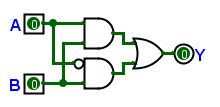
\includegraphics[width=\maxwidth{.95\linewidth}]{gfx/06_01}
	\caption{Simple Circuit For K-Map}
	\label{fig:06_01}
\end{figure}

\begin{align}
  \label{KM:eq:simple_circuit_for_karnaugh_map}
  AB+A'B &= Y
\end{align}

\begin{table}[H]
  \sffamily
  \newcommand{\head}[1]{\textcolor{white}{\textbf{#1}}}    
  \begin{center}
    \rowcolors{2}{gray!10}{white} % Color every other line a light gray
    \begin{tabular}{ccc} 
      \rowcolor{black!75}
      \multicolumn{2}{c}{\head{Inputs}} & \head{Output} \\
      A & B & Y \\
      \hline
      0 & 0 & 0 \\
      0 & 1 & 1 \\
      1 & 0 & 0 \\
      1 & 1 & 1 
    \end{tabular}
  \end{center}
  \caption{Truth Table for Simple Circuit}
  \label{KM:tab:truth_table_simple_circuit}
\end{table}

%****************************************************************
% Karnaugh map For Simple Circuit
%****************************************************************
\begin{figure}[H]
  \caption{Karnaugh map for Simple Circuit}
  \label{KM:tab:k-map_for_simple_circuit}
  \myfloatalign
  \begin{tikzpicture} [circuit logic US, scale=1.00]
  % make all path lines (the node shapes) a little thicker
  \tikzstyle{every path}=[line width=0.50mm]
  
  %********************************************************************
  % Adjust the settings below to display the 1's and rectangles
  %********************************************************************
  % Uncomment the appropriate lines below to insert ones where needed
    \node[] at (1.4,1.5) {\huge $ 0 $}; % 00
    \node[] at (1.4,0.5) {\huge $ 1 $}; % 01
    \node[] at (2.4,1.5) {\huge $ 0 $}; % 02
    \node[] at (2.4,0.5) {\huge $ 1 $}; % 03
  
  % The coords for each cell - this is used as the origin for the solution box
  \coordinate (cell00) at (1.0,3.0); \coordinate (cell01) at (1.0,2.0);
  \coordinate (cell02) at (1.0,0.0); \coordinate (cell03) at (1.0,1.0);
      
  %********************************************************************
  % Shouldn't need to adjust anything below this point - this is just
  % the grid and the minterms.
  %********************************************************************  
  % Text in top-Left cell
  \node[] at (0.35,2.22) { \footnotesize $ \mathsf{ B } $ }; % B
  \node[] at (0.70,2.75) { \footnotesize $ \mathsf{ A } $ }; % A
  
  % Populate the top row header
  % In the following, the foreach lists a location/text pair
  % The the draw line draws the text at each location
  \foreach \loc/\txt in {
    (1.5,2.5)/{0},(2.5,2.5)/{1}
  }
  \draw \loc node{\large $\txt$};
  
  % Populate the header in column one
  \foreach \loc/\txt in { 
    (0.5,1.5)/{0},(0.5,0.5)/{1}
  }
  \draw \loc node{\large $\txt$};
  
  % Populate the minterms
  \foreach \loc/\txt in { 
    (1.75,1.15)/{00} , (2.75,1.15)/{02} , (1.75,0.15)/{01} , (2.75,0.15)/{03} 
    }
  \draw \loc node{ \color{blue!90!black} \footnotesize { $\txt$ }};
  
  % Draw the lines
  \draw
  % Finish drawing the grid
  [step=1.0cm,black,thin] (0,0) grid (3.0,3.0) % The Grid
  (0.0,3.0) -- (1.0,2.0) % Diagonal in the top left cell
  (1.0,2.05) -- (3.0,2.05) % Double line under top header row
  (0.95,0.0) -- (0.95,2.0) % Double line on left of header column one
  ;    
  \end{tikzpicture}
\end{figure}

% Pull Quote - Marginal Note - Sidebar
\marginpar{Karnaugh maps frequently include the minterm numbers in each cell to aid in placing variables.}

First is a circuit diagram, followed by its Boolean equation, truth table, and, finally, Karnaugh map. Think of a Karnaugh map as simply a rearranged truth table; but simplifying a three or four input circuit using a Karnaugh map is much easier and more accurate than with either a truth table or Boolean equation. 

\section{Drawing Two-Variable Karnaugh maps}
\label{KM:sec:drawing_2_variable_karnaugh_maps}

Truth Table \ref{KM:tab:truth_table_with_greek_letters} and Karnaugh map \ref{KM:fig:k-map_with_greek_letters} illustrate the relationship between these two representations of the same circuit using Greek symbols. 

% Table
\begin{table}[H]
  \sffamily
  \newcommand{\head}[1]{\textcolor{white}{\textbf{#1}}}    
  \begin{center}
    \rowcolors{2}{gray!10}{white} % Color every other line a light gray
    \begin{tabular}{ccc} 
      \rowcolor{black!75}
      \multicolumn{2}{c}{\head{Inputs}} & \head{Output} \\
      A & B & Y \\
      \hline
      0 & 0 & $ \alpha $ \\
      0 & 1 & $ \beta $ \\
      1 & 0 & $ \gamma $ \\
      1 & 1 & $ \delta $ 
    \end{tabular}
  \end{center}
  \caption{Truth Table with Greek Letters}
  \label{KM:tab:truth_table_with_greek_letters}
\end{table}

%****************************************************************
% Karnaugh map For 2-Input Circuit With Greek Letters
%****************************************************************
\begin{figure}[H]
  \caption{Karnaugh map With Greek Letters}
  \label{KM:fig:k-map_with_greek_letters}
  \myfloatalign
  \begin{tikzpicture} [circuit logic US, scale=1.00]
  % make all path lines (the node shapes) a little thicker
  \tikzstyle{every path}=[line width=0.50mm]
  
  %********************************************************************
  % Adjust the settings below to display the 1's and rectangles
  %********************************************************************
  % Uncomment the appropriate lines below to insert ones where needed
  \node[] at (1.4,1.5) {\huge $ \alpha $}; % 00
  \node[] at (1.4,0.5) {\huge $ \beta $}; % 01
  \node[] at (2.4,1.5) {\huge $ \gamma $}; % 02
  \node[] at (2.4,0.5) {\huge $ \delta $}; % 03
  
  % The coords for each cell - this is used as the origin for the solution box
  \coordinate (cell00) at (1.0,1.0); \coordinate (cell01) at (1.0,0.0);
  \coordinate (cell02) at (2.0,1.0); \coordinate (cell03) at (2.0,0.0);
  
  %********************************************************************
  % Shouldn't need to adjust anything below this point - this is just
  % the grid and the minterms.
  %********************************************************************  
  % Text in top-Left cell
  \node[] at (0.35,2.22) { \footnotesize $ \mathsf{ B } $ }; % B
  \node[] at (0.70,2.75) { \footnotesize $ \mathsf{ A } $ }; % A
  
  % Populate the top row header
  % In the following, the foreach lists a location/text pair
  % The the draw line draws the text at each location
  \foreach \loc/\txt in {
    (1.5,2.5)/{0},(2.5,2.5)/{1}
  }
  \draw \loc node{\large $\txt$};
  
  % Populate the header in column one
  \foreach \loc/\txt in { 
    (0.5,1.5)/{0},(0.5,0.5)/{1}
  }
  \draw \loc node{\large $\txt$};
  
  % Populate the minterms
  \foreach \loc/\txt in { 
    (1.75,1.15)/{00} , (2.75,1.15)/{02} , (1.75,0.15)/{01} , (2.75,0.15)/{03} 
  }
  \draw \loc node{ \color{blue!90!black} \footnotesize { $\txt$ }};
  
  % Draw the lines
  \draw
  % Finish drawing the grid
  [step=1.0cm,black,thin] (0,0) grid (3.0,3.0) % The Grid
  (0.0,3.0) -- (1.0,2.0) % Diagonal in the top left cell
  (1.0,2.05) -- (3.0,2.05) % Double line under top header row
  (0.95,0.0) -- (0.95,2.0) % Double line on left of header column one
  ;    
  \end{tikzpicture}
\end{figure}

On the Karnaugh map, all of the possible values for input $ A $ are listed across the top of the map and values for input $ B $ are listed down the left side. Thus, to find the output for $ A=0 $; $ B=0 $, look for the cell where those two quantities intersect; which is output $ \alpha $ in the example. It should be clear how all four data squares on the Karnaugh map correspond to their equivalent rows (the minterms) in the Truth Table. 

Truth Table \ref{KM:tab:truth_table_for_2-input_circuit} and Karnaugh map \ref{KM:fig:k-map_for_2_input_circuit} illustrate another example of this relationship.

% Truth Table
\begin{table}[H]
  \sffamily
  \newcommand{\head}[1]{\textcolor{white}{\textbf{#1}}}    
  \begin{center}
    \rowcolors{2}{gray!10}{white} % Color every other line a light gray
    \begin{tabular}{ccc} 
      \rowcolor{black!75}
      \multicolumn{2}{c}{\head{Inputs}} & \head{Output} \\
      A & B & Y \\
      \hline
      0 & 0 & 1 \\
      0 & 1 & 1 \\
      1 & 0 & 0 \\
      1 & 1 & 1 
    \end{tabular}
  \end{center}
  \caption{Truth Table for Two-Input Circuit}
  \label{KM:tab:truth_table_for_2-input_circuit}
\end{table}

%****************************************************************
% Karnaugh map For 2-Input Circuit 
%****************************************************************
\begin{figure}[H]
  \caption{Karnaugh map For Two-Input Circuit}
  \label{KM:fig:k-map_for_2_input_circuit}
  \myfloatalign
  \begin{tikzpicture} [circuit logic US, scale=1.00]
  % make all path lines (the node shapes) a little thicker
  \tikzstyle{every path}=[line width=0.50mm]
  
  %********************************************************************
  % Adjust the settings below to display the 1's and rectangles
  %********************************************************************
  % Uncomment the appropriate lines below to insert ones where needed
  \node[] at (1.4,1.5) {\huge $ 1 $}; % 00
  \node[] at (1.4,0.5) {\huge $ 1 $}; % 01
%  \node[] at (2.4,1.5) {\huge $ 1 $}; % 02
  \node[] at (2.4,0.5) {\huge $ 1 $}; % 03
  
  % The coords for each cell - this is used as the origin for the solution box
  \coordinate (cell00) at (1.0,1.0); \coordinate (cell01) at (1.0,0.0);
  \coordinate (cell02) at (2.0,1.0); \coordinate (cell03) at (2.0,0.0);
  
  %********************************************************************
  % Shouldn't need to adjust anything below this point - this is just
  % the grid and the minterms.
  %********************************************************************  
  % Text in top-Left cell
  \node[] at (0.35,2.22) { \footnotesize $ \mathsf{ B } $ }; % B
  \node[] at (0.70,2.75) { \footnotesize $ \mathsf{ A } $ }; % A
  
  % Populate the top row header
  % In the following, the foreach lists a location/text pair
  % The the draw line draws the text at each location
  \foreach \loc/\txt in {
    (1.5,2.5)/{0},(2.5,2.5)/{1}
  }
  \draw \loc node{\large $\txt$};
  
  % Populate the header in column one
  \foreach \loc/\txt in { 
    (0.5,1.5)/{0},(0.5,0.5)/{1}
  }
  \draw \loc node{\large $\txt$};
  
  % Populate the minterms
  \foreach \loc/\txt in { 
    (1.75,1.15)/{00} , (2.75,1.15)/{02} , (1.75,0.15)/{01} , (2.75,0.15)/{03} 
  }
  \draw \loc node{ \color{blue!90!black} \footnotesize { $\txt$ }};
  
  % Draw the lines
  \draw
  % Finish drawing the grid
  [step=1.0cm,black,thin] (0,0) grid (3.0,3.0) % The Grid
  (0.0,3.0) -- (1.0,2.0) % Diagonal in the top left cell
  (1.0,2.05) -- (3.0,2.05) % Double line under top header row
  (0.95,0.0) -- (0.95,2.0) % Double line on left of header column one
  ;    
  \end{tikzpicture}
\end{figure}
\marginpar{Karnaugh maps usually do not include zeros to decrease the chance for error.}

\section{Drawing Three-Variable Karnaugh maps}
\label{KM:sec:drawing_3-variable_karnaugh_maps}

Consider Equation \ref{KM:eq:karnaugh_map_for_3_variables}.

\begin{align}
  \label{KM:eq:karnaugh_map_for_3_variables}
  ABC'+AB'C+A'B'C &= Y
\end{align}

Table \ref{KM:tab:truth_table_for_3-input_circuit} and Karnaugh map \ref{KM:fig:k-map_for_3-input_circuit} represent this equation.

% Truth Table
\begin{table}[H]
  \sffamily
  \newcommand{\head}[1]{\textcolor{white}{\textbf{#1}}}    
  \begin{center}
    \rowcolors{2}{gray!10}{white} % Color every other line a light gray
    \begin{tabular}{ccccc} 
      \rowcolor{black!75}
      \multicolumn{3}{c}{\head{Inputs}} & \multicolumn{2}{l}{\head{Output}} \\
      A & B & C & Y & minterm \\
      \hline
      0 & 0 & 0 & 0 & 0 \\
      0 & 0 & 1 & 1 & 1 \\
      0 & 1 & 0 & 0 & 2 \\
      0 & 1 & 1 & 0 & 3 \\ 
      1 & 0 & 0 & 0 & 4 \\
      1 & 0 & 1 & 1 & 5 \\
      1 & 1 & 0 & 1 & 6 \\
      1 & 1 & 1 & 0 & 7  
    \end{tabular}
  \end{center}
  \caption{Truth Table for Three-Input Circuit}
  \label{KM:tab:truth_table_for_3-input_circuit}
\end{table}

%****************************************************************
% Karnaugh map For 3-Input Circuit
%****************************************************************
\begin{figure}[H]
  \caption{Karnaugh map for Three-Input Circuit}
  \label{KM:fig:k-map_for_3-input_circuit}
  \myfloatalign
  \begin{tikzpicture} [circuit logic US, scale=1.00]
  % make all path lines (the node shapes) a little thicker
  \tikzstyle{every path}=[line width=0.50mm]
  
  %********************************************************************
  % Adjust the settings below to display the 1's and rectangles
  %********************************************************************
  % Uncomment the appropriate lines below to insert ones where needed
  %  \node[] at (1.4,1.5) {\huge $ 1 $}; % 00
    \node[] at (1.4,0.5) {\huge $ 1 $}; % 01
  %  \node[] at (2.4,1.5) {\huge $ 1 $}; % 02
  %  \node[] at (2.4,0.5) {\huge $ 1 $}; % 03
  %  \node[] at (4.4,1.5) {\huge $ 1 $}; % 04
    \node[] at (4.4,0.5) {\huge $ 1 $}; % 05
    \node[] at (3.4,1.5) {\huge $ 1 $}; % 06
  %  \node[] at (3.4,0.5) {\huge $ 1 $}; % 07
  
  % The coords for each cell - this is used as the origin for the solution box
  \coordinate (cell00) at (1.0,1.0); \coordinate (cell01) at (1.0,0.0);
  \coordinate (cell02) at (2.0,1.0); \coordinate (cell03) at (2.0,0.0);
  
  \coordinate (cell04) at (4.0,1.0); \coordinate (cell05) at (4.0,0.0);
  \coordinate (cell06) at (3.0,1.0); \coordinate (cell07) at (3.0,0.0);
    
  %********************************************************************
  % Shouldn't need to adjust anything below this point - this is just
  % the grid and the minterms.
  %********************************************************************  
  % Text in top-Left cell
  \node[] at (0.35,2.22) { \footnotesize $ \mathsf{ C } $ }; % C
  \node[] at (0.70,2.75) { \footnotesize $ \mathsf{ AB } $ }; % ab
  
  % Populate the top row header
  % In the following, the foreach lists a location/text pair
  % The the draw line draws the text at each location
  \foreach \loc/\txt in {
    (1.5,2.5)/{00},(2.5,2.5)/{01},(3.5,2.5)/{11},(4.5,2.5)/{10}
  }
  \draw \loc node{\large $\txt$};
  
  % Populate the header in column one
  \foreach \loc/\txt in { 
    (0.5,1.5)/{0},(0.5,0.5)/{1}
  }
  \draw \loc node{\large $\txt$};
  
  % Populate the minterms
  \foreach \loc/\txt in { 
    (1.75,1.15)/{00} , (2.75,1.15)/{02} , (3.75,1.15)/{06} , (4.75,1.15)/{04} ,
    (1.75,0.15)/{01} , (2.75,0.15)/{03} , (3.75,0.15)/{07} , (4.75,0.15)/{05} }
  \draw \loc node{ \color{blue!90!black} \footnotesize { $\txt$ }};
  
  % Draw the lines
  \draw
  % Finish drawing the grid
  [step=1.0cm,black,thin] (0,0) grid (5.0,3.0) % The Grid
  (0.0,3.0) -- (1.0,2.0) % Diagonal in the top left cell
  (1.0,2.05) -- (5.0,2.05) % Double line under top header row
  (0.95,0.0) -- (0.95,2.0) % Double line on left of header column one
  ;    
  \end{tikzpicture}
\end{figure}

In Karnaugh map \ref{KM:fig:k-map_for_3-input_circuit} all possible values for inputs $ A $ and $ B $ are listed across the top of the map while input $ C $ is listed down the left side. Therefore, minterm $ m_{05} $, in the lower right corner of the Karnaugh map, is for $ A=1 $; $ B=0 $; $ C=1 $, ($ AB'C $), one of the \emph{True} terms in the original equation. 

\subsection{The Gray Code}
\label{KM:subsec:the_gray_code_for_karnaugh_maps}

It should be noted that the values across the top of the Karnaugh map are not in binary order. Instead, those values are in ``Gray Code'' order. Gray code is essential for a Karnaugh map since the values for adjacent cells must change by only one bit. Constructing the Gray Code for three, four, and five variables is covered on page \pageref{MO:subsub:gray_code}; however, for the Karnaugh maps used in this chapter, it is enough to know the two-bit Gray code: $ 00 $, $ 01 $, $ 11 $, $ 10 $. 

\section{Drawing Four-Variable Karnaugh maps}
\label{KM:sec:drawing_4-variable_karnaugh_maps}

Consider Equation \ref{KM:eq:karnaugh_map_for_4_variables}.

\begin{align}
  \label{KM:eq:karnaugh_map_for_4_variables}
  ABCD'+AB'CD+A'B'CD &= Y
\end{align}

Table \ref{KM:tab:truth_table_for_4-input_circuit} and the Karnaugh map in Figure \ref{KM:fig:kmap_for_four_input_circuit} illustrate this equation.

% Truth Table
\begin{table}[H]
  \sffamily
  \newcommand{\head}[1]{\textcolor{white}{\textbf{#1}}}    
  \begin{center}
    \rowcolors{2}{gray!10}{white} % Color every other line a light gray
    \begin{tabular}{cccccc} 
      \rowcolor{black!75}
      \multicolumn{4}{c}{\head{Inputs}} & \multicolumn{2}{l}{\head{Output}} \\
      A & B & C & D & Y & minterm \\
      \hline
      0 & 0 & 0 & 0 & 0 & 0 \\
      0 & 0 & 0 & 1 & 0 & 1 \\
      0 & 0 & 1 & 0 & 0 & 2 \\
      0 & 0 & 1 & 1 & 1 & 3 \\ 
      0 & 1 & 0 & 0 & 0 & 4 \\
      0 & 1 & 0 & 1 & 0 & 5 \\
      0 & 1 & 1 & 0 & 0 & 6 \\
      1 & 1 & 1 & 1 & 0 & 7 \\
      1 & 0 & 0 & 0 & 0 & 8 \\
      1 & 0 & 0 & 1 & 0 & 9 \\
      1 & 0 & 1 & 0 & 0 & 10 \\
      1 & 0 & 1 & 1 & 1 & 11 \\ 
      1 & 1 & 0 & 0 & 0 & 12 \\
      1 & 1 & 0 & 1 & 0 & 13 \\
      1 & 1 & 1 & 0 & 1 & 14 \\
      1 & 1 & 1 & 1 & 0 & 15  
    \end{tabular}
  \end{center}
  \caption{Truth Table for Four-Input Circuit}
  \label{KM:tab:truth_table_for_4-input_circuit}
\end{table}

%****************************************************************
% Karnaugh map for 4-Input Circuit
%****************************************************************
\begin{figure}[H]
  \caption{K-Map For Four Input Circuit}
  \label{KM:fig:kmap_for_four_input_circuit}
  \myfloatalign
  \begin{tikzpicture} [circuit logic US, scale=1.00]
  % make all path lines (the node shapes) a little thicker
  \tikzstyle{every path}=[line width=0.50mm]
  
  %********************************************************************
  % Adjust the settings below to display the 1's and rectangles
  %********************************************************************
  % Uncomment the appropriate lines below to insert ones where needed
%  \node[] at (1.4,3.5) {\huge $ 1 $}; % 00
%  \node[] at (1.4,2.5) {\huge $ 1 $}; % 01
%  \node[] at (1.4,0.5) {\huge $ 1 $}; % 02
  \node[] at (1.4,1.5) {\huge $ 1 $}; % 03
%  \node[] at (2.4,3.5) {\huge $ 1 $}; % 04
%  \node[] at (2.4,2.5) {\huge $ 1 $}; % 05
%  \node[] at (2.4,0.5) {\huge $ 1 $}; % 06
%  \node[] at (2.4,1.5) {\huge $ 1 $}; % 07
%  \node[] at (4.4,3.5) {\huge $ 1 $}; % 08
%  \node[] at (4.4,2.5) {\huge $ 1 $}; % 09
%  \node[] at (4.4,0.5) {\huge $ 1 $}; % 10
  \node[] at (4.4,1.5) {\huge $ 1 $}; % 11
%  \node[] at (3.4,3.5) {\huge $ 1 $}; % 12
%  \node[] at (3.4,2.5) {\huge $ 1 $}; % 13
  \node[] at (3.4,0.5) {\huge $ 1 $}; % 14
%  \node[] at (3.4,1.5) {\huge $ 1 $}; % 15
  
  % The coords for each cell - this is used as the origin for the solution box
  \coordinate (cell00) at (1.0,3.0); \coordinate (cell01) at (1.0,2.0);
  \coordinate (cell02) at (1.0,0.0); \coordinate (cell03) at (1.0,1.0);

  \coordinate (cell04) at (2.0,3.0); \coordinate (cell05) at (2.0,2.0);
  \coordinate (cell06) at (2.0,0.0); \coordinate (cell07) at (2.0,1.0);

  \coordinate (cell12) at (3.0,3.0); \coordinate (cell13) at (3.0,2.0);
  \coordinate (cell14) at (3.0,0.0); \coordinate (cell15) at (3.0,1.0);

  \coordinate (cell08) at (4.0,3.0); \coordinate (cell09) at (4.0,2.0);
  \coordinate (cell10) at (4.0,0.0); \coordinate (cell11) at (4.0,1.0);
  
  % Horizontal Group
%  \node [draw,
%  color=red!70!black,
%  fill=red!20!white,
%  fill opacity=0.3,
%  minimum height=0.95cm,
%  minimum width=1.95cm, % Adjust to (number of cells) * 1 - 0.95
%  rounded corners,
%  anchor=south west] at (cell02) {}; % Enter left cell minterm
  
  % Vertical Group
%  \node [draw,
%  color=blue!70!black,
%  fill=blue!20!white,
%  fill opacity=0.3,
%  minimum height=1.95cm, % Adjust to (number of cells) * 1 - 0.95
%  minimum width=0.95cm,
%  rounded corners,
%  anchor=south west] at (cell07) {}; % Enter bottom cell minterm
  
  % Single Cell
%  \node [draw,
%  color=green!70!black,
%  fill=green!20!white,
%  fill opacity=0.3,
%  minimum height=0.95cm,
%  minimum width=0.95cm,
%  rounded corners,
%  anchor=south west] at (cell09) {}; % Enter cell minterm
  
  %********************************************************************
  % Shouldn't need to adjust anything below this point - this is just
  % the grid and the minterms.
  %********************************************************************  
  % Text in top-Left cell
  \node[] at (0.35,4.22) { \footnotesize $ \mathsf{ CD } $ }; % cd
  \node[] at (0.70,4.75) { \footnotesize $ \mathsf{ AB } $ }; % ab
  
  % Populate the top row header
  % In the following, the foreach lists a location/text pair
  % The the draw line draws the text at each location
  \foreach \loc/\txt in {
    (1.5,4.5)/{00},(2.5,4.5)/{01},(3.5,4.5)/{11},(4.5,4.5)/{10}
  }
  \draw \loc node{\large $\txt$};
  
  % Populate the header in column one
  \foreach \loc/\txt in { 
    (0.5,3.5)/{00},(0.5,2.5)/{01},(0.5,1.5)/{11},(0.5,0.5)/{10}
  }
  \draw \loc node{\large $\txt$};
  
  % Populate the minterms
  \foreach \loc/\txt in { 
    (1.75,3.15)/{00} , (2.75,3.15)/{04} , (3.75,3.15)/{12} , (4.75,3.15)/{08} ,
    (1.75,2.15)/{01} , (2.75,2.15)/{05} , (3.75,2.15)/{13} , (4.75,2.15)/{09} ,
    (1.75,1.15)/{03} , (2.75,1.15)/{07} , (3.75,1.15)/{15} , (4.75,1.15)/{11} ,
    (1.75,0.15)/{02} , (2.75,0.15)/{06} , (3.75,0.15)/{14} , (4.75,0.15)/{10} }
  \draw \loc node{ \color{blue!90!black} \footnotesize { $\txt$ }};
  
  % Draw the lines
  \draw
  % Finish drawing the grid
  [step=1.0cm,black,thin] (0,0) grid (5.0,5.0) % The Grid
  (0.0,5.0) -- (1.0,4.0) % Diagonal in the top left cell
  (1.0,4.05) -- (5.0,4.05) % Double line under top header row
  (0.95,0.0) -- (0.95,4.0) % Double line on left of header column one
  ;    
  \end{tikzpicture}
\end{figure}

This Karnaugh map is similar to those for two and three variables, but the top row is for the $ A $ and $ B $ inputs while the left column is for the $ C $ and $ D $ inputs. Notice that the values in both the top row and left column use Gray Code sequencing rather than binary counting.

It is easy to indicate the minterms that are \emph{True} on a Karnaugh map if Sigma Notation is available since the numbers following the Sigma sign are the minterms. As an example, Equation \ref{KM:eq:karnaugh_map_when_given_the_sigma_function} creates the Karnaugh map in Figure \ref{KM:fig:kmap_for_sigma_notation}. 

\begin{align}
  \label{KM:eq:karnaugh_map_when_given_the_sigma_function}
  \int{(A,B,C,D)} = \sum(0,1,2,4,5)
\end{align}

%****************************************************************
% Karnaugh map For a Sigma Function
%****************************************************************
\begin{figure}[H]
  \caption{K-Map For Sigma Notation}
  \label{KM:fig:kmap_for_sigma_notation}
  \myfloatalign
  \begin{tikzpicture} [circuit logic US, scale=1.00]
  % make all path lines (the node shapes) a little thicker
  \tikzstyle{every path}=[line width=0.50mm]
  
  %********************************************************************
  % Adjust the settings below to display the 1's and rectangles
  %********************************************************************
  % Uncomment the appropriate lines below to insert ones where needed
    \node[] at (1.4,3.5) {\huge $ 1 $}; % 00
    \node[] at (1.4,2.5) {\huge $ 1 $}; % 01
    \node[] at (1.4,0.5) {\huge $ 1 $}; % 02
  %  \node[] at (1.4,1.5) {\huge $ 1 $}; % 03
    \node[] at (2.4,3.5) {\huge $ 1 $}; % 04
    \node[] at (2.4,2.5) {\huge $ 1 $}; % 05
  %  \node[] at (2.4,0.5) {\huge $ 1 $}; % 06
  %  \node[] at (2.4,1.5) {\huge $ 1 $}; % 07
  %  \node[] at (4.4,3.5) {\huge $ 1 $}; % 08
  %  \node[] at (4.4,2.5) {\huge $ 1 $}; % 09
  %  \node[] at (4.4,0.5) {\huge $ 1 $}; % 10
  %  \node[] at (4.4,1.5) {\huge $ 1 $}; % 11
  %  \node[] at (3.4,3.5) {\huge $ 1 $}; % 12
  %  \node[] at (3.4,2.5) {\huge $ 1 $}; % 13
  %  \node[] at (3.4,0.5) {\huge $ 1 $}; % 14
  %  \node[] at (3.4,1.5) {\huge $ 1 $}; % 15
  
  % The coords for each cell - this is used as the origin for the solution box
  \coordinate (cell00) at (1.0,3.0); \coordinate (cell01) at (1.0,2.0);
  \coordinate (cell02) at (1.0,0.0); \coordinate (cell03) at (1.0,1.0);
  
  \coordinate (cell04) at (2.0,3.0); \coordinate (cell05) at (2.0,2.0);
  \coordinate (cell06) at (2.0,0.0); \coordinate (cell07) at (2.0,1.0);
  
  \coordinate (cell12) at (3.0,3.0); \coordinate (cell13) at (3.0,2.0);
  \coordinate (cell14) at (3.0,0.0); \coordinate (cell15) at (3.0,1.0);
  
  \coordinate (cell08) at (4.0,3.0); \coordinate (cell09) at (4.0,2.0);
  \coordinate (cell10) at (4.0,0.0); \coordinate (cell11) at (4.0,1.0);
  
  % Horizontal Group
  %  \node [draw,
  %  color=red!70!black,
  %  fill=red!20!white,
  %  fill opacity=0.3,
  %  minimum height=0.95cm,
  %  minimum width=1.95cm, % Adjust to (number of cells) * 1 - 0.95
  %  rounded corners,
  %  anchor=south west] at (cell02) {}; % Enter left cell minterm
  
  % Vertical Group
  %  \node [draw,
  %  color=blue!70!black,
  %  fill=blue!20!white,
  %  fill opacity=0.3,
  %  minimum height=1.95cm, % Adjust to (number of cells) * 1 - 0.95
  %  minimum width=0.95cm,
  %  rounded corners,
  %  anchor=south west] at (cell07) {}; % Enter bottom cell minterm
  
  % Single Cell
  %  \node [draw,
  %  color=green!70!black,
  %  fill=green!20!white,
  %  fill opacity=0.3,
  %  minimum height=0.95cm,
  %  minimum width=0.95cm,
  %  rounded corners,
  %  anchor=south west] at (cell09) {}; % Enter cell minterm
  
  %********************************************************************
  % Shouldn't need to adjust anything below this point - this is just
  % the grid and the minterms.
  %********************************************************************  
  % Text in top-Left cell
  \node[] at (0.35,4.22) { \footnotesize $ \mathsf{ CD } $ }; % cd
  \node[] at (0.70,4.75) { \footnotesize $ \mathsf{ AB } $ }; % ab
  
  % Populate the top row header
  % In the following, the foreach lists a location/text pair
  % The the draw line draws the text at each location
  \foreach \loc/\txt in {
    (1.5,4.5)/{00},(2.5,4.5)/{01},(3.5,4.5)/{11},(4.5,4.5)/{10}
  }
  \draw \loc node{\large $\txt$};
  
  % Populate the header in column one
  \foreach \loc/\txt in { 
    (0.5,3.5)/{00},(0.5,2.5)/{01},(0.5,1.5)/{11},(0.5,0.5)/{10}
  }
  \draw \loc node{\large $\txt$};
  
  % Populate the minterms
  \foreach \loc/\txt in { 
    (1.75,3.15)/{00} , (2.75,3.15)/{04} , (3.75,3.15)/{12} , (4.75,3.15)/{08} ,
    (1.75,2.15)/{01} , (2.75,2.15)/{05} , (3.75,2.15)/{13} , (4.75,2.15)/{09} ,
    (1.75,1.15)/{03} , (2.75,1.15)/{07} , (3.75,1.15)/{15} , (4.75,1.15)/{11} ,
    (1.75,0.15)/{02} , (2.75,0.15)/{06} , (3.75,0.15)/{14} , (4.75,0.15)/{10} }
  \draw \loc node{ \color{blue!90!black} \footnotesize { $\txt$ }};
  
  % Draw the lines
  \draw
  % Finish drawing the grid
  [step=1.0cm,black,thin] (0,0) grid (5.0,5.0) % The Grid
  (0.0,5.0) -- (1.0,4.0) % Diagonal in the top left cell
  (1.0,4.05) -- (5.0,4.05) % Double line under top header row
  (0.95,0.0) -- (0.95,4.0) % Double line on left of header column one
  ;    
  \end{tikzpicture}
\end{figure}

It is also possible to map values if the circuit is represented in Pi notation; but remember that maxterms indicate where zeros are placed on the Karnaugh map and the simplified circuit would actually be the inverse of the needed circuit. As an example, Equation \ref{KM:eq:karnaugh_map_when_given_the_pi_function} creates the Karnaugh map at Figure \ref{KM:fig:kmap_for_pi_notation}. 

\begin{align}
  \label{KM:eq:karnaugh_map_when_given_the_pi_function}
  \int{(A,B,C,D)} = \prod(8,9,12,13)
\end{align}

%****************************************************************
% Karnaugh map for a PI Function
%****************************************************************
\begin{figure}[H]
  \caption{K-Map For PI Notation}
  \label{KM:fig:kmap_for_pi_notation}
  \myfloatalign
  \begin{tikzpicture} [circuit logic US, scale=1.00]
  % make all path lines (the node shapes) a little thicker
  \tikzstyle{every path}=[line width=0.50mm]
  
  %********************************************************************
  % Adjust the settings below to display the 1's and rectangles
  %********************************************************************
  % Uncomment the appropriate lines below to insert ones where needed
  %  \node[] at (1.4,3.5) {\huge $ 0 $}; % 00
  %  \node[] at (1.4,2.5) {\huge $ 0 $}; % 01
  %  \node[] at (1.4,0.5) {\huge $ 0 $}; % 02
  %  \node[] at (1.4,1.5) {\huge $ 0 $}; % 03
  %  \node[] at (2.4,3.5) {\huge $ 0 $}; % 04
  %  \node[] at (2.4,2.5) {\huge $ 0 $}; % 05
  %  \node[] at (2.4,0.5) {\huge $ 0 $}; % 06
  %  \node[] at (2.4,1.5) {\huge $ 0 $}; % 07
    \node[] at (4.4,3.5) {\huge $ 0 $}; % 08
    \node[] at (4.4,2.5) {\huge $ 0 $}; % 09
  %  \node[] at (4.4,0.5) {\huge $ 0 $}; % 10
  %  \node[] at (4.4,1.5) {\huge $ 0 $}; % 11
    \node[] at (3.4,3.5) {\huge $ 0 $}; % 12
    \node[] at (3.4,2.5) {\huge $ 0 $}; % 13
  %  \node[] at (3.4,0.5) {\huge $ 0 $}; % 14
  %  \node[] at (3.4,1.5) {\huge $ 0 $}; % 15
  
  % The coords for each cell - this is used as the origin for the solution box
  \coordinate (cell00) at (1.0,3.0); \coordinate (cell01) at (1.0,2.0);
  \coordinate (cell02) at (1.0,0.0); \coordinate (cell03) at (1.0,1.0);
  
  \coordinate (cell04) at (2.0,3.0); \coordinate (cell05) at (2.0,2.0);
  \coordinate (cell06) at (2.0,0.0); \coordinate (cell07) at (2.0,1.0);
  
  \coordinate (cell12) at (3.0,3.0); \coordinate (cell13) at (3.0,2.0);
  \coordinate (cell14) at (3.0,0.0); \coordinate (cell15) at (3.0,1.0);
  
  \coordinate (cell08) at (4.0,3.0); \coordinate (cell09) at (4.0,2.0);
  \coordinate (cell10) at (4.0,0.0); \coordinate (cell11) at (4.0,1.0);
  
  % Horizontal Group
  %  \node [draw,
  %  color=red!70!black,
  %  fill=red!20!white,
  %  fill opacity=0.3,
  %  minimum height=0.95cm,
  %  minimum width=1.95cm, % Adjust to (number of cells) * 1 - 0.95
  %  rounded corners,
  %  anchor=south west] at (cell02) {}; % Enter left cell minterm
  
  % Vertical Group
  %  \node [draw,
  %  color=blue!70!black,
  %  fill=blue!20!white,
  %  fill opacity=0.3,
  %  minimum height=1.95cm, % Adjust to (number of cells) * 1 - 0.95
  %  minimum width=0.95cm,
  %  rounded corners,
  %  anchor=south west] at (cell07) {}; % Enter bottom cell minterm
  
  % Single Cell
  %  \node [draw,
  %  color=green!70!black,
  %  fill=green!20!white,
  %  fill opacity=0.3,
  %  minimum height=0.95cm,
  %  minimum width=0.95cm,
  %  rounded corners,
  %  anchor=south west] at (cell09) {}; % Enter cell minterm
  
  %********************************************************************
  % Shouldn't need to adjust anything below this point - this is just
  % the grid and the minterms.
  %********************************************************************  
  % Text in top-Left cell
  \node[] at (0.35,4.22) { \footnotesize $ \mathsf{ CD } $ }; % cd
  \node[] at (0.70,4.75) { \footnotesize $ \mathsf{ AB } $ }; % ab
  
  % Populate the top row header
  % In the following, the foreach lists a location/text pair
  % The the draw line draws the text at each location
  \foreach \loc/\txt in {
    (1.5,4.5)/{00},(2.5,4.5)/{01},(3.5,4.5)/{11},(4.5,4.5)/{10}
  }
  \draw \loc node{\large $\txt$};
  
  % Populate the header in column one
  \foreach \loc/\txt in { 
    (0.5,3.5)/{00},(0.5,2.5)/{01},(0.5,1.5)/{11},(0.5,0.5)/{10}
  }
  \draw \loc node{\large $\txt$};
  
  % Populate the minterms
  \foreach \loc/\txt in { 
    (1.75,3.15)/{00} , (2.75,3.15)/{04} , (3.75,3.15)/{12} , (4.75,3.15)/{08} ,
    (1.75,2.15)/{01} , (2.75,2.15)/{05} , (3.75,2.15)/{13} , (4.75,2.15)/{09} ,
    (1.75,1.15)/{03} , (2.75,1.15)/{07} , (3.75,1.15)/{15} , (4.75,1.15)/{11} ,
    (1.75,0.15)/{02} , (2.75,0.15)/{06} , (3.75,0.15)/{14} , (4.75,0.15)/{10} }
  \draw \loc node{ \color{blue!90!black} \footnotesize { $\txt$ }};
  
  % Draw the lines
  \draw
  % Finish drawing the grid
  [step=1.0cm,black,thin] (0,0) grid (5.0,5.0) % The Grid
  (0.0,5.0) -- (1.0,4.0) % Diagonal in the top left cell
  (1.0,4.05) -- (5.0,4.05) % Double line under top header row
  (0.95,0.0) -- (0.95,4.0) % Double line on left of header column one
  ;    
  \end{tikzpicture}
\end{figure}

To simplify this map, the designer could place ones in all of the empty cells and then simplify the ``ones'' circuit using the techniques explained below. Alternatively, the designer could also simplify the map by combining the zeros as if they were ones, and then finding the DeMorgan inverse (page  \pageref{BF:sec:demorgans_theorem}) of that simplification. As an example, the maxterm Karnaugh map above would simplify to $ \overline{AC'} $, and the DeMorgan equivalent for that is $ A'+C $, which is the minterm version of the simplified circuit.

\section{Simplifying Groups of Two}
\label{KM:sec:simplifying_groups_of_two}

To simplify a Boolean equation using a Karnaugh map, start by creating the Karnaugh map, indicating the input variable combinations that lead to a \emph{True} output for the circuit. Equations \ref{KM:eq:simplifying_4-input_equations_groups_of_two} and \ref{KM:eq:sigma_notation_solving_k-map_groups_of_two} are for the same circuit and the Karnaugh map in Figure \ref{KM:fig:k-map_for_groups_of_two_ex_1} was built from these equations. 

\begin{align}
  \label{KM:eq:simplifying_4-input_equations_groups_of_two}
  A'B'C'D'+A'BC'D'+A'BCD+AB'CD'+AB'CD
\end{align}

\begin{align}
  \label{KM:eq:sigma_notation_solving_k-map_groups_of_two}
  \int{(A,B,C,D)} = \sum(0,4,7,10,11)
\end{align}

%****************************************************************
% Karnaugh map For Groups of 2, Example 1
%****************************************************************
\begin{figure}[H]
  \caption{K-Map for Groups of Two: Ex 1}
  \label{KM:fig:k-map_for_groups_of_two_ex_1}
  \myfloatalign
  \begin{tikzpicture} [circuit logic US, scale=1.00]
  % make all path lines (the node shapes) a little thicker
  \tikzstyle{every path}=[line width=0.50mm]
  
  %********************************************************************
  % Adjust the settings below to display the 1's and rectangles
  %********************************************************************
  % Uncomment the appropriate lines below to insert ones where needed
    \node[] at (1.4,3.5) {\huge $ 1 $}; % 00
  %  \node[] at (1.4,2.5) {\huge $ 1 $}; % 01
  %  \node[] at (1.4,0.5) {\huge $ 1 $}; % 02
  %  \node[] at (1.4,1.5) {\huge $ 1 $}; % 03
    \node[] at (2.4,3.5) {\huge $ 1 $}; % 04
  %  \node[] at (2.4,2.5) {\huge $ 1 $}; % 05
  %  \node[] at (2.4,0.5) {\huge $ 1 $}; % 06
    \node[] at (2.4,1.5) {\huge $ 1 $}; % 07
  %  \node[] at (4.4,3.5) {\huge $ 1 $}; % 08
  %  \node[] at (4.4,2.5) {\huge $ 1 $}; % 09
    \node[] at (4.4,0.5) {\huge $ 1 $}; % 10
    \node[] at (4.4,1.5) {\huge $ 1 $}; % 11
  %  \node[] at (3.4,3.5) {\huge $ 1 $}; % 12
  %  \node[] at (3.4,2.5) {\huge $ 1 $}; % 13
  %  \node[] at (3.4,0.5) {\huge $ 1 $}; % 14
  %  \node[] at (3.4,1.5) {\huge $ 1 $}; % 15
  
  % The coords for each cell - this is used as the origin for the solution box
  \coordinate (cell00) at (1.0,3.0); \coordinate (cell01) at (1.0,2.0);
  \coordinate (cell02) at (1.0,0.0); \coordinate (cell03) at (1.0,1.0);
  
  \coordinate (cell04) at (2.0,3.0); \coordinate (cell05) at (2.0,2.0);
  \coordinate (cell06) at (2.0,0.0); \coordinate (cell07) at (2.0,1.0);
  
  \coordinate (cell12) at (3.0,3.0); \coordinate (cell13) at (3.0,2.0);
  \coordinate (cell14) at (3.0,0.0); \coordinate (cell15) at (3.0,1.0);
  
  \coordinate (cell08) at (4.0,3.0); \coordinate (cell09) at (4.0,2.0);
  \coordinate (cell10) at (4.0,0.0); \coordinate (cell11) at (4.0,1.0);
  
  % Horizontal Group
  %  \node [draw,
  %  color=red!70!black,
  %  fill=red!20!white,
  %  fill opacity=0.3,
  %  minimum height=0.95cm,
  %  minimum width=1.95cm, % Adjust to (number of cells) * 1 - 0.95
  %  rounded corners,
  %  anchor=south west] at (cell02) {}; % Enter left cell minterm
  
  % Vertical Group
  %  \node [draw,
  %  color=blue!70!black,
  %  fill=blue!20!white,
  %  fill opacity=0.3,
  %  minimum height=1.95cm, % Adjust to (number of cells) * 1 - 0.95
  %  minimum width=0.95cm,
  %  rounded corners,
  %  anchor=south west] at (cell07) {}; % Enter bottom cell minterm
  
  % Single Cell
  %  \node [draw,
  %  color=green!70!black,
  %  fill=green!20!white,
  %  fill opacity=0.3,
  %  minimum height=0.95cm,
  %  minimum width=0.95cm,
  %  rounded corners,
  %  anchor=south west] at (cell09) {}; % Enter cell minterm
  
  %********************************************************************
  % Shouldn't need to adjust anything below this point - this is just
  % the grid and the minterms.
  %********************************************************************  
  % Text in top-Left cell
  \node[] at (0.35,4.22) { \footnotesize $ \mathsf{ CD } $ }; % cd
  \node[] at (0.70,4.75) { \footnotesize $ \mathsf{ AB } $ }; % ab
  
  % Populate the top row header
  % In the following, the foreach lists a location/text pair
  % The the draw line draws the text at each location
  \foreach \loc/\txt in {
    (1.5,4.5)/{00},(2.5,4.5)/{01},(3.5,4.5)/{11},(4.5,4.5)/{10}
  }
  \draw \loc node{\large $\txt$};
  
  % Populate the header in column one
  \foreach \loc/\txt in { 
    (0.5,3.5)/{00},(0.5,2.5)/{01},(0.5,1.5)/{11},(0.5,0.5)/{10}
  }
  \draw \loc node{\large $\txt$};
  
  % Populate the minterms
  \foreach \loc/\txt in { 
    (1.75,3.15)/{00} , (2.75,3.15)/{04} , (3.75,3.15)/{12} , (4.75,3.15)/{08} ,
    (1.75,2.15)/{01} , (2.75,2.15)/{05} , (3.75,2.15)/{13} , (4.75,2.15)/{09} ,
    (1.75,1.15)/{03} , (2.75,1.15)/{07} , (3.75,1.15)/{15} , (4.75,1.15)/{11} ,
    (1.75,0.15)/{02} , (2.75,0.15)/{06} , (3.75,0.15)/{14} , (4.75,0.15)/{10} }
  \draw \loc node{ \color{blue!90!black} \footnotesize { $\txt$ }};
  
  % Draw the lines
  \draw
  % Finish drawing the grid
  [step=1.0cm,black,thin] (0,0) grid (5.0,5.0) % The Grid
  (0.0,5.0) -- (1.0,4.0) % Diagonal in the top left cell
  (1.0,4.05) -- (5.0,4.05) % Double line under top header row
  (0.95,0.0) -- (0.95,4.0) % Double line on left of header column one
  ;    
  \end{tikzpicture}
\end{figure}

Once the \emph{True} outputs are indicated on the Karnaugh map, mark any groups of ones that are adjacent to each other, either horizontally or vertically (but not diagonally). Also, mark any ones that are ``left over'' and are not adjacent to any other ones, as illustrated in the Karnaugh map in Figure \ref{KM:fig:kmap_solving_groups_of_two_ex_1}. 

%****************************************************************
% Karnaugh map For Groups of 2, Example 1, Simplified
%****************************************************************
\begin{figure}[H]
  \caption{K-Map for Groups of Two: Ex 1, Solved}
  \label{KM:fig:k-map_for_groups_of_two_ex_1_solved}
  \myfloatalign
  \begin{tikzpicture} [circuit logic US, scale=1.00]
  % make all path lines (the node shapes) a little thicker
  \tikzstyle{every path}=[line width=0.50mm]
  
  %********************************************************************
  % Adjust the settings below to display the 1's and rectangles
  %********************************************************************
  % Uncomment the appropriate lines below to insert ones where needed
  \node[] at (1.4,3.5) {\huge $ 1 $}; % 00
  %  \node[] at (1.4,2.5) {\huge $ 1 $}; % 01
  %  \node[] at (1.4,0.5) {\huge $ 1 $}; % 02
  %  \node[] at (1.4,1.5) {\huge $ 1 $}; % 03
  \node[] at (2.4,3.5) {\huge $ 1 $}; % 04
  %  \node[] at (2.4,2.5) {\huge $ 1 $}; % 05
  %  \node[] at (2.4,0.5) {\huge $ 1 $}; % 06
  \node[] at (2.4,1.5) {\huge $ 1 $}; % 07
  %  \node[] at (4.4,3.5) {\huge $ 1 $}; % 08
  %  \node[] at (4.4,2.5) {\huge $ 1 $}; % 09
  \node[] at (4.4,0.5) {\huge $ 1 $}; % 10
  \node[] at (4.4,1.5) {\huge $ 1 $}; % 11
  %  \node[] at (3.4,3.5) {\huge $ 1 $}; % 12
  %  \node[] at (3.4,2.5) {\huge $ 1 $}; % 13
  %  \node[] at (3.4,0.5) {\huge $ 1 $}; % 14
  %  \node[] at (3.4,1.5) {\huge $ 1 $}; % 15
  
  % The coords for each cell - this is used as the origin for the solution box
  \coordinate (cell00) at (1.0,3.0); \coordinate (cell01) at (1.0,2.0);
  \coordinate (cell02) at (1.0,0.0); \coordinate (cell03) at (1.0,1.0);
  
  \coordinate (cell04) at (2.0,3.0); \coordinate (cell05) at (2.0,2.0);
  \coordinate (cell06) at (2.0,0.0); \coordinate (cell07) at (2.0,1.0);
  
  \coordinate (cell12) at (3.0,3.0); \coordinate (cell13) at (3.0,2.0);
  \coordinate (cell14) at (3.0,0.0); \coordinate (cell15) at (3.0,1.0);
  
  \coordinate (cell08) at (4.0,3.0); \coordinate (cell09) at (4.0,2.0);
  \coordinate (cell10) at (4.0,0.0); \coordinate (cell11) at (4.0,1.0);
  
  % Horizontal Group
    \node [draw,
    color=red!70!black,
    fill=red!20!white,
    fill opacity=0.3,
    minimum height=0.95cm,
    minimum width=1.95cm, % Adjust to (number of cells) * 1 - 0.95
    rounded corners,
    anchor=south west] at (cell00) {}; % Enter left cell minterm
  
  % Vertical Group
    \node [draw,
    color=blue!70!black,
    fill=blue!20!white,
    fill opacity=0.3,
    minimum height=1.95cm, % Adjust to (number of cells) * 1 - 0.95
    minimum width=0.95cm,
    rounded corners,
    anchor=south west] at (cell10) {}; % Enter bottom cell minterm
  
  % Single Cell
    \node [draw,
    color=green!70!black,
    fill=green!20!white,
    fill opacity=0.3,
    minimum height=0.95cm,
    minimum width=0.95cm,
    rounded corners,
    anchor=south west] at (cell07) {}; % Enter cell minterm
  
  %********************************************************************
  % Shouldn't need to adjust anything below this point - this is just
  % the grid and the minterms.
  %********************************************************************  
  % Text in top-Left cell
  \node[] at (0.35,4.22) { \footnotesize $ \mathsf{ CD } $ }; % cd
  \node[] at (0.70,4.75) { \footnotesize $ \mathsf{ AB } $ }; % ab
  
  % Populate the top row header
  % In the following, the foreach lists a location/text pair
  % The the draw line draws the text at each location
  \foreach \loc/\txt in {
    (1.5,4.5)/{00},(2.5,4.5)/{01},(3.5,4.5)/{11},(4.5,4.5)/{10}
  }
  \draw \loc node{\large $\txt$};
  
  % Populate the header in column one
  \foreach \loc/\txt in { 
    (0.5,3.5)/{00},(0.5,2.5)/{01},(0.5,1.5)/{11},(0.5,0.5)/{10}
  }
  \draw \loc node{\large $\txt$};
  
  % Populate the minterms
  \foreach \loc/\txt in { 
    (1.75,3.15)/{00} , (2.75,3.15)/{04} , (3.75,3.15)/{12} , (4.75,3.15)/{08} ,
    (1.75,2.15)/{01} , (2.75,2.15)/{05} , (3.75,2.15)/{13} , (4.75,2.15)/{09} ,
    (1.75,1.15)/{03} , (2.75,1.15)/{07} , (3.75,1.15)/{15} , (4.75,1.15)/{11} ,
    (1.75,0.15)/{02} , (2.75,0.15)/{06} , (3.75,0.15)/{14} , (4.75,0.15)/{10} }
  \draw \loc node{ \color{blue!90!black} \footnotesize { $\txt$ }};
  
  % Draw the lines
  \draw
  % Finish drawing the grid
  [step=1.0cm,black,thin] (0,0) grid (5.0,5.0) % The Grid
  (0.0,5.0) -- (1.0,4.0) % Diagonal in the top left cell
  (1.0,4.05) -- (5.0,4.05) % Double line under top header row
  (0.95,0.0) -- (0.95,4.0) % Double line on left of header column one
  ;    
  \end{tikzpicture}
\end{figure}

Notice the group in the top-left corner (minterms $ 00 $ and $ 04 $). This group includes the following two input combinations: $ A'B'C'D' + A'BC'D' $. In this expression, the $ B $ and $ B' $ terms can be removed by the Complement Property (page \pageref{BF:subsec:complement}); so this group reduces to $ A'C'D' $. To simplify this expression by inspecting the Karnaugh map, notice that the variable $ A $ is zero for both of these minterms; therefore, $ A' $ must be part of the final expression. In the same way, variables $ C $ and $ D $ are zero for both terms; therefore, $ C'D' $ must be part of the final expression. Since variable $ B $ changes it can be ignored when forming the simplified expression.

The group in the lower-right corner (minterms $ 10 $ and $ 11 $) includes the following two input variable combinations: $ AB'CD + AB'CD' $. The $ D $ and $ D' $ terms can be removed by the Complement Property; so this group simplifies to $ AB'C $. Again, inspecting these two terms would reveal that the variables $ AB'C $ do not change between the two terms, so they must appear in the final expression. 

Minterm $ 07 $, the lone term indicated in column two, cannot be reduced since it is not adjacent to any other ones. Therefore, it must go into the simplified equation unchanged: $ A'BCD $. 

When finished, the original equation reduces to Equation \ref{KM:eq:sigma_notation_solving_k-map_groups_of_two_solution}.

\begin{align}
  \label{KM:eq:sigma_notation_solving_k-map_groups_of_two_solution}
  A'C'D'+AB'C+A'BCD
\end{align}

Using a Karnaugh map, the circuit was simplified from four four-input \textsf{AND} gates to two three-input \textsf{AND} gates and one four-input \textsf{AND} gate. 

The various ones on a Karnaugh map are called the \emph{Implicants} of the solution. These are the algebraic products that are necessary to ``imply'' (or bring about) the final simplification of the circuit. When an implicant cannot be grouped with any others, or when two or more implicants are grouped together, they are called \emph{Prime Implicants}. The three groups ($ A'C'D' $, $ AB'C $, and $ A'BCD $) found by analyzing the Karnaugh map above are the prime implicants for this equation. When prime implicants are a necessary part of the final simplified equation, and they are not subsumed by any other implicants, they are called \emph{Essential Prime Implicants}. For the simple example given above, all of the prime implicants are essential; however, more complex Karnaugh maps may have numerous prime implicants that are subsumed by other implicants; thus, are not essential. There are examples of these types of maps later in this chapter. 

A second example is illustrated in Equation \ref{KM:eq:simplifying_4-input_equations_groups_of_two_ex_2} and the Karnaugh map in Figure \ref{KM:fig:kmap_solving_groups_of_two_ex_2}.

\begin{align}
  \label{KM:eq:simplifying_4-input_equations_groups_of_two_ex_2}
  &A'B'C'D+A'B'CD+A'BCD'+ \\
  \nonumber
  &ABC'D+ABCD'+AB'C'D'=Y
\end{align}

\begin{align}
  \label{KM:eq:sigma_notation_solving_k-map_groups_of_two_ex_2}
  \int{(A,B,C,D)} = \sum(1,3,6,8,13,14)
\end{align}

%****************************************************************
% Karnaugh map For Groups of 2, Example 2
%****************************************************************
\begin{figure}[H]
  \caption{K-Map Solving Groups of Two: Example 2}
  \label{KM:fig:kmap_solving_groups_of_two_ex_2}
  \myfloatalign
  \begin{tikzpicture} [circuit logic US, scale=1.00]
  % make all path lines (the node shapes) a little thicker
  \tikzstyle{every path}=[line width=0.50mm]
  
  %********************************************************************
  % Adjust the settings below to display the 1's and rectangles
  %********************************************************************
  % Uncomment the appropriate lines below to insert ones where needed
  %  \node[] at (1.4,3.5) {\huge $ 1 $}; % 00
    \node[] at (1.4,2.5) {\huge $ 1 $}; % 01
  %  \node[] at (1.4,0.5) {\huge $ 1 $}; % 02
    \node[] at (1.4,1.5) {\huge $ 1 $}; % 03
  %  \node[] at (2.4,3.5) {\huge $ 1 $}; % 04
  %  \node[] at (2.4,2.5) {\huge $ 1 $}; % 05
    \node[] at (2.4,0.5) {\huge $ 1 $}; % 06
  %  \node[] at (2.4,1.5) {\huge $ 1 $}; % 07
    \node[] at (4.4,3.5) {\huge $ 1 $}; % 08
  %  \node[] at (4.4,2.5) {\huge $ 1 $}; % 09
  %  \node[] at (4.4,0.5) {\huge $ 1 $}; % 10
  %  \node[] at (4.4,1.5) {\huge $ 1 $}; % 11
  %  \node[] at (3.4,3.5) {\huge $ 1 $}; % 12
    \node[] at (3.4,2.5) {\huge $ 1 $}; % 13
    \node[] at (3.4,0.5) {\huge $ 1 $}; % 14
  %  \node[] at (3.4,1.5) {\huge $ 1 $}; % 15
  
  % The coords for each cell - this is used as the origin for the solution box
  \coordinate (cell00) at (1.0,3.0); \coordinate (cell01) at (1.0,2.0);
  \coordinate (cell02) at (1.0,0.0); \coordinate (cell03) at (1.0,1.0);
  
  \coordinate (cell04) at (2.0,3.0); \coordinate (cell05) at (2.0,2.0);
  \coordinate (cell06) at (2.0,0.0); \coordinate (cell07) at (2.0,1.0);
  
  \coordinate (cell12) at (3.0,3.0); \coordinate (cell13) at (3.0,2.0);
  \coordinate (cell14) at (3.0,0.0); \coordinate (cell15) at (3.0,1.0);
  
  \coordinate (cell08) at (4.0,3.0); \coordinate (cell09) at (4.0,2.0);
  \coordinate (cell10) at (4.0,0.0); \coordinate (cell11) at (4.0,1.0);
  
  % Horizontal Group
    \node [draw,
    color=red!70!black,
    fill=red!20!white,
    fill opacity=0.3,
    minimum height=0.95cm,
    minimum width=1.95cm, % Adjust to (number of cells) * 1 - 0.95
    rounded corners,
    anchor=south west] at (cell06) {}; % Enter left cell minterm
  
  % Vertical Group
    \node [draw,
    color=blue!70!black,
    fill=blue!20!white,
    fill opacity=0.3,
    minimum height=1.95cm, % Adjust to (number of cells) * 1 - 0.95
    minimum width=0.95cm,
  %  rounded corners,
    anchor=south west] at (cell03) {}; % Enter bottom cell minterm
  
  % Single Cell
    \node [draw,
    color=green!70!black,
    fill=green!20!white,
    fill opacity=0.3,
    minimum height=0.95cm,
    minimum width=0.95cm,
    rounded corners,
    anchor=south west] at (cell13) {}; % Enter cell minterm

  % Single Cell
    \node [draw,
    color=green!70!black,
    fill=green!20!white,
    fill opacity=0.3,
    minimum height=0.95cm,
    minimum width=0.95cm,
    rounded corners,
    anchor=south west] at (cell08) {}; % Enter cell minterm
  
  %********************************************************************
  % Shouldn't need to adjust anything below this point - this is just
  % the grid and the minterms.
  %********************************************************************  
  % Text in top-Left cell
  \node[] at (0.35,4.22) { \footnotesize $ \mathsf{ CD } $ }; % cd
  \node[] at (0.70,4.75) { \footnotesize $ \mathsf{ AB } $ }; % ab
  
  % Populate the top row header
  % In the following, the foreach lists a location/text pair
  % The the draw line draws the text at each location
  \foreach \loc/\txt in {
    (1.5,4.5)/{00},(2.5,4.5)/{01},(3.5,4.5)/{11},(4.5,4.5)/{10}
  }
  \draw \loc node{\large $\txt$};
  
  % Populate the header in column one
  \foreach \loc/\txt in { 
    (0.5,3.5)/{00},(0.5,2.5)/{01},(0.5,1.5)/{11},(0.5,0.5)/{10}
  }
  \draw \loc node{\large $\txt$};
  
  % Populate the minterms
  \foreach \loc/\txt in { 
    (1.75,3.15)/{00} , (2.75,3.15)/{04} , (3.75,3.15)/{12} , (4.75,3.15)/{08} ,
    (1.75,2.15)/{01} , (2.75,2.15)/{05} , (3.75,2.15)/{13} , (4.75,2.15)/{09} ,
    (1.75,1.15)/{03} , (2.75,1.15)/{07} , (3.75,1.15)/{15} , (4.75,1.15)/{11} ,
    (1.75,0.15)/{02} , (2.75,0.15)/{06} , (3.75,0.15)/{14} , (4.75,0.15)/{10} }
  \draw \loc node{ \color{blue!90!black} \footnotesize { $\txt$ }};
  
  % Draw the lines
  \draw
  % Finish drawing the grid
  [step=1.0cm,black,thin] (0,0) grid (5.0,5.0) % The Grid
  (0.0,5.0) -- (1.0,4.0) % Diagonal in the top left cell
  (1.0,4.05) -- (5.0,4.05) % Double line under top header row
  (0.95,0.0) -- (0.95,4.0) % Double line on left of header column one
  ;    
  \end{tikzpicture}
\end{figure}

All groups of adjacent ones have been marked, so this circuit can be simplified by looking for groups of two. Starting with minterms $ 01 $ and $ 03 $, $ A'B'C'D + A'B'CD $ simplifies to $ A'B'D $. Minterms $ 06 $ and $ 14 $ simplifies to $ BCD' $. The other two marked minterms are not adjacent to any others, so they cannot be simplified. Each of the marked terms are prime implicants; and since they are not subsumed by any other implicants, they are essential prime implicants. Equation \ref{KM:eq:simplifying_4-input_equations_groups_of_two_ex_2_solution} is the simplified solution.

\begin{align}
  \label{KM:eq:simplifying_4-input_equations_groups_of_two_ex_2_solution}
  &ABC'D+AB'C'D'+A'B'D+BCD' = Y
\end{align}

\section{Simplifying Larger Groups}
\label{KM:sec:simplifying_larger_groups}

When simplifying Karnaugh maps, it is most efficient to find groups of $ 16 $, $ 8 $, $ 4 $, and $ 2 $ adjacent ones, in that order. In general, the larger the group, the simpler the expression becomes; so one large group is preferable to two smaller groups. However, remember that any group can only use ones that are adjacent along a horizontal or vertical line, not diagonal. 

\subsection{Groups of 16}
\label{KM:subsec:groups_of_16}

Groups of $ 16 $ reduce to a constant output of one. This is because if a circuit is built such that every possible combination of four inputs yields a \emph{True} output, then the circuit is unnecessary and can be replaced by a wire. There is no example Karnaugh map posted here to illustrate a circuit like this because if every cell in a Karnaugh map contains a one, then the circuit is unnecessary. By the same token, any Karnaugh map that contains only zeros indicates that the circuit would never output a \emph{True} condition so the circuit is unnecessary.

\subsection{Groups of Eight}
\label{KM:subsec:groups_of_8}

Groups of eight simplifies to a single output variable. Consider the Karnaugh map in Figure \ref{KM:fig:kmap_solving_groups_of_8}. 

%****************************************************************
% Karnaugh map For Groups of 8
%****************************************************************
\begin{figure}[H]
  \caption{K-Map Solving Groups of 8}
  \label{KM:fig:kmap_solving_groups_of_8}
  \myfloatalign
  \begin{tikzpicture} [circuit logic US, scale=1.00]
  % make all path lines (the node shapes) a little thicker
  \tikzstyle{every path}=[line width=0.50mm]
  
  %********************************************************************
  % Adjust the settings below to display the 1's and rectangles
  %********************************************************************
  % Uncomment the appropriate lines below to insert ones where needed
  %  \node[] at (1.4,3.5) {\huge $ 1 $}; % 00
    \node[] at (1.4,2.5) {\huge $ 1 $}; % 01
  %  \node[] at (1.4,0.5) {\huge $ 1 $}; % 02
    \node[] at (1.4,1.5) {\huge $ 1 $}; % 03
  %  \node[] at (2.4,3.5) {\huge $ 1 $}; % 04
    \node[] at (2.4,2.5) {\huge $ 1 $}; % 05
  %  \node[] at (2.4,0.5) {\huge $ 1 $}; % 06
    \node[] at (2.4,1.5) {\huge $ 1 $}; % 07
  %  \node[] at (4.4,3.5) {\huge $ 1 $}; % 08
    \node[] at (4.4,2.5) {\huge $ 1 $}; % 09
  %  \node[] at (4.4,0.5) {\huge $ 1 $}; % 10
    \node[] at (4.4,1.5) {\huge $ 1 $}; % 11
  %  \node[] at (3.4,3.5) {\huge $ 1 $}; % 12
    \node[] at (3.4,2.5) {\huge $ 1 $}; % 13
  %  \node[] at (3.4,0.5) {\huge $ 1 $}; % 14
    \node[] at (3.4,1.5) {\huge $ 1 $}; % 15
  
  % The coords for each cell - this is used as the origin for the solution box
  \coordinate (cell00) at (1.0,3.0); \coordinate (cell01) at (1.0,2.0);
  \coordinate (cell02) at (1.0,0.0); \coordinate (cell03) at (1.0,1.0);
  
  \coordinate (cell04) at (2.0,3.0); \coordinate (cell05) at (2.0,2.0);
  \coordinate (cell06) at (2.0,0.0); \coordinate (cell07) at (2.0,1.0);
  
  \coordinate (cell12) at (3.0,3.0); \coordinate (cell13) at (3.0,2.0);
  \coordinate (cell14) at (3.0,0.0); \coordinate (cell15) at (3.0,1.0);
  
  \coordinate (cell08) at (4.0,3.0); \coordinate (cell09) at (4.0,2.0);
  \coordinate (cell10) at (4.0,0.0); \coordinate (cell11) at (4.0,1.0);
  
  % Horizontal Group
    \node [draw,
    color=red!70!black,
    fill=red!20!white,
    fill opacity=0.3,
    minimum height=1.95cm,
    minimum width=3.95cm, % Adjust to (number of cells) * 1 - 0.95
    rounded corners,
    anchor=south west] at (cell03) {}; % Enter left cell minterm
  
  % Vertical Group
  %  \node [draw,
  %  color=blue!70!black,
  %  fill=blue!20!white,
  %  fill opacity=0.3,
  %  minimum height=1.95cm, % Adjust to (number of cells) * 1 - 0.95
  %  minimum width=0.95cm,
  %  rounded corners,
  %  anchor=south west] at (cell07) {}; % Enter bottom cell minterm
  
  % Single Cell
  %  \node [draw,
  %  color=green!70!black,
  %  fill=green!20!white,
  %  fill opacity=0.3,
  %  minimum height=0.95cm,
  %  minimum width=0.95cm,
  %  rounded corners,
  %  anchor=south west] at (cell09) {}; % Enter cell minterm
  
  %********************************************************************
  % Shouldn't need to adjust anything below this point - this is just
  % the grid and the minterms.
  %********************************************************************  
  % Text in top-Left cell
  \node[] at (0.35,4.22) { \footnotesize $ \mathsf{ CD } $ }; % cd
  \node[] at (0.70,4.75) { \footnotesize $ \mathsf{ AB } $ }; % ab
  
  % Populate the top row header
  % In the following, the foreach lists a location/text pair
  % The the draw line draws the text at each location
  \foreach \loc/\txt in {
    (1.5,4.5)/{00},(2.5,4.5)/{01},(3.5,4.5)/{11},(4.5,4.5)/{10}
  }
  \draw \loc node{\large $\txt$};
  
  % Populate the header in column one
  \foreach \loc/\txt in { 
    (0.5,3.5)/{00},(0.5,2.5)/{01},(0.5,1.5)/{11},(0.5,0.5)/{10}
  }
  \draw \loc node{\large $\txt$};
  
  % Populate the minterms
  \foreach \loc/\txt in { 
    (1.75,3.15)/{00} , (2.75,3.15)/{04} , (3.75,3.15)/{12} , (4.75,3.15)/{08} ,
    (1.75,2.15)/{01} , (2.75,2.15)/{05} , (3.75,2.15)/{13} , (4.75,2.15)/{09} ,
    (1.75,1.15)/{03} , (2.75,1.15)/{07} , (3.75,1.15)/{15} , (4.75,1.15)/{11} ,
    (1.75,0.15)/{02} , (2.75,0.15)/{06} , (3.75,0.15)/{14} , (4.75,0.15)/{10} }
  \draw \loc node{ \color{blue!90!black} \footnotesize { $\txt$ }};
  
  % Draw the lines
  \draw
  % Finish drawing the grid
  [step=1.0cm,black,thin] (0,0) grid (5.0,5.0) % The Grid
  (0.0,5.0) -- (1.0,4.0) % Diagonal in the top left cell
  (1.0,4.05) -- (5.0,4.05) % Double line under top header row
  (0.95,0.0) -- (0.95,4.0) % Double line on left of header column one
  ;    
  \end{tikzpicture}
\end{figure}

The expression for row two is: $ A'B'C'D + A'BC'D + ABC'D + AB'C'D $. The term $ C'D $ is constant in this group, while $ A $ and $ B $ change, so this one line would simplify to $ C'D $. The expression for row three is: $ A'B'CD + A'BCD + ABCD + AB'CD $. The term $ CD $ is constant in this group, so this one line would simplify to $ CD $. Then, if the two rows are combined: $ C'D + CD $, $ C $ and $ C' $ are dropped by the complement property and the circuit simplifies to $ D $. To put this another way, since the only term in this group of eight that never changes is $ D $, then Equation \ref{KM:eq:simplifying_4-input_equations_groups_of_eight_solution} is the simplified solution.

\begin{align}
  \label{KM:eq:simplifying_4-input_equations_groups_of_eight_solution}
  D = Y
\end{align}

This Karnaugh map also provides a good example of prime implicants that are not essential. Consider row two of the map. Minterms $ 01 $ and $ 05 $ form a Prime Implicant for this circuit since it is a group of two; however, that group was subsumed by the group of eight that was formed with the next row. Since every cell in the group of two is also present in the group of eight, then the group of two is not essential to the final circuit simplification. While this may seem to be rather obvious, it is important to remember that frequently implicants are formed that are not essential and they can be ignored. This concept will come up again when using the Quine-McCluskey Simplification method on page \pageref{ASM:sec:quine-mccluskey_simplification_method}. 

\subsection{Groups of Four}
\label{KM:subsec:groups_of_4}

Groups of four can form as a single row, a single column, or a square. In any case, the four cells will simplify to a two-variable expression. Consider the Karnaugh map in Figure \ref{KM:fig:kmap_solving_groups_of_four_ex_1} 

%****************************************************************
% Karnaugh map For Groups of 4, Example 1
%****************************************************************
\begin{figure}[H]
  \caption{K-Map Solving Groups of Four, Example 1}
  \label{KM:fig:kmap_solving_groups_of_four_ex_1}
  \myfloatalign
  \begin{tikzpicture} [circuit logic US, scale=1.00]
  % make all path lines (the node shapes) a little thicker
  \tikzstyle{every path}=[line width=0.50mm]
  
  %********************************************************************
  % Adjust the settings below to display the 1's and rectangles
  %********************************************************************
  % Uncomment the appropriate lines below to insert ones where needed
  %  \node[] at (1.4,3.5) {\huge $ 1 $}; % 00
    \node[] at (1.4,2.5) {\huge $ 1 $}; % 01
  %  \node[] at (1.4,0.5) {\huge $ 1 $}; % 02
  %  \node[] at (1.4,1.5) {\huge $ 1 $}; % 03
  %  \node[] at (2.4,3.5) {\huge $ 1 $}; % 04
    \node[] at (2.4,2.5) {\huge $ 1 $}; % 05
  %  \node[] at (2.4,0.5) {\huge $ 1 $}; % 06
  %  \node[] at (2.4,1.5) {\huge $ 1 $}; % 07
  %  \node[] at (4.4,3.5) {\huge $ 1 $}; % 08
    \node[] at (4.4,2.5) {\huge $ 1 $}; % 09
  %  \node[] at (4.4,0.5) {\huge $ 1 $}; % 10
  %  \node[] at (4.4,1.5) {\huge $ 1 $}; % 11
  %  \node[] at (3.4,3.5) {\huge $ 1 $}; % 12
    \node[] at (3.4,2.5) {\huge $ 1 $}; % 13
  %  \node[] at (3.4,0.5) {\huge $ 1 $}; % 14
  %  \node[] at (3.4,1.5) {\huge $ 1 $}; % 15
  
  % The coords for each cell - this is used as the origin for the solution box
  \coordinate (cell00) at (1.0,3.0); \coordinate (cell01) at (1.0,2.0);
  \coordinate (cell02) at (1.0,0.0); \coordinate (cell03) at (1.0,1.0);
  
  \coordinate (cell04) at (2.0,3.0); \coordinate (cell05) at (2.0,2.0);
  \coordinate (cell06) at (2.0,0.0); \coordinate (cell07) at (2.0,1.0);
  
  \coordinate (cell12) at (3.0,3.0); \coordinate (cell13) at (3.0,2.0);
  \coordinate (cell14) at (3.0,0.0); \coordinate (cell15) at (3.0,1.0);
  
  \coordinate (cell08) at (4.0,3.0); \coordinate (cell09) at (4.0,2.0);
  \coordinate (cell10) at (4.0,0.0); \coordinate (cell11) at (4.0,1.0);
  
  % Horizontal Group
    \node [draw,
    color=red!70!black,
    fill=red!20!white,
    fill opacity=0.3,
    minimum height=0.95cm,
    minimum width=3.95cm, % Adjust to (number of cells) * 1 - 0.95
    rounded corners,
    anchor=south west] at (cell01) {}; % Enter left cell minterm
  
  % Vertical Group
  %  \node [draw,
  %  color=blue!70!black,
  %  fill=blue!20!white,
  %  fill opacity=0.3,
  %  minimum height=1.95cm, % Adjust to (number of cells) * 1 - 0.95
  %  minimum width=0.95cm,
  %  rounded corners,
  %  anchor=south west] at (cell07) {}; % Enter bottom cell minterm
  
  % Single Cell
  %  \node [draw,
  %  color=green!70!black,
  %  fill=green!20!white,
  %  fill opacity=0.3,
  %  minimum height=0.95cm,
  %  minimum width=0.95cm,
  %  rounded corners,
  %  anchor=south west] at (cell09) {}; % Enter cell minterm
  
  %********************************************************************
  % Shouldn't need to adjust anything below this point - this is just
  % the grid and the minterms.
  %********************************************************************  
  % Text in top-Left cell
  \node[] at (0.35,4.22) { \footnotesize $ \mathsf{ CD } $ }; % cd
  \node[] at (0.70,4.75) { \footnotesize $ \mathsf{ AB } $ }; % ab
  
  % Populate the top row header
  % In the following, the foreach lists a location/text pair
  % The the draw line draws the text at each location
  \foreach \loc/\txt in {
    (1.5,4.5)/{00},(2.5,4.5)/{01},(3.5,4.5)/{11},(4.5,4.5)/{10}
  }
  \draw \loc node{\large $\txt$};
  
  % Populate the header in column one
  \foreach \loc/\txt in { 
    (0.5,3.5)/{00},(0.5,2.5)/{01},(0.5,1.5)/{11},(0.5,0.5)/{10}
  }
  \draw \loc node{\large $\txt$};
  
  % Populate the minterms
  \foreach \loc/\txt in { 
    (1.75,3.15)/{00} , (2.75,3.15)/{04} , (3.75,3.15)/{12} , (4.75,3.15)/{08} ,
    (1.75,2.15)/{01} , (2.75,2.15)/{05} , (3.75,2.15)/{13} , (4.75,2.15)/{09} ,
    (1.75,1.15)/{03} , (2.75,1.15)/{07} , (3.75,1.15)/{15} , (4.75,1.15)/{11} ,
    (1.75,0.15)/{02} , (2.75,0.15)/{06} , (3.75,0.15)/{14} , (4.75,0.15)/{10} }
  \draw \loc node{ \color{blue!90!black} \footnotesize { $\txt$ }};
  
  % Draw the lines
  \draw
  % Finish drawing the grid
  [step=1.0cm,black,thin] (0,0) grid (5.0,5.0) % The Grid
  (0.0,5.0) -- (1.0,4.0) % Diagonal in the top left cell
  (1.0,4.05) -- (5.0,4.05) % Double line under top header row
  (0.95,0.0) -- (0.95,4.0) % Double line on left of header column one
  ;    
  \end{tikzpicture}
\end{figure}

Since the $ A $ and $ B $ variables can be removed due to the Complement Property, Equation \ref{KM:eq:solving_groups_of_four_ex_1} shows the simplified solution. 

\begin{align}
  \label{KM:eq:solving_groups_of_four_ex_1}
  C'D = Y
\end{align}

The Karnaugh map in Figure \ref{KM:fig:kmap_solving_groups_of_four_ex_2} is a second example.

%****************************************************************
% Karnaugh map For Groups of 4, Example 2
%****************************************************************
\begin{figure}[H]
  \caption{K-Map Solving Groups of Four, Example 2}
  \label{KM:fig:kmap_solving_groups_of_four_ex_2}
  \myfloatalign
  \begin{tikzpicture} [circuit logic US, scale=1.00]
  % make all path lines (the node shapes) a little thicker
  \tikzstyle{every path}=[line width=0.50mm]
  
  %********************************************************************
  % Adjust the settings below to display the 1's and rectangles
  %********************************************************************
  % Uncomment the appropriate lines below to insert ones where needed
  %  \node[] at (1.4,3.5) {\huge $ 1 $}; % 00
  %  \node[] at (1.4,2.5) {\huge $ 1 $}; % 01
  %  \node[] at (1.4,0.5) {\huge $ 1 $}; % 02
  %  \node[] at (1.4,1.5) {\huge $ 1 $}; % 03
  %  \node[] at (2.4,3.5) {\huge $ 1 $}; % 04
  %  \node[] at (2.4,2.5) {\huge $ 1 $}; % 05
  %  \node[] at (2.4,0.5) {\huge $ 1 $}; % 06
  %  \node[] at (2.4,1.5) {\huge $ 1 $}; % 07
  %  \node[] at (4.4,3.5) {\huge $ 1 $}; % 08
  %  \node[] at (4.4,2.5) {\huge $ 1 $}; % 09
  %  \node[] at (4.4,0.5) {\huge $ 1 $}; % 10
  %  \node[] at (4.4,1.5) {\huge $ 1 $}; % 11
    \node[] at (3.4,3.5) {\huge $ 1 $}; % 12
    \node[] at (3.4,2.5) {\huge $ 1 $}; % 13
    \node[] at (3.4,0.5) {\huge $ 1 $}; % 14
    \node[] at (3.4,1.5) {\huge $ 1 $}; % 15
  
  % The coords for each cell - this is used as the origin for the solution box
  \coordinate (cell00) at (1.0,3.0); \coordinate (cell01) at (1.0,2.0);
  \coordinate (cell02) at (1.0,0.0); \coordinate (cell03) at (1.0,1.0);
  
  \coordinate (cell04) at (2.0,3.0); \coordinate (cell05) at (2.0,2.0);
  \coordinate (cell06) at (2.0,0.0); \coordinate (cell07) at (2.0,1.0);
  
  \coordinate (cell12) at (3.0,3.0); \coordinate (cell13) at (3.0,2.0);
  \coordinate (cell14) at (3.0,0.0); \coordinate (cell15) at (3.0,1.0);
  
  \coordinate (cell08) at (4.0,3.0); \coordinate (cell09) at (4.0,2.0);
  \coordinate (cell10) at (4.0,0.0); \coordinate (cell11) at (4.0,1.0);
  
  % Horizontal Group
  %  \node [draw,
  %  color=red!70!black,
  %  fill=red!20!white,
  %  fill opacity=0.3,
  %  minimum height=0.95cm,
  %  minimum width=1.95cm, % Adjust to (number of cells) * 1 - 0.95
  %  rounded corners,
  %  anchor=south west] at (cell02) {}; % Enter left cell minterm
  
  % Vertical Group
    \node [draw,
    color=blue!70!black,
    fill=blue!20!white,
    fill opacity=0.3,
    minimum height=3.95cm, % Adjust to (number of cells) * 1 - 0.95
    minimum width=0.95cm,
    rounded corners,
    anchor=south west] at (cell14) {}; % Enter bottom cell minterm
  
  % Single Cell
  %  \node [draw,
  %  color=green!70!black,
  %  fill=green!20!white,
  %  fill opacity=0.3,
  %  minimum height=0.95cm,
  %  minimum width=0.95cm,
  %  rounded corners,
  %  anchor=south west] at (cell09) {}; % Enter cell minterm
  
  %********************************************************************
  % Shouldn't need to adjust anything below this point - this is just
  % the grid and the minterms.
  %********************************************************************  
  % Text in top-Left cell
  \node[] at (0.35,4.22) { \footnotesize $ \mathsf{ CD } $ }; % cd
  \node[] at (0.70,4.75) { \footnotesize $ \mathsf{ AB } $ }; % ab
  
  % Populate the top row header
  % In the following, the foreach lists a location/text pair
  % The the draw line draws the text at each location
  \foreach \loc/\txt in {
    (1.5,4.5)/{00},(2.5,4.5)/{01},(3.5,4.5)/{11},(4.5,4.5)/{10}
  }
  \draw \loc node{\large $\txt$};
  
  % Populate the header in column one
  \foreach \loc/\txt in { 
    (0.5,3.5)/{00},(0.5,2.5)/{01},(0.5,1.5)/{11},(0.5,0.5)/{10}
  }
  \draw \loc node{\large $\txt$};
  
  % Populate the minterms
  \foreach \loc/\txt in { 
    (1.75,3.15)/{00} , (2.75,3.15)/{04} , (3.75,3.15)/{12} , (4.75,3.15)/{08} ,
    (1.75,2.15)/{01} , (2.75,2.15)/{05} , (3.75,2.15)/{13} , (4.75,2.15)/{09} ,
    (1.75,1.15)/{03} , (2.75,1.15)/{07} , (3.75,1.15)/{15} , (4.75,1.15)/{11} ,
    (1.75,0.15)/{02} , (2.75,0.15)/{06} , (3.75,0.15)/{14} , (4.75,0.15)/{10} }
  \draw \loc node{ \color{blue!90!black} \footnotesize { $\txt$ }};
  
  % Draw the lines
  \draw
  % Finish drawing the grid
  [step=1.0cm,black,thin] (0,0) grid (5.0,5.0) % The Grid
  (0.0,5.0) -- (1.0,4.0) % Diagonal in the top left cell
  (1.0,4.05) -- (5.0,4.05) % Double line under top header row
  (0.95,0.0) -- (0.95,4.0) % Double line on left of header column one
  ;    
  \end{tikzpicture}
\end{figure}

Since the $ C $ and $ D $ variables can be removed due to the Complement Property, Equation \ref{KM:eq:simplifying_4-input_equations_groups_of_four_ex_2_solution} shows the simplified circuit. 

\begin{align}
  \label{KM:eq:simplifying_4-input_equations_groups_of_four_ex_2_solution}
  AB = Y
\end{align}

The Karnaugh map in Figure \ref{KM:fig:kmap_solving_groups_of_four_ex_3} is an example of a group of four that forms a square.

%****************************************************************
% Karnaugh map For Groups of 4, Example 3
%****************************************************************
\begin{figure}[H]
  \caption{K-Map Solving Groups of Four, Example 3}
  \label{KM:fig:kmap_solving_groups_of_four_ex_3}
  \myfloatalign
  \begin{tikzpicture} [circuit logic US, scale=1.00]
  % make all path lines (the node shapes) a little thicker
  \tikzstyle{every path}=[line width=0.50mm]
  
  %********************************************************************
  % Adjust the settings below to display the 1's and rectangles
  %********************************************************************
  % Uncomment the appropriate lines below to insert ones where needed
  %  \node[] at (1.4,3.5) {\huge $ 1 $}; % 00
    \node[] at (1.4,2.5) {\huge $ 1 $}; % 01
  %  \node[] at (1.4,0.5) {\huge $ 1 $}; % 02
    \node[] at (1.4,1.5) {\huge $ 1 $}; % 03
  %  \node[] at (2.4,3.5) {\huge $ 1 $}; % 04
    \node[] at (2.4,2.5) {\huge $ 1 $}; % 05
  %  \node[] at (2.4,0.5) {\huge $ 1 $}; % 06
    \node[] at (2.4,1.5) {\huge $ 1 $}; % 07
  %  \node[] at (4.4,3.5) {\huge $ 1 $}; % 08
  %  \node[] at (4.4,2.5) {\huge $ 1 $}; % 09
  %  \node[] at (4.4,0.5) {\huge $ 1 $}; % 10
  %  \node[] at (4.4,1.5) {\huge $ 1 $}; % 11
  %  \node[] at (3.4,3.5) {\huge $ 1 $}; % 12
  %  \node[] at (3.4,2.5) {\huge $ 1 $}; % 13
  %  \node[] at (3.4,0.5) {\huge $ 1 $}; % 14
  %  \node[] at (3.4,1.5) {\huge $ 1 $}; % 15
  
  % The coords for each cell - this is used as the origin for the solution box
  \coordinate (cell00) at (1.0,3.0); \coordinate (cell01) at (1.0,2.0);
  \coordinate (cell02) at (1.0,0.0); \coordinate (cell03) at (1.0,1.0);
  
  \coordinate (cell04) at (2.0,3.0); \coordinate (cell05) at (2.0,2.0);
  \coordinate (cell06) at (2.0,0.0); \coordinate (cell07) at (2.0,1.0);
  
  \coordinate (cell12) at (3.0,3.0); \coordinate (cell13) at (3.0,2.0);
  \coordinate (cell14) at (3.0,0.0); \coordinate (cell15) at (3.0,1.0);
  
  \coordinate (cell08) at (4.0,3.0); \coordinate (cell09) at (4.0,2.0);
  \coordinate (cell10) at (4.0,0.0); \coordinate (cell11) at (4.0,1.0);
  
  % Horizontal Group
  %  \node [draw,
  %  color=red!70!black,
  %  fill=red!20!white,
  %  fill opacity=0.3,
  %  minimum height=0.95cm,
  %  minimum width=1.95cm, % Adjust to (number of cells) * 1 - 0.95
  %  rounded corners,
  %  anchor=south west] at (cell02) {}; % Enter left cell minterm
  
  % Vertical Group
  %  \node [draw,
  %  color=blue!70!black,
  %  fill=blue!20!white,
  %  fill opacity=0.3,
  %  minimum height=1.95cm, % Adjust to (number of cells) * 1 - 0.95
  %  minimum width=0.95cm,
  %  rounded corners,
  %  anchor=south west] at (cell07) {}; % Enter bottom cell minterm
  
  % Single Cell
    \node [draw,
    color=green!70!black,
    fill=green!20!white,
    fill opacity=0.3,
    minimum height=1.95cm,
    minimum width=1.95cm,
    rounded corners,
    anchor=south west] at (cell03) {}; % Enter cell minterm
  
  %********************************************************************
  % Shouldn't need to adjust anything below this point - this is just
  % the grid and the minterms.
  %********************************************************************  
  % Text in top-Left cell
  \node[] at (0.35,4.22) { \footnotesize $ \mathsf{ CD } $ }; % cd
  \node[] at (0.70,4.75) { \footnotesize $ \mathsf{ AB } $ }; % ab
  
  % Populate the top row header
  % In the following, the foreach lists a location/text pair
  % The the draw line draws the text at each location
  \foreach \loc/\txt in {
    (1.5,4.5)/{00},(2.5,4.5)/{01},(3.5,4.5)/{11},(4.5,4.5)/{10}
  }
  \draw \loc node{\large $\txt$};
  
  % Populate the header in column one
  \foreach \loc/\txt in { 
    (0.5,3.5)/{00},(0.5,2.5)/{01},(0.5,1.5)/{11},(0.5,0.5)/{10}
  }
  \draw \loc node{\large $\txt$};
  
  % Populate the minterms
  \foreach \loc/\txt in { 
    (1.75,3.15)/{00} , (2.75,3.15)/{04} , (3.75,3.15)/{12} , (4.75,3.15)/{08} ,
    (1.75,2.15)/{01} , (2.75,2.15)/{05} , (3.75,2.15)/{13} , (4.75,2.15)/{09} ,
    (1.75,1.15)/{03} , (2.75,1.15)/{07} , (3.75,1.15)/{15} , (4.75,1.15)/{11} ,
    (1.75,0.15)/{02} , (2.75,0.15)/{06} , (3.75,0.15)/{14} , (4.75,0.15)/{10} }
  \draw \loc node{ \color{blue!90!black} \footnotesize { $\txt$ }};
  
  % Draw the lines
  \draw
  % Finish drawing the grid
  [step=1.0cm,black,thin] (0,0) grid (5.0,5.0) % The Grid
  (0.0,5.0) -- (1.0,4.0) % Diagonal in the top left cell
  (1.0,4.05) -- (5.0,4.05) % Double line under top header row
  (0.95,0.0) -- (0.95,4.0) % Double line on left of header column one
  ;    
  \end{tikzpicture}
\end{figure}

Since the $ B $ and $ C $ variables can be removed due to the Complement Property, Equation \ref{KM:eq:simplifying_4-input_equations_groups_of_four_ex_3_solution} shows the simplified circuit. 

\begin{align}
  \label{KM:eq:simplifying_4-input_equations_groups_of_four_ex_3_solution}
  A'D = Y
\end{align}

\subsection{Groups of Two}
\label{KM:subsec:groups_of_2}

Groups of two will simplify to a three-variable expression. The Karnaugh map in Figure \ref{KM:fig:kmap_solving_groups_of_two_ex_1} is one example of a group of two. 

%****************************************************************
% Karnaugh map For Groups of 2, Example 1
%****************************************************************
\begin{figure}[H]
  \caption{K-Map Solving Groups of Two, Example 1}
  \label{KM:fig:kmap_solving_groups_of_two_ex_1}
  \myfloatalign
  \begin{tikzpicture} [circuit logic US, scale=1.00]
  % make all path lines (the node shapes) a little thicker
  \tikzstyle{every path}=[line width=0.50mm]
  
  %********************************************************************
  % Adjust the settings below to display the 1's and rectangles
  %********************************************************************
  % Uncomment the appropriate lines below to insert ones where needed
  %  \node[] at (1.4,3.5) {\huge $ 1 $}; % 00
  %  \node[] at (1.4,2.5) {\huge $ 1 $}; % 01
  %  \node[] at (1.4,0.5) {\huge $ 1 $}; % 02
  %  \node[] at (1.4,1.5) {\huge $ 1 $}; % 03
  %  \node[] at (2.4,3.5) {\huge $ 1 $}; % 04
  %  \node[] at (2.4,2.5) {\huge $ 1 $}; % 05
  %  \node[] at (2.4,0.5) {\huge $ 1 $}; % 06
  %  \node[] at (2.4,1.5) {\huge $ 1 $}; % 07
  %  \node[] at (4.4,3.5) {\huge $ 1 $}; % 08
    \node[] at (4.4,2.5) {\huge $ 1 $}; % 09
  %  \node[] at (4.4,0.5) {\huge $ 1 $}; % 10
    \node[] at (4.4,1.5) {\huge $ 1 $}; % 11
  %  \node[] at (3.4,3.5) {\huge $ 1 $}; % 12
  %  \node[] at (3.4,2.5) {\huge $ 1 $}; % 13
  %  \node[] at (3.4,0.5) {\huge $ 1 $}; % 14
  %  \node[] at (3.4,1.5) {\huge $ 1 $}; % 15
  
  % The coords for each cell - this is used as the origin for the solution box
  \coordinate (cell00) at (1.0,3.0); \coordinate (cell01) at (1.0,2.0);
  \coordinate (cell02) at (1.0,0.0); \coordinate (cell03) at (1.0,1.0);
  
  \coordinate (cell04) at (2.0,3.0); \coordinate (cell05) at (2.0,2.0);
  \coordinate (cell06) at (2.0,0.0); \coordinate (cell07) at (2.0,1.0);
  
  \coordinate (cell12) at (3.0,3.0); \coordinate (cell13) at (3.0,2.0);
  \coordinate (cell14) at (3.0,0.0); \coordinate (cell15) at (3.0,1.0);
  
  \coordinate (cell08) at (4.0,3.0); \coordinate (cell09) at (4.0,2.0);
  \coordinate (cell10) at (4.0,0.0); \coordinate (cell11) at (4.0,1.0);
  
  % Horizontal Group
  %  \node [draw,
  %  color=red!70!black,
  %  fill=red!20!white,
  %  fill opacity=0.3,
  %  minimum height=0.95cm,
  %  minimum width=1.95cm, % Adjust to (number of cells) * 1 - 0.95
  %  rounded corners,
  %  anchor=south west] at (cell02) {}; % Enter left cell minterm
  
  % Vertical Group
    \node [draw,
    color=blue!70!black,
    fill=blue!20!white,
    fill opacity=0.3,
    minimum height=1.95cm, % Adjust to (number of cells) * 1 - 0.95
    minimum width=0.95cm,
    rounded corners,
    anchor=south west] at (cell11) {}; % Enter bottom cell minterm
  
  % Single Cell
  %  \node [draw,
  %  color=green!70!black,
  %  fill=green!20!white,
  %  fill opacity=0.3,
  %  minimum height=0.95cm,
  %  minimum width=0.95cm,
  %  rounded corners,
  %  anchor=south west] at (cell09) {}; % Enter cell minterm
  
  %********************************************************************
  % Shouldn't need to adjust anything below this point - this is just
  % the grid and the minterms.
  %********************************************************************  
  % Text in top-Left cell
  \node[] at (0.35,4.22) { \footnotesize $ \mathsf{ CD } $ }; % cd
  \node[] at (0.70,4.75) { \footnotesize $ \mathsf{ AB } $ }; % ab
  
  % Populate the top row header
  % In the following, the foreach lists a location/text pair
  % The the draw line draws the text at each location
  \foreach \loc/\txt in {
    (1.5,4.5)/{00},(2.5,4.5)/{01},(3.5,4.5)/{11},(4.5,4.5)/{10}
  }
  \draw \loc node{\large $\txt$};
  
  % Populate the header in column one
  \foreach \loc/\txt in { 
    (0.5,3.5)/{00},(0.5,2.5)/{01},(0.5,1.5)/{11},(0.5,0.5)/{10}
  }
  \draw \loc node{\large $\txt$};
  
  % Populate the minterms
  \foreach \loc/\txt in { 
    (1.75,3.15)/{00} , (2.75,3.15)/{04} , (3.75,3.15)/{12} , (4.75,3.15)/{08} ,
    (1.75,2.15)/{01} , (2.75,2.15)/{05} , (3.75,2.15)/{13} , (4.75,2.15)/{09} ,
    (1.75,1.15)/{03} , (2.75,1.15)/{07} , (3.75,1.15)/{15} , (4.75,1.15)/{11} ,
    (1.75,0.15)/{02} , (2.75,0.15)/{06} , (3.75,0.15)/{14} , (4.75,0.15)/{10} }
  \draw \loc node{ \color{blue!90!black} \footnotesize { $\txt$ }};
  
  % Draw the lines
  \draw
  % Finish drawing the grid
  [step=1.0cm,black,thin] (0,0) grid (5.0,5.0) % The Grid
  (0.0,5.0) -- (1.0,4.0) % Diagonal in the top left cell
  (1.0,4.05) -- (5.0,4.05) % Double line under top header row
  (0.95,0.0) -- (0.95,4.0) % Double line on left of header column one
  ;    
  \end{tikzpicture}
\end{figure}

Since $ C $ is the only variable that can be removed due to the Complement Property, the above circuit simplifies to Equation \ref{KM:eq:simplifying_4-input_equations_groups_of_two_ex_1_solution}.

\begin{align}
  \label{KM:eq:simplifying_4-input_equations_groups_of_two_ex_1_solution}
  AB'D = Y
\end{align}

As a second example, consider the Karnaugh map in Figure \ref{KM:fig:kmap_solving_groups_of_two_ex_2}.

%****************************************************************
% Karnaugh map For Groups of 2, Example 2
%****************************************************************
\begin{figure}[H]
  \caption{K-Map Solving Groups of Two, Example 2}
  \label{KM:fig:kmap_solving_groups_of_two_ex_2}
  \myfloatalign
  \begin{tikzpicture} [circuit logic US, scale=1.00]
  % make all path lines (the node shapes) a little thicker
  \tikzstyle{every path}=[line width=0.50mm]
  
  %********************************************************************
  % Adjust the settings below to display the 1's and rectangles
  %********************************************************************
  % Uncomment the appropriate lines below to insert ones where needed
  %  \node[] at (1.4,3.5) {\huge $ 1 $}; % 00
  %  \node[] at (1.4,2.5) {\huge $ 1 $}; % 01
  %  \node[] at (1.4,0.5) {\huge $ 1 $}; % 02
  %  \node[] at (1.4,1.5) {\huge $ 1 $}; % 03
  %  \node[] at (2.4,3.5) {\huge $ 1 $}; % 04
  %  \node[] at (2.4,2.5) {\huge $ 1 $}; % 05
  %  \node[] at (2.4,0.5) {\huge $ 1 $}; % 06
    \node[] at (2.4,1.5) {\huge $ 1 $}; % 07
  %  \node[] at (4.4,3.5) {\huge $ 1 $}; % 08
  %  \node[] at (4.4,2.5) {\huge $ 1 $}; % 09
  %  \node[] at (4.4,0.5) {\huge $ 1 $}; % 10
  %  \node[] at (4.4,1.5) {\huge $ 1 $}; % 11
  %  \node[] at (3.4,3.5) {\huge $ 1 $}; % 12
  %  \node[] at (3.4,2.5) {\huge $ 1 $}; % 13
  %  \node[] at (3.4,0.5) {\huge $ 1 $}; % 14
    \node[] at (3.4,1.5) {\huge $ 1 $}; % 15
  
  % The coords for each cell - this is used as the origin for the solution box
  \coordinate (cell00) at (1.0,3.0); \coordinate (cell01) at (1.0,2.0);
  \coordinate (cell02) at (1.0,0.0); \coordinate (cell03) at (1.0,1.0);
  
  \coordinate (cell04) at (2.0,3.0); \coordinate (cell05) at (2.0,2.0);
  \coordinate (cell06) at (2.0,0.0); \coordinate (cell07) at (2.0,1.0);
  
  \coordinate (cell12) at (3.0,3.0); \coordinate (cell13) at (3.0,2.0);
  \coordinate (cell14) at (3.0,0.0); \coordinate (cell15) at (3.0,1.0);
  
  \coordinate (cell08) at (4.0,3.0); \coordinate (cell09) at (4.0,2.0);
  \coordinate (cell10) at (4.0,0.0); \coordinate (cell11) at (4.0,1.0);
  
  % Horizontal Group
    \node [draw,
    color=red!70!black,
    fill=red!20!white,
    fill opacity=0.3,
    minimum height=0.95cm,
    minimum width=1.95cm, % Adjust to (number of cells) * 1 - 0.95
    rounded corners,
    anchor=south west] at (cell07) {}; % Enter left cell minterm
  
  % Vertical Group
  %  \node [draw,
  %  color=blue!70!black,
  %  fill=blue!20!white,
  %  fill opacity=0.3,
  %  minimum height=1.95cm, % Adjust to (number of cells) * 1 - 0.95
  %  minimum width=0.95cm,
  %  rounded corners,
  %  anchor=south west] at (cell07) {}; % Enter bottom cell minterm
  
  % Single Cell
  %  \node [draw,
  %  color=green!70!black,
  %  fill=green!20!white,
  %  fill opacity=0.3,
  %  minimum height=0.95cm,
  %  minimum width=0.95cm,
  %  rounded corners,
  %  anchor=south west] at (cell09) {}; % Enter cell minterm
  
  %********************************************************************
  % Shouldn't need to adjust anything below this point - this is just
  % the grid and the minterms.
  %********************************************************************  
  % Text in top-Left cell
  \node[] at (0.35,4.22) { \footnotesize $ \mathsf{ CD } $ }; % cd
  \node[] at (0.70,4.75) { \footnotesize $ \mathsf{ AB } $ }; % ab
  
  % Populate the top row header
  % In the following, the foreach lists a location/text pair
  % The the draw line draws the text at each location
  \foreach \loc/\txt in {
    (1.5,4.5)/{00},(2.5,4.5)/{01},(3.5,4.5)/{11},(4.5,4.5)/{10}
  }
  \draw \loc node{\large $\txt$};
  
  % Populate the header in column one
  \foreach \loc/\txt in { 
    (0.5,3.5)/{00},(0.5,2.5)/{01},(0.5,1.5)/{11},(0.5,0.5)/{10}
  }
  \draw \loc node{\large $\txt$};
  
  % Populate the minterms
  \foreach \loc/\txt in { 
    (1.75,3.15)/{00} , (2.75,3.15)/{04} , (3.75,3.15)/{12} , (4.75,3.15)/{08} ,
    (1.75,2.15)/{01} , (2.75,2.15)/{05} , (3.75,2.15)/{13} , (4.75,2.15)/{09} ,
    (1.75,1.15)/{03} , (2.75,1.15)/{07} , (3.75,1.15)/{15} , (4.75,1.15)/{11} ,
    (1.75,0.15)/{02} , (2.75,0.15)/{06} , (3.75,0.15)/{14} , (4.75,0.15)/{10} }
  \draw \loc node{ \color{blue!90!black} \footnotesize { $\txt$ }};
  
  % Draw the lines
  \draw
  % Finish drawing the grid
  [step=1.0cm,black,thin] (0,0) grid (5.0,5.0) % The Grid
  (0.0,5.0) -- (1.0,4.0) % Diagonal in the top left cell
  (1.0,4.05) -- (5.0,4.05) % Double line under top header row
  (0.95,0.0) -- (0.95,4.0) % Double line on left of header column one
  ;    
  \end{tikzpicture}
\end{figure}

Equation \ref{KM:eq:simplifying_4-input_equations_groups_of_two_ex_2_solution} is the simplified equation for the Karnaugh map in \ref{KM:fig:kmap_solving_groups_of_two_ex_2}. 

\begin{align}
  \label{KM:eq:simplifying_4-input_equations_groups_of_two_ex_2_solution}
  BCD = Y
\end{align}

\section{Overlapping Groups}
\label{KM:sec:overlapping_groups}

Frequently, groups overlap to create numerous patterns on the Karnaugh map. Consider the following two examples. 

%****************************************************************
% Karnaugh map For Overlapping Groups, Example 1
%****************************************************************
\begin{figure}[H]
  \caption{K-Map Overlapping Groups, Example 1}
  \label{KM:fig:kmap_overlapping_groups_ex_1}
  \myfloatalign
  \begin{tikzpicture} [circuit logic US, scale=1.00]
  % make all path lines (the node shapes) a little thicker
  \tikzstyle{every path}=[line width=0.50mm]
  
  %********************************************************************
  % Adjust the settings below to display the 1's and rectangles
  %********************************************************************
  % Uncomment the appropriate lines below to insert ones where needed
  %  \node[] at (1.4,3.5) {\huge $ 1 $}; % 00
  %  \node[] at (1.4,2.5) {\huge $ 1 $}; % 01
  %  \node[] at (1.4,0.5) {\huge $ 1 $}; % 02
  %  \node[] at (1.4,1.5) {\huge $ 1 $}; % 03
  %  \node[] at (2.4,3.5) {\huge $ 1 $}; % 04
    \node[] at (2.4,2.5) {\huge $ 1 $}; % 05
  %  \node[] at (2.4,0.5) {\huge $ 1 $}; % 06
    \node[] at (2.4,1.5) {\huge $ 1 $}; % 07
  %  \node[] at (4.4,3.5) {\huge $ 1 $}; % 08
  %  \node[] at (4.4,2.5) {\huge $ 1 $}; % 09
  %  \node[] at (4.4,0.5) {\huge $ 1 $}; % 10
  %  \node[] at (4.4,1.5) {\huge $ 1 $}; % 11
  %  \node[] at (3.4,3.5) {\huge $ 1 $}; % 12
  %  \node[] at (3.4,2.5) {\huge $ 1 $}; % 13
  %  \node[] at (3.4,0.5) {\huge $ 1 $}; % 14
    \node[] at (3.4,1.5) {\huge $ 1 $}; % 15
  
  % The coords for each cell - this is used as the origin for the solution box
  \coordinate (cell00) at (1.0,3.0); \coordinate (cell01) at (1.0,2.0);
  \coordinate (cell02) at (1.0,0.0); \coordinate (cell03) at (1.0,1.0);
  
  \coordinate (cell04) at (2.0,3.0); \coordinate (cell05) at (2.0,2.0);
  \coordinate (cell06) at (2.0,0.0); \coordinate (cell07) at (2.0,1.0);
  
  \coordinate (cell12) at (3.0,3.0); \coordinate (cell13) at (3.0,2.0);
  \coordinate (cell14) at (3.0,0.0); \coordinate (cell15) at (3.0,1.0);
  
  \coordinate (cell08) at (4.0,3.0); \coordinate (cell09) at (4.0,2.0);
  \coordinate (cell10) at (4.0,0.0); \coordinate (cell11) at (4.0,1.0);
  
  % Horizontal Group
    \node [draw,
    color=red!70!black,
    fill=red!20!white,
    fill opacity=0.3,
    minimum height=0.95cm,
    minimum width=1.95cm, % Adjust to (number of cells) * 1 - 0.95
    rounded corners,
    anchor=south west] at (cell07) {}; % Enter left cell minterm
  
  % Vertical Group
    \node [draw,
    color=blue!70!black,
    fill=blue!20!white,
    fill opacity=0.3,
    minimum height=1.95cm, % Adjust to (number of cells) * 1 - 0.95
    minimum width=0.95cm,
    rounded corners,
    anchor=south west] at (cell07) {}; % Enter bottom cell minterm
  
  % Single Cell
  %  \node [draw,
  %  color=green!70!black,
  %  fill=green!20!white,
  %  fill opacity=0.3,
  %  minimum height=0.95cm,
  %  minimum width=0.95cm,
  %  rounded corners,
  %  anchor=south west] at (cell09) {}; % Enter cell minterm
  
  %********************************************************************
  % Shouldn't need to adjust anything below this point - this is just
  % the grid and the minterms.
  %********************************************************************  
  % Text in top-Left cell
  \node[] at (0.35,4.22) { \footnotesize $ \mathsf{ CD } $ }; % cd
  \node[] at (0.70,4.75) { \footnotesize $ \mathsf{ AB } $ }; % ab
  
  % Populate the top row header
  % In the following, the foreach lists a location/text pair
  % The the draw line draws the text at each location
  \foreach \loc/\txt in {
    (1.5,4.5)/{00},(2.5,4.5)/{01},(3.5,4.5)/{11},(4.5,4.5)/{10}
  }
  \draw \loc node{\large $\txt$};
  
  % Populate the header in column one
  \foreach \loc/\txt in { 
    (0.5,3.5)/{00},(0.5,2.5)/{01},(0.5,1.5)/{11},(0.5,0.5)/{10}
  }
  \draw \loc node{\large $\txt$};
  
  % Populate the minterms
  \foreach \loc/\txt in { 
    (1.75,3.15)/{00} , (2.75,3.15)/{04} , (3.75,3.15)/{12} , (4.75,3.15)/{08} ,
    (1.75,2.15)/{01} , (2.75,2.15)/{05} , (3.75,2.15)/{13} , (4.75,2.15)/{09} ,
    (1.75,1.15)/{03} , (2.75,1.15)/{07} , (3.75,1.15)/{15} , (4.75,1.15)/{11} ,
    (1.75,0.15)/{02} , (2.75,0.15)/{06} , (3.75,0.15)/{14} , (4.75,0.15)/{10} }
  \draw \loc node{ \color{blue!90!black} \footnotesize { $\txt$ }};
  
  % Draw the lines
  \draw
  % Finish drawing the grid
  [step=1.0cm,black,thin] (0,0) grid (5.0,5.0) % The Grid
  (0.0,5.0) -- (1.0,4.0) % Diagonal in the top left cell
  (1.0,4.05) -- (5.0,4.05) % Double line under top header row
  (0.95,0.0) -- (0.95,4.0) % Double line on left of header column one
  ;    
  \end{tikzpicture}
\end{figure}

The one in cell $ A'BCD $ (minterm $ 07 $) can be grouped with either the horizontal or vertical group (or both). This creates the following three potential simplified circuits:

\begin{itemize}
  \item Group minterms $ 05 $-$ 07 $ with a separate minterm ($ 15 $): $ Q = A'BD + ABCD $ 
  \item Group minterms $ 07 $-$ 15 $ with a separate minterm ($ 05 $): $ Q = BCD + A'BC'D $ 
  \item Two groups of two minterms ($ 05 $-$ 07 $ and $ 07 $-$ 15 $): $ Q = A'BD + BCD $ 
\end{itemize} 

In general, it would be considered simpler to have two three-input \textsf{AND} gates rather than one three-input \textsf{AND} gate and one four-input \textsf{AND} gate, so the last grouping option would be chosen. The designer always chooses whatever grouping yields the smallest number of gates and the smallest number of inputs per gate. The equation for the simplified circuit is: 

\begin{align}
  \label{KM:eq:overlapping_groups_ex_1}
  A'BD+BCD=Y
\end{align}

Karnaugh map \ref{KM:fig:kmap_overlapping_groups_ex_2} is a more complex example.

%****************************************************************
% Karnaugh map For Overlapping Groups, Example 2
%****************************************************************
\begin{figure}[H]
  \caption{K-Map Overlapping Groups, Example 2}
  \label{KM:fig:kmap_overlapping_groups_ex_2}
  \myfloatalign
  \begin{tikzpicture} [circuit logic US, scale=1.00]
  % make all path lines (the node shapes) a little thicker
  \tikzstyle{every path}=[line width=0.50mm]
  
  %********************************************************************
  % Adjust the settings below to display the 1's and rectangles
  %********************************************************************
  % Uncomment the appropriate lines below to insert ones where needed
    \node[] at (1.4,3.5) {\huge $ 1 $}; % 00
    \node[] at (1.4,2.5) {\huge $ 1 $}; % 01
    \node[] at (1.4,0.5) {\huge $ 1 $}; % 02
  %  \node[] at (1.4,1.5) {\huge $ 1 $}; % 03
  %  \node[] at (2.4,3.5) {\huge $ 1 $}; % 04
  %  \node[] at (2.4,2.5) {\huge $ 1 $}; % 05
  %  \node[] at (2.4,0.5) {\huge $ 1 $}; % 06
    \node[] at (2.4,1.5) {\huge $ 1 $}; % 07
    \node[] at (4.4,3.5) {\huge $ 1 $}; % 08
    \node[] at (4.4,2.5) {\huge $ 1 $}; % 09
    \node[] at (4.4,0.5) {\huge $ 1 $}; % 10
    \node[] at (4.4,1.5) {\huge $ 1 $}; % 11
    \node[] at (3.4,3.5) {\huge $ 1 $}; % 12
    \node[] at (3.4,2.5) {\huge $ 1 $}; % 13
    \node[] at (3.4,0.5) {\huge $ 1 $}; % 14
    \node[] at (3.4,1.5) {\huge $ 1 $}; % 15
  
  % The coords for each cell - this is used as the origin for the solution box
  \coordinate (cell00) at (1.0,3.0); \coordinate (cell01) at (1.0,2.0);
  \coordinate (cell02) at (1.0,0.0); \coordinate (cell03) at (1.0,1.0);
  
  \coordinate (cell04) at (2.0,3.0); \coordinate (cell05) at (2.0,2.0);
  \coordinate (cell06) at (2.0,0.0); \coordinate (cell07) at (2.0,1.0);
  
  \coordinate (cell12) at (3.0,3.0); \coordinate (cell13) at (3.0,2.0);
  \coordinate (cell14) at (3.0,0.0); \coordinate (cell15) at (3.0,1.0);
  
  \coordinate (cell08) at (4.0,3.0); \coordinate (cell09) at (4.0,2.0);
  \coordinate (cell10) at (4.0,0.0); \coordinate (cell11) at (4.0,1.0);
  
  % Horizontal Group
    \node [draw,
    color=red!70!black,
    fill=red!20!white,
    fill opacity=0.3,
    minimum height=0.95cm,
    minimum width=1.95cm, % Adjust to (number of cells) * 1 - 0.95
    rounded corners,
    anchor=south west] at (cell07) {}; % Enter left cell minterm
  
  % Vertical Group
    \node [draw,
    color=blue!70!black,
    fill=blue!20!white,
    fill opacity=0.3,
    minimum height=1.95cm, % Adjust to (number of cells) * 1 - 0.95
    minimum width=0.95cm,
    rounded corners,
    anchor=south west] at (cell01) {}; % Enter bottom cell minterm
  
  % Single Cell
    \node [draw,
    color=green!70!black,
    fill=green!20!white,
    fill opacity=0.3,
    minimum height=0.95cm,
    minimum width=0.95cm,
    rounded corners,
    anchor=south west] at (cell02) {}; % Enter cell minterm

  % Group of 8
    \node [draw,
    color=yellow!70!black,
    fill=yellow!20!white,
    fill opacity=0.3,
    minimum height=3.95cm,
    minimum width=1.95cm,
    rounded corners,
    anchor=south west] at (cell14) {}; % Enter cell minterm
  
  %********************************************************************
  % Shouldn't need to adjust anything below this point - this is just
  % the grid and the minterms.
  %********************************************************************  
  % Text in top-Left cell
  \node[] at (0.35,4.22) { \footnotesize $ \mathsf{ CD } $ }; % cd
  \node[] at (0.70,4.75) { \footnotesize $ \mathsf{ AB } $ }; % ab
  
  % Populate the top row header
  % In the following, the foreach lists a location/text pair
  % The the draw line draws the text at each location
  \foreach \loc/\txt in {
    (1.5,4.5)/{00},(2.5,4.5)/{01},(3.5,4.5)/{11},(4.5,4.5)/{10}
  }
  \draw \loc node{\large $\txt$};
  
  % Populate the header in column one
  \foreach \loc/\txt in { 
    (0.5,3.5)/{00},(0.5,2.5)/{01},(0.5,1.5)/{11},(0.5,0.5)/{10}
  }
  \draw \loc node{\large $\txt$};
  
  % Populate the minterms
  \foreach \loc/\txt in { 
    (1.75,3.15)/{00} , (2.75,3.15)/{04} , (3.75,3.15)/{12} , (4.75,3.15)/{08} ,
    (1.75,2.15)/{01} , (2.75,2.15)/{05} , (3.75,2.15)/{13} , (4.75,2.15)/{09} ,
    (1.75,1.15)/{03} , (2.75,1.15)/{07} , (3.75,1.15)/{15} , (4.75,1.15)/{11} ,
    (1.75,0.15)/{02} , (2.75,0.15)/{06} , (3.75,0.15)/{14} , (4.75,0.15)/{10} }
  \draw \loc node{ \color{blue!90!black} \footnotesize { $\txt$ }};
  
  % Draw the lines
  \draw
  % Finish drawing the grid
  [step=1.0cm,black,thin] (0,0) grid (5.0,5.0) % The Grid
  (0.0,5.0) -- (1.0,4.0) % Diagonal in the top left cell
  (1.0,4.05) -- (5.0,4.05) % Double line under top header row
  (0.95,0.0) -- (0.95,4.0) % Double line on left of header column one
  ;    
  \end{tikzpicture}
\end{figure}

The circuit represented by this Karnaugh map \ref{KM:fig:kmap_overlapping_groups_ex_2} would simplify to:

\begin{align}
  \label{KM:eq:overlapping_groups_ex_2}
  A+A'B'C'+BCD+A'B'CD' = Y
\end{align}

\section{Wrapping Groups}
\label{KM:sec:wrapping_groups}

A Karnaugh map also ``wraps'' around the edges (top/bottom and left/right), so groups can be formed around the borders. It is almost like the Karnaugh map is on some sort of weird sphere where every edge touches the edge across from it (but not diagonal corners). The Karnaugh map in Figure \ref{KM:fig:kmap_wrapping_groups_ex_1} is an example. 

%****************************************************************
% Karnaugh map For Wrapping Groups, Example 1
%****************************************************************
\begin{figure}[H]
  \caption{K-Map Wrapping Groups Example 1}
  \label{KM:fig:kmap_wrapping_groups_ex_1}
  \myfloatalign
  \begin{tikzpicture} [circuit logic US, scale=1.00]
  % make all path lines (the node shapes) a little thicker
  \tikzstyle{every path}=[line width=0.50mm]
  
  %********************************************************************
  % Adjust the settings below to display the 1's and rectangles
  %********************************************************************
  % Uncomment the appropriate lines below to insert ones where needed
  %  \node[] at (1.4,3.5) {\huge $ 1 $}; % 00
    \node[] at (1.4,2.5) {\huge $ 1 $}; % 01
  %  \node[] at (1.4,0.5) {\huge $ 1 $}; % 02
  %  \node[] at (1.4,1.5) {\huge $ 1 $}; % 03
  %  \node[] at (2.4,3.5) {\huge $ 1 $}; % 04
  %  \node[] at (2.4,2.5) {\huge $ 1 $}; % 05
  %  \node[] at (2.4,0.5) {\huge $ 1 $}; % 06
  %  \node[] at (2.4,1.5) {\huge $ 1 $}; % 07
  %  \node[] at (4.4,3.5) {\huge $ 1 $}; % 08
    \node[] at (4.4,2.5) {\huge $ 1 $}; % 09
  %  \node[] at (4.4,0.5) {\huge $ 1 $}; % 10
  %  \node[] at (4.4,1.5) {\huge $ 1 $}; % 11
  %  \node[] at (3.4,3.5) {\huge $ 1 $}; % 12
  %  \node[] at (3.4,2.5) {\huge $ 1 $}; % 13
  %  \node[] at (3.4,0.5) {\huge $ 1 $}; % 14
  %  \node[] at (3.4,1.5) {\huge $ 1 $}; % 15
  
  % The coords for each cell - this is used as the origin for the solution box
  \coordinate (cell00) at (1.0,3.0); \coordinate (cell01) at (1.0,2.0);
  \coordinate (cell02) at (1.0,0.0); \coordinate (cell03) at (1.0,1.0);
  
  \coordinate (cell04) at (2.0,3.0); \coordinate (cell05) at (2.0,2.0);
  \coordinate (cell06) at (2.0,0.0); \coordinate (cell07) at (2.0,1.0);
  
  \coordinate (cell12) at (3.0,3.0); \coordinate (cell13) at (3.0,2.0);
  \coordinate (cell14) at (3.0,0.0); \coordinate (cell15) at (3.0,1.0);
  
  \coordinate (cell08) at (4.0,3.0); \coordinate (cell09) at (4.0,2.0);
  \coordinate (cell10) at (4.0,0.0); \coordinate (cell11) at (4.0,1.0);
  
  % Horizontal Group
  %  \node [draw,
  %  color=red!70!black,
  %  fill=red!20!white,
  %  fill opacity=0.3,
  %  minimum height=0.95cm,
  %  minimum width=1.95cm, % Adjust to (number of cells) * 1 - 0.95
  %  rounded corners,
  %  anchor=south west] at (cell02) {}; % Enter left cell minterm
  
  % Vertical Group
  %  \node [draw,
  %  color=blue!70!black,
  %  fill=blue!20!white,
  %  fill opacity=0.3,
  %  minimum height=1.95cm, % Adjust to (number of cells) * 1 - 0.95
  %  minimum width=0.95cm,
  %  rounded corners,
  %  anchor=south west] at (cell07) {}; % Enter bottom cell minterm
  
  % Single Cell
  %  \node [draw,
  %  color=green!70!black,
  %  fill=green!20!white,
  %  fill opacity=0.3,
  %  minimum height=0.95cm,
  %  minimum width=0.95cm,
  %  rounded corners,
  %  anchor=south west] at (cell09) {}; % Enter cell minterm
  
  %********************************************************************
  % Shouldn't need to adjust anything below this point - this is just
  % the grid and the minterms.
  %********************************************************************  
  % Text in top-Left cell
  \node[] at (0.35,4.22) { \footnotesize $ \mathsf{ CD } $ }; % cd
  \node[] at (0.70,4.75) { \footnotesize $ \mathsf{ AB } $ }; % ab
  
  % Populate the top row header
  % In the following, the foreach lists a location/text pair
  % The the draw line draws the text at each location
  \foreach \loc/\txt in {
    (1.5,4.5)/{00},(2.5,4.5)/{01},(3.5,4.5)/{11},(4.5,4.5)/{10}
  }
  \draw \loc node{\large $\txt$};
  
  % Populate the header in column one
  \foreach \loc/\txt in { 
    (0.5,3.5)/{00},(0.5,2.5)/{01},(0.5,1.5)/{11},(0.5,0.5)/{10}
  }
  \draw \loc node{\large $\txt$};
  
  % Populate the minterms
  \foreach \loc/\txt in { 
    (1.75,3.15)/{00} , (2.75,3.15)/{04} , (3.75,3.15)/{12} , (4.75,3.15)/{08} ,
    (1.75,2.15)/{01} , (2.75,2.15)/{05} , (3.75,2.15)/{13} , (4.75,2.15)/{09} ,
    (1.75,1.15)/{03} , (2.75,1.15)/{07} , (3.75,1.15)/{15} , (4.75,1.15)/{11} ,
    (1.75,0.15)/{02} , (2.75,0.15)/{06} , (3.75,0.15)/{14} , (4.75,0.15)/{10} }
  \draw \loc node{ \color{blue!90!black} \footnotesize { $\txt$ }};
  
  % Draw the lines
  \draw
  % Finish drawing the grid
  [step=1.0cm,black,thin] (0,0) grid (5.0,5.0) % The Grid
  (0.0,5.0) -- (1.0,4.0) % Diagonal in the top left cell
  (1.0,4.05) -- (5.0,4.05) % Double line under top header row
  (0.95,0.0) -- (0.95,4.0) % Double line on left of header column one
  ;    
  \end{tikzpicture}
\end{figure}

The two ones on this map can be grouped ``around the edge'' to form Equation \ref{KM:eq:k-map_wrapping_groups_ex_1}.

\begin{align}
  \label{KM:eq:k-map_wrapping_groups_ex_1}
  B'C'D &= Y
\end{align}

The Karnaugh map in Figure \ref{KM:fig:kmap_wrapping_groups_ex_2} is another example of wrapping.

%****************************************************************
% Karnaugh map For Wrapping Groups, Example 2
%****************************************************************
\begin{figure}[H]
  \caption{K-Map Wrapping Groups Example 2}
  \label{KM:fig:kmap_wrapping_groups_ex_2}
  \myfloatalign
  \begin{tikzpicture} [circuit logic US, scale=1.00]
  % make all path lines (the node shapes) a little thicker
  \tikzstyle{every path}=[line width=0.50mm]
  
  %********************************************************************
  % Adjust the settings below to display the 1's and rectangles
  %********************************************************************
  % Uncomment the appropriate lines below to insert ones where needed
    \node[] at (1.4,3.5) {\huge $ 1 $}; % 00
  %  \node[] at (1.4,2.5) {\huge $ 1 $}; % 01
    \node[] at (1.4,0.5) {\huge $ 1 $}; % 02
  %  \node[] at (1.4,1.5) {\huge $ 1 $}; % 03
  %  \node[] at (2.4,3.5) {\huge $ 1 $}; % 04
  %  \node[] at (2.4,2.5) {\huge $ 1 $}; % 05
  %  \node[] at (2.4,0.5) {\huge $ 1 $}; % 06
  %  \node[] at (2.4,1.5) {\huge $ 1 $}; % 07
    \node[] at (4.4,3.5) {\huge $ 1 $}; % 08
  %  \node[] at (4.4,2.5) {\huge $ 1 $}; % 09
    \node[] at (4.4,0.5) {\huge $ 1 $}; % 10
  %  \node[] at (4.4,1.5) {\huge $ 1 $}; % 11
  %  \node[] at (3.4,3.5) {\huge $ 1 $}; % 12
  %  \node[] at (3.4,2.5) {\huge $ 1 $}; % 13
  %  \node[] at (3.4,0.5) {\huge $ 1 $}; % 14
  %  \node[] at (3.4,1.5) {\huge $ 1 $}; % 15
  
  % The coords for each cell - this is used as the origin for the solution box
  \coordinate (cell00) at (1.0,3.0); \coordinate (cell01) at (1.0,2.0);
  \coordinate (cell02) at (1.0,0.0); \coordinate (cell03) at (1.0,1.0);
  
  \coordinate (cell04) at (2.0,3.0); \coordinate (cell05) at (2.0,2.0);
  \coordinate (cell06) at (2.0,0.0); \coordinate (cell07) at (2.0,1.0);
  
  \coordinate (cell12) at (3.0,3.0); \coordinate (cell13) at (3.0,2.0);
  \coordinate (cell14) at (3.0,0.0); \coordinate (cell15) at (3.0,1.0);
  
  \coordinate (cell08) at (4.0,3.0); \coordinate (cell09) at (4.0,2.0);
  \coordinate (cell10) at (4.0,0.0); \coordinate (cell11) at (4.0,1.0);
  
  % Horizontal Group
  %  \node [draw,
  %  color=red!70!black,
  %  fill=red!20!white,
  %  fill opacity=0.3,
  %  minimum height=0.95cm,
  %  minimum width=1.95cm, % Adjust to (number of cells) * 1 - 0.95
  %  rounded corners,
  %  anchor=south west] at (cell02) {}; % Enter left cell minterm
  
  % Vertical Group
  %  \node [draw,
  %  color=blue!70!black,
  %  fill=blue!20!white,
  %  fill opacity=0.3,
  %  minimum height=1.95cm, % Adjust to (number of cells) * 1 - 0.95
  %  minimum width=0.95cm,
  %  rounded corners,
  %  anchor=south west] at (cell07) {}; % Enter bottom cell minterm
  
  % Single Cell
  %  \node [draw,
  %  color=green!70!black,
  %  fill=green!20!white,
  %  fill opacity=0.3,
  %  minimum height=0.95cm,
  %  minimum width=0.95cm,
  %  rounded corners,
  %  anchor=south west] at (cell09) {}; % Enter cell minterm
  
  %********************************************************************
  % Shouldn't need to adjust anything below this point - this is just
  % the grid and the minterms.
  %********************************************************************  
  % Text in top-Left cell
  \node[] at (0.35,4.22) { \footnotesize $ \mathsf{ CD } $ }; % cd
  \node[] at (0.70,4.75) { \footnotesize $ \mathsf{ AB } $ }; % ab
  
  % Populate the top row header
  % In the following, the foreach lists a location/text pair
  % The the draw line draws the text at each location
  \foreach \loc/\txt in {
    (1.5,4.5)/{00},(2.5,4.5)/{01},(3.5,4.5)/{11},(4.5,4.5)/{10}
  }
  \draw \loc node{\large $\txt$};
  
  % Populate the header in column one
  \foreach \loc/\txt in { 
    (0.5,3.5)/{00},(0.5,2.5)/{01},(0.5,1.5)/{11},(0.5,0.5)/{10}
  }
  \draw \loc node{\large $\txt$};
  
  % Populate the minterms
  \foreach \loc/\txt in { 
    (1.75,3.15)/{00} , (2.75,3.15)/{04} , (3.75,3.15)/{12} , (4.75,3.15)/{08} ,
    (1.75,2.15)/{01} , (2.75,2.15)/{05} , (3.75,2.15)/{13} , (4.75,2.15)/{09} ,
    (1.75,1.15)/{03} , (2.75,1.15)/{07} , (3.75,1.15)/{15} , (4.75,1.15)/{11} ,
    (1.75,0.15)/{02} , (2.75,0.15)/{06} , (3.75,0.15)/{14} , (4.75,0.15)/{10} }
  \draw \loc node{ \color{blue!90!black} \footnotesize { $\txt$ }};
  
  % Draw the lines
  \draw
  % Finish drawing the grid
  [step=1.0cm,black,thin] (0,0) grid (5.0,5.0) % The Grid
  (0.0,5.0) -- (1.0,4.0) % Diagonal in the top left cell
  (1.0,4.05) -- (5.0,4.05) % Double line under top header row
  (0.95,0.0) -- (0.95,4.0) % Double line on left of header column one
  ;    
  \end{tikzpicture}
\end{figure}

The ones on the above map can be formed into a group of four and simplify into Equation \ref{KM:eq:k-map_wrapping_groups_ex_2}. 

\begin{align}
  \label{KM:eq:k-map_wrapping_groups_ex_2}
  B'D' &= Y
\end{align}

\section{Karnaugh maps for Five-Variable Inputs}
\label{KM:sec:karnaugh_maps_for_5-Variable_inputs}

It is possible to create a Karnaugh map for circuits with five input variables; however, the map must be simplified as a three-dimensional object so it is more complex than the maps described above. As an example, imagine a circuit that is defined by Equation \ref{KM:eq:k-map_five_variables}.

\begin{align}
  \label{KM:eq:k-map_five_variables}
  \int(A,B,C,D,E) &= \sum(0,9,13,16,25,29)
\end{align}

The Karnaugh map in Figure \ref{KM:fig:kmap_for_five_variables_ex_1} would be used to simplify that circuit.

%****************************************************************
% Karnaugh map, Five Variables, Ex 1
%****************************************************************
\begin{figure}[H]
  \caption{K-Map for Five Variables, Example 1}
  \label{KM:fig:kmap_for_five_variables_ex_1}
  \myfloatalign
  \begin{tikzpicture} [circuit logic US, scale=1.00]
  % make all path lines (the node shapes) a little thicker
  \tikzstyle{every path}=[line width=0.50mm]
  
  %********************************************************************
  % Adjust the settings below to display the 1's and rectangles
  %********************************************************************
  % Uncomment the appropriate lines below to insert ones where needed
    \node[] at (1.4,3.5) {\huge $ 1 $}; % 00
%    \node[] at (2.4,3.5) {\huge $ 1 $}; % 04
%    \node[] at (3.4,3.5) {\huge $ 1 $}; % 12
%    \node[] at (4.4,3.5) {\huge $ 1 $}; % 08

    \node[] at (5.4,3.5) {\huge $ 1 $}; % 16
%    \node[] at (6.4,3.5) {\huge $ 1 $}; % 20
%    \node[] at (7.4,3.5) {\huge $ 1 $}; % 28
%    \node[] at (8.4,3.5) {\huge $ 1 $}; % 24

%    \node[] at (1.4,2.5) {\huge $ 1 $}; % 01
%    \node[] at (2.4,2.5) {\huge $ 1 $}; % 05
    \node[] at (3.4,2.5) {\huge $ 1 $}; % 13
    \node[] at (4.4,2.5) {\huge $ 1 $}; % 09
    
%    \node[] at (5.4,2.5) {\huge $ 1 $}; % 17
%    \node[] at (6.4,2.5) {\huge $ 1 $}; % 21
    \node[] at (7.4,2.5) {\huge $ 1 $}; % 29
    \node[] at (8.4,2.5) {\huge $ 1 $}; % 25

%    \node[] at (1.4,1.5) {\huge $ 1 $}; % 03
%    \node[] at (2.4,1.5) {\huge $ 1 $}; % 07
%    \node[] at (3.4,1.5) {\huge $ 1 $}; % 15
%    \node[] at (4.4,1.5) {\huge $ 1 $}; % 11
    
%    \node[] at (5.4,1.5) {\huge $ 1 $}; % 19
%    \node[] at (6.4,1.5) {\huge $ 1 $}; % 23
%    \node[] at (7.4,1.5) {\huge $ 1 $}; % 31
%    \node[] at (8.4,1.5) {\huge $ 1 $}; % 27
    
%    \node[] at (1.4,0.5) {\huge $ 1 $}; % 02
%    \node[] at (2.4,0.5) {\huge $ 1 $}; % 06
%    \node[] at (3.4,0.5) {\huge $ 1 $}; % 14
%    \node[] at (4.4,0.5) {\huge $ 1 $}; % 10
    
%    \node[] at (5.4,0.5) {\huge $ 1 $}; % 18
%    \node[] at (6.4,0.5) {\huge $ 1 $}; % 22
%    \node[] at (7.4,0.5) {\huge $ 1 $}; % 30
%    \node[] at (8.4,0.5) {\huge $ 1 $}; % 26
  
  % The coords for each cell - this is used as the origin for the solution box
    \coordinate (cell00) at (1.0,3.0); \coordinate (cell04) at (2.0,3.0);
    \coordinate (cell12) at (3.0,3.0); \coordinate (cell08) at (4.0,3.0);
    \coordinate (cell16) at (5.0,3.0); \coordinate (cell20) at (6.0,3.0);
    \coordinate (cell28) at (7.0,3.0); \coordinate (cell24) at (8.0,3.0);

    \coordinate (cell01) at (1.0,2.0); \coordinate (cell05) at (2.0,2.0);
    \coordinate (cell13) at (3.0,2.0); \coordinate (cell09) at (4.0,2.0);
    \coordinate (cell17) at (5.0,2.0); \coordinate (cell21) at (6.0,2.0);
    \coordinate (cell29) at (7.0,2.0); \coordinate (cell25) at (8.0,2.0);
  
    \coordinate (cell03) at (1.0,1.0); \coordinate (cell07) at (2.0,1.0);
    \coordinate (cell15) at (3.0,1.0); \coordinate (cell11) at (4.0,1.0);
    \coordinate (cell19) at (5.0,1.0); \coordinate (cell23) at (6.0,1.0);
    \coordinate (cell31) at (7.0,1.0); \coordinate (cell27) at (8.0,1.0);

    \coordinate (cell02) at (1.0,0.0); \coordinate (cell06) at (2.0,0.0);
    \coordinate (cell14) at (3.0,0.0); \coordinate (cell10) at (4.0,0.0);
    \coordinate (cell18) at (5.0,0.0); \coordinate (cell22) at (6.0,0.0);
    \coordinate (cell30) at (7.0,0.0); \coordinate (cell26) at (8.0,0.0);
    
  % Single Cell
    \node [draw,
    color=green!70!black,
    fill=green!20!white,
    fill opacity=0.3,
    minimum height=0.95cm,
    minimum width=0.95cm,
    rounded corners,
    anchor=south west] at (cell16) {}; % Enter cell minterm

    % Single Cell
    \node [draw,
    color=green!70!black,
    fill=green!20!white,
    fill opacity=0.3,
    minimum height=0.95cm,
    minimum width=0.95cm,
    rounded corners,
    anchor=south west] at (cell00) {}; % Enter cell minterm

  % Horizontal Group
    \node [draw,
    color=red!70!black,
    fill=red!20!white,
    fill opacity=0.3,
    minimum height=0.95cm,
    minimum width=1.95cm, % Adjust to (number of cells) * 1.0 - 0.05
    rounded corners,
    anchor=south west] at (cell29) {}; % Enter left cell minterm
  
  % Horizontal Group
    \node [draw,
    color=red!70!black,
    fill=red!20!white,
    fill opacity=0.3,
    minimum height=0.95cm,
    minimum width=1.95cm, % Adjust to (number of cells) * 1.0 - 0.05
    rounded corners,
    anchor=south west] at (cell13) {}; % Enter left cell minterm

  % Vertical Group
  %  \node [draw,
  %  color=blue!70!black,
  %  fill=blue!20!white,
  %  fill opacity=0.3,
  %  minimum height=1.95cm, % Adjust to (number of cells) * 1.0 - 0.05
  %  minimum width=0.95cm, % Adjust to (number of cells) * 1.0 - 0.05
  %  rounded corners,
  %  anchor=south west] at (cell15) {}; % Enter bottom cell minterm  

  %********************************************************************
  % Shouldn't need to adjust anything below this point - this is just
  % the grid and the minterms.
  %********************************************************************  
  % Text in top-Left cell
  \node[] at (0.25,4.25) { \footnotesize $ \mathsf{ DE } $ }; % de
  \node[] at (0.65,4.75) { \footnotesize $ \mathsf{ ABC } $ }; % abc
  
  % Populate the top row header
  % In the following, the foreach lists a location/text pair
  % The the draw line draws the text at each location
  \foreach \loc/\txt in {
  (1.5,4.5)/{000} , (2.5,4.5)/{001} , (3.5,4.5)/{011} , (4.5,4.5)/{010} ,
  (5.5,4.5)/{100} , (6.5,4.5)/{101} , (7.5,4.5)/{111} , (8.5,4.5)/{110}
  }
  \draw \loc node{\large $\txt$};
  
  % Populate the header in column one
  \foreach \loc/\txt in {
  (0.5,3.5)/{00} , (0.5,2.5)/{01} , (0.5,1.5)/{11} , (0.5,0.5)/{10} }
  \draw \loc node{\large $\txt$};
  
  % Populate the minterms
  \foreach \loc/\txt in { 
    (1.70,3.15)/{00} , (2.70,3.15)/{04} , (3.70,3.15)/{12} , (4.70,3.15)/{08} ,
    (1.70,2.15)/{01} , (2.70,2.15)/{05} , (3.70,2.15)/{13} , (4.70,2.15)/{09} ,
    (1.70,1.15)/{03} , (2.70,1.15)/{07} , (3.70,1.15)/{15} , (4.70,1.15)/{11} ,
    (1.70,0.15)/{02} , (2.70,0.15)/{06} , (3.70,0.15)/{14} , (4.70,0.15)/{10} ,
    (5.70,3.15)/{16} , (6.70,3.15)/{20} , (7.70,3.15)/{28} , (8.70,3.15)/{24} ,
    (5.70,2.15)/{17} , (6.70,2.15)/{21} , (7.70,2.15)/{29} , (8.70,2.15)/{25} ,
    (5.70,1.15)/{19} , (6.70,1.15)/{23} , (7.70,1.15)/{31} , (8.70,1.15)/{27} ,
    (5.70,0.15)/{18} , (6.70,0.15)/{22} , (7.70,0.15)/{30} , (8.70,0.15)/{26} }
  \draw \loc node{ \color{blue!90!black} \footnotesize{ $\txt$ }};
  
  % Draw the lines
  \draw
  % Finish drawing the grid
  [step=1.0cm,black,thin] (0,0) grid (9.0,5.0) % The Grid
  (0.0,5.0) -- (1.0,4.0) % Diagonal in the top left cell
  (1.0,4.05) -- (9.0,4.05) % Double line under top header row
  (0.95,0.0) -- (0.95,4.0) % Double line on left of header column one
  ;
  \draw
  [ultra thick] (4.97,0.0) -- (4.97,5.0) % Thick line separating the two grids
  (5.02,0.0) -- (5.02,5.0) % Thick line separating the two grids
  ;    
  \end{tikzpicture}
\end{figure}

This map lists variables $ A $, $ B $, and $ C $ across the top row with $ D $ and $ E $ down the left column. Variables $ B $ and $ C $ are in Gray Code order, while variable $ A $ is zero on the left side of the map and one on the right. To simplify the circuit, the map must be imagined to be a three-dimensional item; so the map would be cut along the heavy line between minterms $ 08 $ and $ 16 $ (where variables $ ABC $ change from $ 010 $ to $ 100 $) and then the right half would slide under the left half in such a way that minterm $ 16 $ ends up directly under minterm $ 00 $. 

By arranging the map in three dimensions there is only one bit different between minterms $ 00 $ and $ 16 $: bit $ A $ changes from zero to one while the bits $ B $ and $ C $ remain at zero. Those two cells then form a group of two and would be $ A'B'C'D'E'+AB'C'D'E' $. Since variable $ A $ and $ A' $ are both present in this expression, and none of the other variables change, it can be simplified to: $ B'C'D'E' $. This process is exactly the same as for a two-dimension Karnaugh map, except that adjacent cells may include those above or below each other (though diagonals are still not simplified).

Next, consider the group formed by minterms $ 09 $, $ 13 $, $ 25 $, and $ 29 $. The expression for that group is $ (A'BC'D'E+A'BCD'E+ABC'D'E+ABCD'E) $. The variables $ A $ and $ C $ can be removed from the simplified expression by the Complement Property, leaving: $ BD'E $ for this group.

Equation \ref{KM:eq:k-map_five_variables_ex_1_simplified} is the final simplified expression for this circuit.

\begin{align}
  \label{KM:eq:k-map_five_variables_ex_1_simplified}
  (B'C'D'E')+(BD'E) &= Y
\end{align}

The Karnaugh map in Figure \ref{KM:fig:kmap_solving_for_five_variables_ex_2} is a more complex example.

%****************************************************************
% Karnaugh map, Five Variables, Ex 2
%****************************************************************
\begin{figure}[H]
  \caption{K-Map Solving for Five Variables, Example 2}
  \label{KM:fig:kmap_solving_for_five_variables_ex_2}
  \myfloatalign
  \begin{tikzpicture} [circuit logic US, scale=1.00]
  % make all path lines (the node shapes) a little thicker
  \tikzstyle{every path}=[line width=0.50mm]
  
  %********************************************************************
  % Adjust the settings below to display the 1's and rectangles
  %********************************************************************
  % Uncomment the appropriate lines below to insert ones where needed
    \node[] at (1.4,3.5) {\huge $ 1 $}; % 00
  %  \node[] at (2.4,3.5) {\huge $ 1 $}; % 04
  %  \node[] at (3.4,3.5) {\huge $ 1 $}; % 12
  %  \node[] at (4.4,3.5) {\huge $ 1 $}; % 08
  
  %  \node[] at (5.4,3.5) {\huge $ 1 $}; % 16
  %  \node[] at (6.4,3.5) {\huge $ 1 $}; % 20
  %  \node[] at (7.4,3.5) {\huge $ 1 $}; % 28
    \node[] at (8.4,3.5) {\huge $ 1 $}; % 24
  
  %  \node[] at (1.4,2.5) {\huge $ 1 $}; % 01
    \node[] at (2.4,2.5) {\huge $ 1 $}; % 05
    \node[] at (3.4,2.5) {\huge $ 1 $}; % 13
  %  \node[] at (4.4,2.5) {\huge $ 1 $}; % 09
  
  %  \node[] at (5.4,2.5) {\huge $ 1 $}; % 17
  %  \node[] at (6.4,2.5) {\huge $ 1 $}; % 21
    \node[] at (7.4,2.5) {\huge $ 1 $}; % 29
  %  \node[] at (8.4,2.5) {\huge $ 1 $}; % 25
  
  %  \node[] at (1.4,1.5) {\huge $ 1 $}; % 03
  %  \node[] at (2.4,1.5) {\huge $ 1 $}; % 07
    \node[] at (3.4,1.5) {\huge $ 1 $}; % 15
  %  \node[] at (4.4,1.5) {\huge $ 1 $}; % 11
  
  %  \node[] at (5.4,1.5) {\huge $ 1 $}; % 19
  %  \node[] at (6.4,1.5) {\huge $ 1 $}; % 23
    \node[] at (7.4,1.5) {\huge $ 1 $}; % 31
    \node[] at (8.4,1.5) {\huge $ 1 $}; % 27
  
    \node[] at (1.4,0.5) {\huge $ 1 $}; % 02
  %  \node[] at (2.4,0.5) {\huge $ 1 $}; % 06
  %  \node[] at (3.4,0.5) {\huge $ 1 $}; % 14
  %  \node[] at (4.4,0.5) {\huge $ 1 $}; % 10
  
  %  \node[] at (5.4,0.5) {\huge $ 1 $}; % 18
  %  \node[] at (6.4,0.5) {\huge $ 1 $}; % 22
  %  \node[] at (7.4,0.5) {\huge $ 1 $}; % 30
  %  \node[] at (8.4,0.5) {\huge $ 1 $}; % 26
  
  % The coords for each cell - this is used as the origin for the solution box
  \coordinate (cell00) at (1.0,3.0); \coordinate (cell04) at (2.0,3.0);
  \coordinate (cell12) at (3.0,3.0); \coordinate (cell08) at (4.0,3.0);
  \coordinate (cell16) at (5.0,3.0); \coordinate (cell20) at (6.0,3.0);
  \coordinate (cell28) at (7.0,3.0); \coordinate (cell24) at (8.0,3.0);
  
  \coordinate (cell01) at (1.0,2.0); \coordinate (cell05) at (2.0,2.0);
  \coordinate (cell13) at (3.0,2.0); \coordinate (cell09) at (4.0,2.0);
  \coordinate (cell17) at (5.0,2.0); \coordinate (cell21) at (6.0,2.0);
  \coordinate (cell29) at (7.0,2.0); \coordinate (cell25) at (8.0,2.0);
  
  \coordinate (cell03) at (1.0,1.0); \coordinate (cell07) at (2.0,1.0);
  \coordinate (cell15) at (3.0,1.0); \coordinate (cell11) at (4.0,1.0);
  \coordinate (cell19) at (5.0,1.0); \coordinate (cell23) at (6.0,1.0);
  \coordinate (cell31) at (7.0,1.0); \coordinate (cell27) at (8.0,1.0);
  
  \coordinate (cell02) at (1.0,0.0); \coordinate (cell06) at (2.0,0.0);
  \coordinate (cell14) at (3.0,0.0); \coordinate (cell10) at (4.0,0.0);
  \coordinate (cell18) at (5.0,0.0); \coordinate (cell22) at (6.0,0.0);
  \coordinate (cell30) at (7.0,0.0); \coordinate (cell26) at (8.0,0.0);
  
  % Single Cell
  %    \node [draw,
  %    color=green!70!black,
  %    fill=green!20!white,
  %    fill opacity=0.3,
  %    minimum height=0.95cm,
  %    minimum width=0.95cm,
  %    rounded corners,
  %    anchor=south west] at (cell26) {}; % Enter cell minterm
  
  % Horizontal Group
  %    \node [draw,
  %    color=red!70!black,
  %    fill=red!20!white,
  %    fill opacity=0.3,
  %    minimum height=0.95cm,
  %    minimum width=1.95cm, % Adjust to (number of cells) * 1.0 - 0.05
  %    rounded corners,
  %    anchor=south west] at (cell12) {}; % Enter left cell minterm
  
  % Vertical Group
  %  \node [draw,
  %  color=blue!70!black,
  %  fill=blue!20!white,
  %  fill opacity=0.3,
  %  minimum height=1.95cm, % Adjust to (number of cells) * 1.0 - 0.05
  %  minimum width=0.95cm, % Adjust to (number of cells) * 1.0 - 0.05
  %  rounded corners,
  %  anchor=south west] at (cell15) {}; % Enter bottom cell minterm  
  
  %********************************************************************
  % Shouldn't need to adjust anything below this point - this is just
  % the grid and the minterms.
  %********************************************************************  
  % Text in top-Left cell
  \node[] at (0.25,4.25) { \footnotesize $ \mathsf{ DE } $ }; % de
  \node[] at (0.65,4.75) { \footnotesize $ \mathsf{ ABC } $ }; % abC
  
  % Populate the top row header
  % In the following, the foreach lists a location/text pair
  % The the draw line draws the text at each location
  \foreach \loc/\txt in {
    (1.5,4.5)/{000} , (2.5,4.5)/{001} , (3.5,4.5)/{011} , (4.5,4.5)/{010} ,
    (5.5,4.5)/{100} , (6.5,4.5)/{101} , (7.5,4.5)/{111} , (8.5,4.5)/{110}
  }
  \draw \loc node{\large $\txt$};
  
  % Populate the header in column one
  \foreach \loc/\txt in {
    (0.5,3.5)/{00} , (0.5,2.5)/{01} , (0.5,1.5)/{11} , (0.5,0.5)/{10} }
  \draw \loc node{\large $\txt$};
  
  % Populate the minterms
  \foreach \loc/\txt in { 
    (1.70,3.15)/{00} , (2.70,3.15)/{04} , (3.70,3.15)/{12} , (4.70,3.15)/{08} ,
    (1.70,2.15)/{01} , (2.70,2.15)/{05} , (3.70,2.15)/{13} , (4.70,2.15)/{09} ,
    (1.70,1.15)/{03} , (2.70,1.15)/{07} , (3.70,1.15)/{15} , (4.70,1.15)/{11} ,
    (1.70,0.15)/{02} , (2.70,0.15)/{06} , (3.70,0.15)/{14} , (4.70,0.15)/{10} ,
    (5.70,3.15)/{16} , (6.70,3.15)/{20} , (7.70,3.15)/{28} , (8.70,3.15)/{24} ,
    (5.70,2.15)/{17} , (6.70,2.15)/{21} , (7.70,2.15)/{29} , (8.70,2.15)/{25} ,
    (5.70,1.15)/{19} , (6.70,1.15)/{23} , (7.70,1.15)/{31} , (8.70,1.15)/{27} ,
    (5.70,0.15)/{18} , (6.70,0.15)/{22} , (7.70,0.15)/{30} , (8.70,0.15)/{26} }
  \draw \loc node{ \color{blue!90!black} \footnotesize{ $\txt$ }};
  
  % Draw the lines
  \draw
  % Finish drawing the grid
  [step=1.0cm,black,thin] (0,0) grid (9.0,5.0) % The Grid
  (0.0,5.0) -- (1.0,4.0) % Diagonal in the top left cell
  (1.0,4.05) -- (9.0,4.05) % Double line under top header row
  (0.95,0.0) -- (0.95,4.0) % Double line on left of header column one
  ;
  \draw
  [ultra thick] (4.97,0.0) -- (4.97,5.0) % Thick line separating the two grids
  (5.02,0.0) -- (5.02,5.0) % Thick line separating the two grids
  ;    
  \end{tikzpicture}
\end{figure}

\marginpar{It is possible to simplify a six-input circuit with a Karnaugh map, but that becomes quite challenging since the map must be simplified in four dimensions.}

On the map in Figure \ref{KM:fig:kmap_solving_for_five_variables_ex_2}, the largest group would be minterms $ 13 $-$ 15 $-$ 29 $-$ 31 $, so they should be combined first. Minterms $ 05 $-$ 13 $, $ 27 $-$ 31 $, and $ 00 $-$ 02 $ would form groups of two. Finally, even though Karnaugh maps wrap around the edges, minterm $ 00 $ will not group with minterm $ 24 $ since they are on different layers (notice that two bits, $ A $ and $ B $, change between those two minterms, so they are not adjacent); therefore, minterms $ 00 $ and $ 24 $ will not group with any other minterms. Equation \ref{KM:eq:k-map_five_variables_ex_2_simplified} is the simplified expression for this circuit.

\begin{align}
  \label{KM:eq:k-map_five_variables_ex_2_simplified}
  (A'B'C'E')+(A'CD'E)+(BCD)+(ABDE)+(ABC'D'E') &= Y
\end{align}

\section{``Don't Care'' Terms}
\label{KM:sec:dont_care_terms}

Occasionally, a circuit designer will run across a situation where the output for a particular minterm makes no difference in the circuit; so that minterm is considered ``don't care;'' that is, it can be either one or zero without having any effect on the entire circuit. As an example, consider a circuit that it designed to work with \ac{BCD} (page \pageref{MO:subsub:binary_coded_decimal}) values. In that system, minterms $ 10 $-$ 15 $ do not exist, so they would be considered ``don't care.'' On a Karnaugh map, ``don't care'' terms are indicated using several different methods, but the two most common are a dash or an ``x''.  When simplifying a Karnaugh map that contains ``don't care'' values, the designer can choose to consider those values as either zero or one, whichever makes simplifying the map easier. Consider the following Karnaugh map:

%****************************************************************
% Karnaugh map With Don't Care Terms
%****************************************************************
\begin{figure}[H]
  \caption{K-Map With ``Don't Care'' Terms, Example 1}
  \label{KM:fig:kmap_with_dont_care_terms_ex_1}
  \myfloatalign
  \begin{tikzpicture} [circuit logic US, scale=1.00]
  % make all path lines (the node shapes) a little thicker
  \tikzstyle{every path}=[line width=0.50mm]
  
  %********************************************************************
  % Adjust the settings below to display the 1's and rectangles
  %********************************************************************
  % Uncomment the appropriate lines below to insert ones where needed
  %  \node[] at (1.4,3.5) {\huge $ 1 $}; % 00
  %  \node[] at (1.4,2.5) {\huge $ 1 $}; % 01
    \node[] at (1.4,0.5) {\huge $ X $}; % 02
  %  \node[] at (1.4,1.5) {\huge $ 1 $}; % 03
  %  \node[] at (2.4,3.5) {\huge $ 1 $}; % 04
  %  \node[] at (2.4,2.5) {\huge $ 1 $}; % 05
  %  \node[] at (2.4,0.5) {\huge $ 1 $}; % 06
  %  \node[] at (2.4,1.5) {\huge $ 1 $}; % 07
    \node[] at (4.4,3.5) {\huge $ 1 $}; % 08
    \node[] at (4.4,2.5) {\huge $ 1 $}; % 09
  %  \node[] at (4.4,0.5) {\huge $ 1 $}; % 10
  %  \node[] at (4.4,1.5) {\huge $ 1 $}; % 11
    \node[] at (3.4,3.5) {\huge $ 1 $}; % 12
    \node[] at (3.4,2.5) {\huge $ X $}; % 13
  %  \node[] at (3.4,0.5) {\huge $ 1 $}; % 14
  %  \node[] at (3.4,1.5) {\huge $ 1 $}; % 15
  
  % The coords for each cell - this is used as the origin for the solution box
  \coordinate (cell00) at (1.0,3.0); \coordinate (cell01) at (1.0,2.0);
  \coordinate (cell02) at (1.0,0.0); \coordinate (cell03) at (1.0,1.0);
  
  \coordinate (cell04) at (2.0,3.0); \coordinate (cell05) at (2.0,2.0);
  \coordinate (cell06) at (2.0,0.0); \coordinate (cell07) at (2.0,1.0);
  
  \coordinate (cell12) at (3.0,3.0); \coordinate (cell13) at (3.0,2.0);
  \coordinate (cell14) at (3.0,0.0); \coordinate (cell15) at (3.0,1.0);
  
  \coordinate (cell08) at (4.0,3.0); \coordinate (cell09) at (4.0,2.0);
  \coordinate (cell10) at (4.0,0.0); \coordinate (cell11) at (4.0,1.0);
  
  % Horizontal Group
  %  \node [draw,
  %  color=red!70!black,
  %  fill=red!20!white,
  %  fill opacity=0.3,
  %  minimum height=0.95cm,
  %  minimum width=1.95cm, % Adjust to (number of cells) * 1 - 0.95
  %  rounded corners,
  %  anchor=south west] at (cell02) {}; % Enter left cell minterm
  
  % Vertical Group
  %  \node [draw,
  %  color=blue!70!black,
  %  fill=blue!20!white,
  %  fill opacity=0.3,
  %  minimum height=1.95cm, % Adjust to (number of cells) * 1 - 0.95
  %  minimum width=0.95cm,
  %  rounded corners,
  %  anchor=south west] at (cell07) {}; % Enter bottom cell minterm
  
  % Single Cell
  %  \node [draw,
  %  color=green!70!black,
  %  fill=green!20!white,
  %  fill opacity=0.3,
  %  minimum height=0.95cm,
  %  minimum width=0.95cm,
  %  rounded corners,
  %  anchor=south west] at (cell09) {}; % Enter cell minterm
  
  %********************************************************************
  % Shouldn't need to adjust anything below this point - this is just
  % the grid and the minterms.
  %********************************************************************  
  % Text in top-Left cell
  \node[] at (0.35,4.22) { \footnotesize $ \mathsf{ CD } $ }; % cd
  \node[] at (0.70,4.75) { \footnotesize $ \mathsf{ AB } $ }; % ab
  
  % Populate the top row header
  % In the following, the foreach lists a location/text pair
  % The the draw line draws the text at each location
  \foreach \loc/\txt in {
    (1.5,4.5)/{00},(2.5,4.5)/{01},(3.5,4.5)/{11},(4.5,4.5)/{10}
  }
  \draw \loc node{\large $\txt$};
  
  % Populate the header in column one
  \foreach \loc/\txt in { 
    (0.5,3.5)/{00},(0.5,2.5)/{01},(0.5,1.5)/{11},(0.5,0.5)/{10}
  }
  \draw \loc node{\large $\txt$};
  
  % Populate the minterms
  \foreach \loc/\txt in { 
    (1.75,3.15)/{00} , (2.75,3.15)/{04} , (3.75,3.15)/{12} , (4.75,3.15)/{08} ,
    (1.75,2.15)/{01} , (2.75,2.15)/{05} , (3.75,2.15)/{13} , (4.75,2.15)/{09} ,
    (1.75,1.15)/{03} , (2.75,1.15)/{07} , (3.75,1.15)/{15} , (4.75,1.15)/{11} ,
    (1.75,0.15)/{02} , (2.75,0.15)/{06} , (3.75,0.15)/{14} , (4.75,0.15)/{10} }
  \draw \loc node{ \color{blue!90!black} \footnotesize { $\txt$ }};
  
  % Draw the lines
  \draw
  % Finish drawing the grid
  [step=1.0cm,black,thin] (0,0) grid (5.0,5.0) % The Grid
  (0.0,5.0) -- (1.0,4.0) % Diagonal in the top left cell
  (1.0,4.05) -- (5.0,4.05) % Double line under top header row
  (0.95,0.0) -- (0.95,4.0) % Double line on left of header column one
  ;    
  \end{tikzpicture}
\end{figure}

On this map, minterm $ 13 $ is ``don't care.'' Since it could form a group of four with minterms $ 08 $, $ 09 $, and $ 12 $, and since groups of four are preferable to two groups of two, then minterm $ 13 $ should be considered a one and grouped with the other three minterms. However, minterm $ 02 $ does not group with anything, so it should be considered a zero and it would then be removed from the simplified expression altogether. This Karnaugh map would simplify to $ AC' $.

The Karnaugh map in Figure \ref{KM:fig:kmap_with_dont_care_terms_ex_2} is another example circuit with ``don't care'' terms:

%****************************************************************
% Karnaugh map With Don't Care Terms - Example 2
%****************************************************************
\begin{figure}[H]
  \caption{K-Map With ``Don't Care'' Terms, Example 2}
  \label{KM:fig:kmap_with_dont_care_terms_ex_2}
  \myfloatalign
  \begin{tikzpicture} [circuit logic US, scale=1.00]
  % make all path lines (the node shapes) a little thicker
  \tikzstyle{every path}=[line width=0.50mm]
  
  %********************************************************************
  % Adjust the settings below to display the 1's and rectangles
  %********************************************************************
  % Uncomment the appropriate lines below to insert ones where needed
  %  \node[] at (1.4,3.5) {\huge $ 1 $}; % 00
  %  \node[] at (1.4,2.5) {\huge $ 1 $}; % 01
  %  \node[] at (1.4,0.5) {\huge $ 1 $}; % 02
    \node[] at (1.4,1.5) {\huge $ 1 $}; % 03
  %  \node[] at (2.4,3.5) {\huge $ 1 $}; % 04
    \node[] at (2.4,2.5) {\huge $ 1 $}; % 05
    \node[] at (2.4,0.5) {\huge $ 1 $}; % 06
    \node[] at (2.4,1.5) {\huge $ 1 $}; % 07
  %  \node[] at (4.4,3.5) {\huge $ 1 $}; % 08
  %  \node[] at (4.4,2.5) {\huge $ 1 $}; % 09
    \node[] at (4.4,0.5) {\huge $ 1 $}; % 10
  %  \node[] at (4.4,1.5) {\huge $ 1 $}; % 11
  %  \node[] at (3.4,3.5) {\huge $ 1 $}; % 12
  %  \node[] at (3.4,2.5) {\huge $ 1 $}; % 13
    \node[] at (3.4,0.5) {\huge $ X $}; % 14
    \node[] at (3.4,1.5) {\huge $ X $}; % 15
  
  % The coords for each cell - this is used as the origin for the solution box
  \coordinate (cell00) at (1.0,3.0); \coordinate (cell01) at (1.0,2.0);
  \coordinate (cell02) at (1.0,0.0); \coordinate (cell03) at (1.0,1.0);
  
  \coordinate (cell04) at (2.0,3.0); \coordinate (cell05) at (2.0,2.0);
  \coordinate (cell06) at (2.0,0.0); \coordinate (cell07) at (2.0,1.0);
  
  \coordinate (cell12) at (3.0,3.0); \coordinate (cell13) at (3.0,2.0);
  \coordinate (cell14) at (3.0,0.0); \coordinate (cell15) at (3.0,1.0);
  
  \coordinate (cell08) at (4.0,3.0); \coordinate (cell09) at (4.0,2.0);
  \coordinate (cell10) at (4.0,0.0); \coordinate (cell11) at (4.0,1.0);
  
  % Horizontal Group
  %  \node [draw,
  %  color=red!70!black,
  %  fill=red!20!white,
  %  fill opacity=0.3,
  %  minimum height=0.95cm,
  %  minimum width=1.95cm, % Adjust to (number of cells) * 1 - 0.95
  %  rounded corners,
  %  anchor=south west] at (cell02) {}; % Enter left cell minterm
  
  % Vertical Group
  %  \node [draw,
  %  color=blue!70!black,
  %  fill=blue!20!white,
  %  fill opacity=0.3,
  %  minimum height=1.95cm, % Adjust to (number of cells) * 1 - 0.95
  %  minimum width=0.95cm,
  %  rounded corners,
  %  anchor=south west] at (cell07) {}; % Enter bottom cell minterm
  
  % Single Cell
  %  \node [draw,
  %  color=green!70!black,
  %  fill=green!20!white,
  %  fill opacity=0.3,
  %  minimum height=0.95cm,
  %  minimum width=0.95cm,
  %  rounded corners,
  %  anchor=south west] at (cell09) {}; % Enter cell minterm
  
  %********************************************************************
  % Shouldn't need to adjust anything below this point - this is just
  % the grid and the minterms.
  %********************************************************************  
  % Text in top-Left cell
  \node[] at (0.35,4.22) { \footnotesize $ \mathsf{ CD } $ }; % cd
  \node[] at (0.70,4.75) { \footnotesize $ \mathsf{ AB } $ }; % ab
  
  % Populate the top row header
  % In the following, the foreach lists a location/text pair
  % The the draw line draws the text at each location
  \foreach \loc/\txt in {
    (1.5,4.5)/{00},(2.5,4.5)/{01},(3.5,4.5)/{11},(4.5,4.5)/{10}
  }
  \draw \loc node{\large $\txt$};
  
  % Populate the header in column one
  \foreach \loc/\txt in { 
    (0.5,3.5)/{00},(0.5,2.5)/{01},(0.5,1.5)/{11},(0.5,0.5)/{10}
  }
  \draw \loc node{\large $\txt$};
  
  % Populate the minterms
  \foreach \loc/\txt in { 
    (1.75,3.15)/{00} , (2.75,3.15)/{04} , (3.75,3.15)/{12} , (4.75,3.15)/{08} ,
    (1.75,2.15)/{01} , (2.75,2.15)/{05} , (3.75,2.15)/{13} , (4.75,2.15)/{09} ,
    (1.75,1.15)/{03} , (2.75,1.15)/{07} , (3.75,1.15)/{15} , (4.75,1.15)/{11} ,
    (1.75,0.15)/{02} , (2.75,0.15)/{06} , (3.75,0.15)/{14} , (4.75,0.15)/{10} }
  \draw \loc node{ \color{blue!90!black} \footnotesize { $\txt$ }};
  
  % Draw the lines
  \draw
  % Finish drawing the grid
  [step=1.0cm,black,thin] (0,0) grid (5.0,5.0) % The Grid
  (0.0,5.0) -- (1.0,4.0) % Diagonal in the top left cell
  (1.0,4.05) -- (5.0,4.05) % Double line under top header row
  (0.95,0.0) -- (0.95,4.0) % Double line on left of header column one
  ;    
  \end{tikzpicture}
\end{figure}

This circuit would simplify to Equation \ref{KM:eq:dont_care_terms_ex_2}.

\begin{align}
  \label{KM:eq:dont_care_terms_ex_2}
  ACD'+BC+A'BC+A'CD &= Y 
\end{align}

\section{Karnaugh map Simplification Summary}
\label{KM:sec:karnaugh_map_simplification_summary}

Here are the rules for simplifying a Boolean equation using a four-variable Karnaugh map: 

\begin{enumerate}
  \item Create the map and plot all ones from the truth table output. 
  \item Circle all groups of $ 16 $. These will reduce to a constant output of one and the entire circuit is unnecessary. 
  \item Circle all groups of eight. These will reduce to a one-variable expression. 
  \item Circle all groups of four. These will reduce to a two-variable expression. The ones can be either horizontal, vertical, or in a square. 
  \item Circle all groups of two. These will reduce to a three-variable expression. The ones can be either horizontal or vertical. 
  \item Circle all ones that are not in any other group. These do not reduce and will result in a four-variable expression. 
  \item All ones must be circled at least one time. 
  \item Groups can overlap. 
  \item If ones are in more than one group, they can be considered part of either, or both, groups. 
  \item Groups can wrap around the edges to the other edge of the map.
  \item ``Don't Care'' terms can be considered either one or zero, whichever makes the map simpler. 
\end{enumerate}

\section{Practice Problems}
\label{KM:sec:practice_problems_karnaugh_maps}

\begin{table}[H]
  \sffamily
  \begin{center}
    \begin{tabular}{c c p{6cm} }
      \multirow{2}{*}{\textbf{1}} 
      & Expression (A,B) & $ A'B+AB'+AB $ \\
      & \cellcolor{gray!10} Simplified 
      & \cellcolor{gray!10} $ A+B $ \\
      \hline
      \multirow{2}{*}{\textbf{2}} 
      & Exression (A,B,C) & $ A'BC+AB'C'+ABC'+ABC $ \\
      & \cellcolor{gray!10} Simplified 
      & \cellcolor{gray!10} $ BC+AC' $ \\
      \hline
      \multirow{2}{*}{\textbf{3}} 
      & Exression (A,B,C) & $ A'BC'D+AB'CD $ \\
      & \cellcolor{gray!10} Simplified 
      & \cellcolor{gray!10} $ C+A'B $ \\
      \hline
      \multirow{2}{*}{\textbf{4}} 
      & Exression (A,B,C,D) & $ A'B'C'+B'CD'+A'BCD'+AB'C' $ \\
      & \cellcolor{gray!10} Simplified 
      & \cellcolor{gray!10} $ B'D'+B'C'+A'CD' $ \\
      \hline
      \multirow{2}{*}{\textbf{5}} 
      & Exression & $ \int(A,B,C,D) = \sum(0,1,6,7,12,13) $ \\
      & \cellcolor{gray!10} Simplified 
      & \cellcolor{gray!10} $ A'B'C'+ABC'+A'BC $ \\
      \hline
      \multirow{2}{*}{\textbf{6}} 
      & Exression & $ \int(A,B,C,D) = \prod(0,2,4,10) $ \\
      & \cellcolor{gray!10} Simplified 
      & \cellcolor{gray!10} $ D+BC+AC' $ \\
    \end{tabular}
  \end{center}
  \caption{Karnaugh maps Practice Problems}
  \label{KM:tab:kmap_practice_problems}
\end{table}

%***************************************************************************
% Section: Reed-Muller Logic
%***************************************************************************
\clearpage\section{Reed-M\"{u}ller Logic}
\label{KM:sec:reed-muller_logic}

\section{Introduction}
\label{KM:sec:introduction_to_reed-muller_logic}

Irving Reed and D.E. M\"{u}ller are noted for inventing various codes that self-correct transmission errors in the field of digital communications. However, they also formulated ways of simplifying digital logic expressions that do not easily yield to traditional methods, such as a Karnaugh map where the ones form a checkerboard pattern.

Consider the Truth Table \ref{03:tab:truth_table_for_checkerboard_pattern}.

% Table
\begin{table}[H]
  \sffamily
  \newcommand{\head}[1]{\textcolor{white}{\textbf{#1}}}    
  \begin{center}
    \rowcolors{2}{gray!10}{white} % Color every other line a light gray
    \begin{tabular}{ccc} 
      \rowcolor{black!75}
      \multicolumn{2}{c}{\head{Inputs}} & \head{Output} \\
      A & B & Y \\
      \hline
      0 & 0 & 0 \\
      0 & 1 & 1 \\
      1 & 0 & 1 \\
      1 & 1 & 0 
    \end{tabular}
  \end{center}
  \caption{Truth Table for Checkerboard Pattern}
  \label{03:tab:truth_table_for_checkerboard_pattern}
\end{table}

This pattern is easy to recognize as an \textsf{XOR} gate. The Karnaugh map for Truth Table \ref{03:tab:truth_table_for_checkerboard_pattern} is in Figure \ref{KM:fig:reed-muller_2-variable_example} (the zeros have been omitted and the cells with ones have been shaded to emphasize the checkerboard pattern): 

%****************************************************************
% Karnaugh map For 2-Input Circuit Showing Checkerboard Pattern
%****************************************************************
\begin{figure}[H]
  \caption{Reed-M\"{u}ller Two-Variable Example}
  \label{KM:fig:reed-muller_2-variable_example}
  \myfloatalign
  \begin{tikzpicture} [circuit logic US, scale=1.00]
  % make all path lines (the node shapes) a little thicker
  \tikzstyle{every path}=[line width=0.50mm]
  
  %********************************************************************
  % Adjust the settings below to display the 1's and rectangles
  %********************************************************************
  % Uncomment the appropriate lines below to insert ones where needed
%  \node[] at (1.4,1.5) {\huge $ 1 $}; % 00
  \node[] at (1.4,0.5) {\huge $ 1 $}; % 01
  \node[] at (2.4,1.5) {\huge $ 1 $}; % 02
%  \node[] at (2.4,0.5) {\huge $ 1 $}; % 03
  
  % The coords for each cell - this is used as the origin for the cell color
  \coordinate (cell00) at (1.0,1.0); \coordinate (cell01) at (1.0,0.0);
  \coordinate (cell02) at (2.0,1.0); \coordinate (cell03) at (2.0,0.0);

  %********************************************************************
  % Draw the Shaded Cells
  %********************************************************************
  \foreach \loc in { 
    (cell01),(cell02) 
  }
  \node [draw,
  color=green!70!black,
  fill=green!20!white,
  fill opacity=0.3,
  minimum height=0.95cm,
  minimum width=0.95cm,
  anchor=south west] at \loc {};
    
  %********************************************************************
  % Shouldn't need to adjust anything below this point - this is just
  % the grid and the minterms.
  %********************************************************************  
  % Text in top-Left cell
  \node[] at (0.35,2.22) { \footnotesize $ \mathsf{ B } $ }; % B
  \node[] at (0.70,2.75) { \footnotesize $ \mathsf{ A } $ }; % A
  
  % Populate the top row header
  % In the following, the foreach lists a location/text pair
  % The the draw line draws the text at each location
  \foreach \loc/\txt in {
    (1.5,2.5)/{0},(2.5,2.5)/{1}
  }
  \draw \loc node{\large $\txt$};
  
  % Populate the header in column one
  \foreach \loc/\txt in { 
    (0.5,1.5)/{0},(0.5,0.5)/{1}
  }
  \draw \loc node{\large $\txt$};
  
  % Populate the minterms
  \foreach \loc/\txt in { 
    (1.75,1.15)/{00} , (2.75,1.15)/{02} , (1.75,0.15)/{01} , (2.75,0.15)/{03} 
  }
  \draw \loc node{ \color{blue!90!black} \footnotesize { $\txt$ }};
  
  % Draw the lines
  \draw
  % Finish drawing the grid
  [step=1.0cm,black,thin] (0,0) grid (3.0,3.0) % The Grid
  (0.0,3.0) -- (1.0,2.0) % Diagonal in the top left cell
  (1.0,2.05) -- (3.0,2.05) % Double line under top header row
  (0.95,0.0) -- (0.95,2.0) % Double line on left of header column one
  ;
  \end{tikzpicture}
\end{figure}

Equation \ref{KM:eq:reed-muller_ex_01} describes this circuit.

\begin{align}
  \label{KM:eq:reed-muller_ex_01}
  AB'+A'B &= Y 
\end{align}

This equation cannot be simplified using common Karnaugh map simplification techniques since none of the ones are adjacent vertically or horizontally. However, whenever a Karnaugh map displays a checkerboard pattern, the circuit can be simplified using \textsf{XOR} or \textsf{XNOR} gates. 

\section{Zero In First Cell}
\label{KM:sec:zero_in_first_cell}

Karnaugh maps with a zero in the first cell (that is, in a four-variable map, $ A'B'C'D' $ is \emph{False}) are simplified in a slightly different manner than those with a one in that cell. This section describes the technique used for maps with a zero in the first cell and Section \ref{KM:sec:one_in_first_cell} (page \pageref{KM:sec:one_in_first_cell}) describes the technique for maps with a one in the first cell. 

With a zero in the first cell, the equation for the Karnaugh map is generated by:

\begin{enumerate}
  \item Grouping the ones into horizontal, vertical, or square groups if possible 
  \item Identifying the variable in each group that is \emph{True} and does not change 
  \item Combining those groups with an \textsf{XOR} gate 
\end{enumerate}

\subsection{Two-Variable Circuit}
\label{KM:subsec:two_variable_circuit}

In Karnaugh map \ref{KM:fig:reed-muller_2-variable_example}, it is not possible to group the ones. Since both $ A $ and $ B $ are \emph{True} in at least one cell, the equation for that circuit is: 

\begin{align}
  \label{KM:eq:reed-muller_2_vars_ex_1}
  A \oplus B &= Y 
\end{align}

\subsection{Three-Variable Circuit}
\label{KM:subsec:three_variable_circuit}

The Karnaugh map in Figure \ref{KM:fig:reed-muller_3-variable_example_1} is for a circuit containing three inputs.

%****************************************************************
% Reed-Muller 3-Variable Example 1
%****************************************************************
\begin{figure}[H]
  \caption{Reed-M\"{u}ller Three-Variable Example 1}
  \label{KM:fig:reed-muller_3-variable_example_1}
  \myfloatalign
  \begin{tikzpicture} [circuit logic US, scale=1.00]
  % make all path lines (the node shapes) a little thicker
  \tikzstyle{every path}=[line width=0.50mm]
  
  %********************************************************************
  % Adjust the settings below to display the 1's and rectangles
  %********************************************************************
  % Uncomment the appropriate lines below to insert ones where needed
%  \node[] at (1.4,1.5) {\huge $ 1 $}; % 00
  \node[] at (1.4,0.5) {\huge $ 1 $}; % 01
  \node[] at (2.4,1.5) {\huge $ 1 $}; % 02
%  \node[] at (2.4,0.5) {\huge $ 1 $}; % 03
  \node[] at (4.4,1.5) {\huge $ 1 $}; % 04
%  \node[] at (4.4,0.5) {\huge $ 1 $}; % 05
%  \node[] at (3.4,1.5) {\huge $ 1 $}; % 06
  \node[] at (3.4,0.5) {\huge $ 1 $}; % 07
  
  % The coords for each cell - this is used as the origin for the solution box
  \coordinate (cell00) at (1.0,1.0); \coordinate (cell01) at (1.0,0.0);
  \coordinate (cell02) at (2.0,1.0); \coordinate (cell03) at (2.0,0.0);
  
  \coordinate (cell04) at (4.0,1.0); \coordinate (cell05) at (4.0,0.0);
  \coordinate (cell06) at (3.0,1.0); \coordinate (cell07) at (3.0,0.0);
  
  %********************************************************************
  % Draw the Shaded Cells
  %********************************************************************
  \foreach \loc in { 
    (cell01),(cell02),(cell07),(cell04) 
  }
  \node [draw,
  color=green!70!black,
  fill=green!20!white,
  fill opacity=0.3,
  minimum height=0.95cm,
  minimum width=0.95cm,
  anchor=south west] at \loc {};

  %********************************************************************
  % Shouldn't need to adjust anything below this point - this is just
  % the grid and the minterms.
  %********************************************************************  
  % Text in top-Left cell
  \node[] at (0.35,2.22) { \footnotesize $ \mathsf{ C } $ }; % C
  \node[] at (0.70,2.75) { \footnotesize $ \mathsf{ AB } $ }; % ab
  
  % Populate the top row header
  % In the following, the foreach lists a location/text pair
  % The the draw line draws the text at each location
  \foreach \loc/\txt in {
    (1.5,2.5)/{00},(2.5,2.5)/{01},(3.5,2.5)/{11},(4.5,2.5)/{10}
  }
  \draw \loc node{\large $\txt$};
  
  % Populate the header in column one
  \foreach \loc/\txt in { 
    (0.5,1.5)/{0},(0.5,0.5)/{1}
  }
  \draw \loc node{\large $\txt$};
  
  % Populate the minterms
  \foreach \loc/\txt in { 
    (1.75,1.15)/{00} , (2.75,1.15)/{02} , (3.75,1.15)/{06} , (4.75,1.15)/{04} ,
    (1.75,0.15)/{01} , (2.75,0.15)/{03} , (3.75,0.15)/{07} , (4.75,0.15)/{05} }
  \draw \loc node{ \color{blue!90!black} \footnotesize { $\txt$ }};
  
  % Draw the lines
  \draw
  % Finish drawing the grid
  [step=1.0cm,black,thin] (0,0) grid (5.0,3.0) % The Grid
  (0.0,3.0) -- (1.0,2.0) % Diagonal in the top left cell
  (1.0,2.05) -- (5.0,2.05) % Double line under top header row
  (0.95,0.0) -- (0.95,2.0) % Double line on left of header column one
  ;    
  \end{tikzpicture}
\end{figure}

In this Karnaugh map, it is not possible to group the ones. Since $ A $, $ B $, and $ C $ are all \emph{True} in at least one cell, the equation for the circuit is: 

\begin{align}
  \label{KM:eq:reed-muller_3_vars_ex_1}
  A \oplus B \oplus C &= Y 
\end{align}

The Karnaugh map in Figure \ref{KM:fig:reed-muller_3-variable_example_2} is more interesting.

%****************************************************************
% Reed-Muller 3-Variable Example 2
%****************************************************************
\begin{figure}[H]
  \caption{Reed-M\"{u}ller Three-Variable Example 2}
  \label{KM:fig:reed-muller_3-variable_example_2}
  \myfloatalign
  \begin{tikzpicture} [circuit logic US, scale=1.00]
  % make all path lines (the node shapes) a little thicker
  \tikzstyle{every path}=[line width=0.50mm]
  
  %********************************************************************
  % Adjust the settings below to display the 1's and rectangles
  %********************************************************************
  % Uncomment the appropriate lines below to insert ones where needed
%  \node[] at (1.4,1.5) {\huge $ 1 $}; % 00
  \node[] at (1.4,0.5) {\huge $ 1 $}; % 01
%  \node[] at (2.4,1.5) {\huge $ 1 $}; % 02
  \node[] at (2.4,0.5) {\huge $ 1 $}; % 03
  \node[] at (4.4,1.5) {\huge $ 1 $}; % 04
%  \node[] at (4.4,0.5) {\huge $ 1 $}; % 05
  \node[] at (3.4,1.5) {\huge $ 1 $}; % 06
%  \node[] at (3.4,0.5) {\huge $ 1 $}; % 07
  
  % The coords for each cell - this is used as the origin for the solution box
  \coordinate (cell00) at (1.0,1.0); \coordinate (cell01) at (1.0,0.0);
  \coordinate (cell02) at (2.0,1.0); \coordinate (cell03) at (2.0,0.0);
  
  \coordinate (cell04) at (4.0,1.0); \coordinate (cell05) at (4.0,0.0);
  \coordinate (cell06) at (3.0,1.0); \coordinate (cell07) at (3.0,0.0);
  
  %********************************************************************
  % Draw the Shaded Cells
  %********************************************************************
  \foreach \loc in { 
    (cell01),(cell03),(cell06),(cell04) 
  }
  \node [draw,
  color=green!70!black,
  fill=green!20!white,
  fill opacity=0.3,
  minimum height=0.95cm,
  minimum width=0.95cm,
  anchor=south west] at \loc {};
  
  %********************************************************************
  % Shouldn't need to adjust anything below this point - this is just
  % the grid and the minterms.
  %********************************************************************  
  % Text in top-Left cell
  \node[] at (0.35,2.22) { \footnotesize $ \mathsf{ C } $ }; % C
  \node[] at (0.70,2.75) { \footnotesize $ \mathsf{ AB } $ }; % ab
  
  % Populate the top row header
  % In the following, the foreach lists a location/text pair
  % The the draw line draws the text at each location
  \foreach \loc/\txt in {
    (1.5,2.5)/{00},(2.5,2.5)/{01},(3.5,2.5)/{11},(4.5,2.5)/{10}
  }
  \draw \loc node{\large $\txt$};
  
  % Populate the header in column one
  \foreach \loc/\txt in { 
    (0.5,1.5)/{0},(0.5,0.5)/{1}
  }
  \draw \loc node{\large $\txt$};
  
  % Populate the minterms
  \foreach \loc/\txt in { 
    (1.75,1.15)/{00} , (2.75,1.15)/{02} , (3.75,1.15)/{06} , (4.75,1.15)/{04} ,
    (1.75,0.15)/{01} , (2.75,0.15)/{03} , (3.75,0.15)/{07} , (4.75,0.15)/{05} }
  \draw \loc node{ \color{blue!90!black} \footnotesize { $\txt$ }};
  
  % Draw the lines
  \draw
  % Finish drawing the grid
  [step=1.0cm,black,thin] (0,0) grid (5.0,3.0) % The Grid
  (0.0,3.0) -- (1.0,2.0) % Diagonal in the top left cell
  (1.0,2.05) -- (5.0,2.05) % Double line under top header row
  (0.95,0.0) -- (0.95,2.0) % Double line on left of header column one
  ;    
  \end{tikzpicture}
\end{figure}

In this Karnaugh map, the ones form two groups in a checkerboard pattern. If this map were to be simplified using common techniques it would form Equation \ref{KM:eq:reed-muller_3_vars_ex_2_ver_1}.

\begin{align}
  \label{KM:eq:reed-muller_3_vars_ex_2_ver_1}
  AC'+A'C &= Y 
\end{align}

If realized, this circuit would contain two two-input \textsf{AND} gates joined by a two-input \textsf{OR} gate. However, this equation can be simplified using the Reed-M\"{u}ller technique. For the group in the upper right corner $ A $ is a constant one and for the group in the lower left corner $ C $ is a constant one. The equation simplifies to \ref{KM:eq:reed-muller_3_vars_ex_2_ver_2}. 

\begin{align}
  \label{KM:eq:reed-muller_3_vars_ex_2_ver_2}
  A \oplus C &= Y 
\end{align}

If realized, this circuit would contain nothing more than a two-input \textsf{XOR} gate and is much simpler than the first attempt.

\subsection{Four-Variable Circuit}
\label{KM:subsec:four_variable_circuit}

The Karnaugh map in Figure \ref{KM:fig:reed-muller_4-variable_example_1} is for a circuit containing four variable inputs.

%****************************************************************
% Reed-Muller 4-Variable Example 1
%****************************************************************
\begin{figure}[H]
  \caption{Reed-M\"{u}ller Four-Variable Example 1}
  \label{KM:fig:reed-muller_4-variable_example_1}
  \myfloatalign
  \begin{tikzpicture} [circuit logic US, scale=1.00]
  % make all path lines (the node shapes) a little thicker
  \tikzstyle{every path}=[line width=0.50mm]
  
  %********************************************************************
  % Adjust the settings below to display the 1's and rectangles
  %********************************************************************
  % Uncomment the appropriate lines below to insert ones where needed
%  \node[] at (1.4,3.5) {\huge $ 1 $}; % 00
  \node[] at (1.4,2.5) {\huge $ 1 $}; % 01
  \node[] at (1.4,0.5) {\huge $ 1 $}; % 02
%  \node[] at (1.4,1.5) {\huge $ 1 $}; % 03
  \node[] at (2.4,3.5) {\huge $ 1 $}; % 04
%  \node[] at (2.4,2.5) {\huge $ 1 $}; % 05
%  \node[] at (2.4,0.5) {\huge $ 1 $}; % 06
  \node[] at (2.4,1.5) {\huge $ 1 $}; % 07
  \node[] at (4.4,3.5) {\huge $ 1 $}; % 08
%  \node[] at (4.4,2.5) {\huge $ 1 $}; % 09
%  \node[] at (4.4,0.5) {\huge $ 1 $}; % 10
  \node[] at (4.4,1.5) {\huge $ 1 $}; % 11
%  \node[] at (3.4,3.5) {\huge $ 1 $}; % 12
  \node[] at (3.4,2.5) {\huge $ 1 $}; % 13
  \node[] at (3.4,0.5) {\huge $ 1 $}; % 14
%  \node[] at (3.4,1.5) {\huge $ 1 $}; % 15
  
  % The coords for each cell - this is used as the origin for the solution box
  \coordinate (cell00) at (1.0,3.0); \coordinate (cell01) at (1.0,2.0);
  \coordinate (cell02) at (1.0,0.0); \coordinate (cell03) at (1.0,1.0);
  
  \coordinate (cell04) at (2.0,3.0); \coordinate (cell05) at (2.0,2.0);
  \coordinate (cell06) at (2.0,0.0); \coordinate (cell07) at (2.0,1.0);
  
  \coordinate (cell12) at (3.0,3.0); \coordinate (cell13) at (3.0,2.0);
  \coordinate (cell14) at (3.0,0.0); \coordinate (cell15) at (3.0,1.0);
  
  \coordinate (cell08) at (4.0,3.0); \coordinate (cell09) at (4.0,2.0);
  \coordinate (cell10) at (4.0,0.0); \coordinate (cell11) at (4.0,1.0);

  %********************************************************************
  % Draw the Shaded Cells
  %********************************************************************
  \foreach \loc in { 
    (cell01),(cell02),(cell04),(cell07),(cell13),(cell14),(cell08),(cell11) 
  }
  \node [draw,
  color=green!70!black,
  fill=green!20!white,
  fill opacity=0.3,
  minimum height=0.95cm,
  minimum width=0.95cm,
  anchor=south west] at \loc {};
  
  %********************************************************************
  % Shouldn't need to adjust anything below this point - this is just
  % the grid and the minterms.
  %********************************************************************  
  % Text in top-Left cell
  \node[] at (0.35,4.22) { \footnotesize $ \mathsf{ CD } $ }; % cd
  \node[] at (0.70,4.75) { \footnotesize $ \mathsf{ AB } $ }; % ab
  
  % Populate the top row header
  % In the following, the foreach lists a location/text pair
  % The the draw line draws the text at each location
  \foreach \loc/\txt in {
    (1.5,4.5)/{00},(2.5,4.5)/{01},(3.5,4.5)/{11},(4.5,4.5)/{10}
  }
  \draw \loc node{\large $\txt$};
  
  % Populate the header in column one
  \foreach \loc/\txt in { 
    (0.5,3.5)/{00},(0.5,2.5)/{01},(0.5,1.5)/{11},(0.5,0.5)/{10}
  }
  \draw \loc node{\large $\txt$};
  
  % Populate the minterms
  \foreach \loc/\txt in { 
    (1.75,3.15)/{00} , (2.75,3.15)/{04} , (3.75,3.15)/{12} , (4.75,3.15)/{08} ,
    (1.75,2.15)/{01} , (2.75,2.15)/{05} , (3.75,2.15)/{13} , (4.75,2.15)/{09} ,
    (1.75,1.15)/{03} , (2.75,1.15)/{07} , (3.75,1.15)/{15} , (4.75,1.15)/{11} ,
    (1.75,0.15)/{02} , (2.75,0.15)/{06} , (3.75,0.15)/{14} , (4.75,0.15)/{10} }
  \draw \loc node{ \color{blue!90!black} \footnotesize { $\txt$ }};
  
  % Draw the lines
  \draw
  % Finish drawing the grid
  [step=1.0cm,black,thin] (0,0) grid (5.0,5.0) % The Grid
  (0.0,5.0) -- (1.0,4.0) % Diagonal in the top left cell
  (1.0,4.05) -- (5.0,4.05) % Double line under top header row
  (0.95,0.0) -- (0.95,4.0) % Double line on left of header column one
  ;    
  \end{tikzpicture}
\end{figure}

In this Karnaugh map, it is not possible to group the ones. Since $ A $, $ B $, $ C $, and $ D $ are all \emph{True} in at least one cell, Equation \ref{KM:eq:reed-muller_4_vars_ex_1} would describe the circuit.

\begin{align}
  \label{KM:eq:reed-muller_4_vars_ex_1}
  A \oplus B \oplus C \oplus D &= Y 
\end{align}

Following are more interesting four-variable Karnaugh maps with groups of ones:

%****************************************************************
% Reed-Muller 4-Variable Example 2
%****************************************************************
\begin{figure}[H]
  \caption{Reed-M\"{u}ller Four-Variable Example 2}
  \label{KM:fig:reed-muller_4-variable_example_2}
  \myfloatalign
  \begin{tikzpicture} [circuit logic US, scale=1.00]
  % make all path lines (the node shapes) a little thicker
  \tikzstyle{every path}=[line width=0.50mm]
  
  %********************************************************************
  % Adjust the settings below to display the 1's and rectangles
  %********************************************************************
  % Uncomment the appropriate lines below to insert ones where needed
%  \node[] at (1.4,3.5) {\huge $ 1 $}; % 00
%  \node[] at (1.4,2.5) {\huge $ 1 $}; % 01
  \node[] at (1.4,0.5) {\huge $ 1 $}; % 02
  \node[] at (1.4,1.5) {\huge $ 1 $}; % 03
%  \node[] at (2.4,3.5) {\huge $ 1 $}; % 04
%  \node[] at (2.4,2.5) {\huge $ 1 $}; % 05
  \node[] at (2.4,0.5) {\huge $ 1 $}; % 06
  \node[] at (2.4,1.5) {\huge $ 1 $}; % 07
  \node[] at (4.4,3.5) {\huge $ 1 $}; % 08
  \node[] at (4.4,2.5) {\huge $ 1 $}; % 09
%  \node[] at (4.4,0.5) {\huge $ 1 $}; % 10
%  \node[] at (4.4,1.5) {\huge $ 1 $}; % 11
  \node[] at (3.4,3.5) {\huge $ 1 $}; % 12
  \node[] at (3.4,2.5) {\huge $ 1 $}; % 13
%  \node[] at (3.4,0.5) {\huge $ 1 $}; % 14
%  \node[] at (3.4,1.5) {\huge $ 1 $}; % 15
  
  % The coords for each cell - this is used as the origin for the solution box
  \coordinate (cell00) at (1.0,3.0); \coordinate (cell01) at (1.0,2.0);
  \coordinate (cell02) at (1.0,0.0); \coordinate (cell03) at (1.0,1.0);
  
  \coordinate (cell04) at (2.0,3.0); \coordinate (cell05) at (2.0,2.0);
  \coordinate (cell06) at (2.0,0.0); \coordinate (cell07) at (2.0,1.0);
  
  \coordinate (cell12) at (3.0,3.0); \coordinate (cell13) at (3.0,2.0);
  \coordinate (cell14) at (3.0,0.0); \coordinate (cell15) at (3.0,1.0);
  
  \coordinate (cell08) at (4.0,3.0); \coordinate (cell09) at (4.0,2.0);
  \coordinate (cell10) at (4.0,0.0); \coordinate (cell11) at (4.0,1.0);
  
  %********************************************************************
  % Draw the Shaded Cells
  %********************************************************************
  \foreach \loc in { 
    (cell02),(cell03),(cell06),(cell07),(cell08),(cell09),(cell12),(cell13) 
  }
  \node [draw,
  color=green!70!black,
  fill=green!20!white,
  fill opacity=0.3,
  minimum height=0.95cm,
  minimum width=0.95cm,
  anchor=south west] at \loc {};
  
  %********************************************************************
  % Shouldn't need to adjust anything below this point - this is just
  % the grid and the minterms.
  %********************************************************************  
  % Text in top-Left cell
  \node[] at (0.35,4.22) { \footnotesize $ \mathsf{ CD } $ }; % cd
  \node[] at (0.70,4.75) { \footnotesize $ \mathsf{ AB } $ }; % ab
  
  % Populate the top row header
  % In the following, the foreach lists a location/text pair
  % The the draw line draws the text at each location
  \foreach \loc/\txt in {
    (1.5,4.5)/{00},(2.5,4.5)/{01},(3.5,4.5)/{11},(4.5,4.5)/{10}
  }
  \draw \loc node{\large $\txt$};
  
  % Populate the header in column one
  \foreach \loc/\txt in { 
    (0.5,3.5)/{00},(0.5,2.5)/{01},(0.5,1.5)/{11},(0.5,0.5)/{10}
  }
  \draw \loc node{\large $\txt$};
  
  % Populate the minterms
  \foreach \loc/\txt in { 
    (1.75,3.15)/{00} , (2.75,3.15)/{04} , (3.75,3.15)/{12} , (4.75,3.15)/{08} ,
    (1.75,2.15)/{01} , (2.75,2.15)/{05} , (3.75,2.15)/{13} , (4.75,2.15)/{09} ,
    (1.75,1.15)/{03} , (2.75,1.15)/{07} , (3.75,1.15)/{15} , (4.75,1.15)/{11} ,
    (1.75,0.15)/{02} , (2.75,0.15)/{06} , (3.75,0.15)/{14} , (4.75,0.15)/{10} }
  \draw \loc node{ \color{blue!90!black} \footnotesize { $\txt$ }};
  
  % Draw the lines
  \draw
  % Finish drawing the grid
  [step=1.0cm,black,thin] (0,0) grid (5.0,5.0) % The Grid
  (0.0,5.0) -- (1.0,4.0) % Diagonal in the top left cell
  (1.0,4.05) -- (5.0,4.05) % Double line under top header row
  (0.95,0.0) -- (0.95,4.0) % Double line on left of header column one
  ;    
  \end{tikzpicture}
\end{figure}

In the Karnaugh map in Figure \ref{KM:fig:reed-muller_4-variable_example_2}, the group of ones in the upper right corner has a constant one for $ A $ and the group in the lower left corner has a constant one for $ C $, so Equation \ref{KM:eq:reed-muller_4_vars_ex_2} would describe the circuit.

\begin{align}
  \label{KM:eq:reed-muller_4_vars_ex_2}
  A \oplus C &= Y 
\end{align}

%****************************************************************
% Reed-Muller 4-Variable Example 3
%****************************************************************
\begin{figure}[H]
  \caption{Reed-M\"{u}ller Four-Variable Example 3}
  \label{KM:fig:reed-muller_4-variable_example_3}
  \myfloatalign
  \begin{tikzpicture} [circuit logic US, scale=1.00]
  % make all path lines (the node shapes) a little thicker
  \tikzstyle{every path}=[line width=0.50mm]
  
  %********************************************************************
  % Adjust the settings below to display the 1's and rectangles
  %********************************************************************
  % Uncomment the appropriate lines below to insert ones where needed
%  \node[] at (1.4,3.5) {\huge $ 1 $}; % 00
%  \node[] at (1.4,2.5) {\huge $ 1 $}; % 01
%  \node[] at (1.4,0.5) {\huge $ 1 $}; % 02
%  \node[] at (1.4,1.5) {\huge $ 1 $}; % 03
  \node[] at (2.4,3.5) {\huge $ 1 $}; % 04
  \node[] at (2.4,2.5) {\huge $ 1 $}; % 05
  \node[] at (2.4,0.5) {\huge $ 1 $}; % 06
  \node[] at (2.4,1.5) {\huge $ 1 $}; % 07
  \node[] at (4.4,3.5) {\huge $ 1 $}; % 08
  \node[] at (4.4,2.5) {\huge $ 1 $}; % 09
  \node[] at (4.4,0.5) {\huge $ 1 $}; % 10
  \node[] at (4.4,1.5) {\huge $ 1 $}; % 11
%  \node[] at (3.4,3.5) {\huge $ 1 $}; % 12
%  \node[] at (3.4,2.5) {\huge $ 1 $}; % 13
%  \node[] at (3.4,0.5) {\huge $ 1 $}; % 14
%  \node[] at (3.4,1.5) {\huge $ 1 $}; % 15
  
  % The coords for each cell - this is used as the origin for the solution box
  \coordinate (cell00) at (1.0,3.0); \coordinate (cell01) at (1.0,2.0);
  \coordinate (cell02) at (1.0,0.0); \coordinate (cell03) at (1.0,1.0);
  
  \coordinate (cell04) at (2.0,3.0); \coordinate (cell05) at (2.0,2.0);
  \coordinate (cell06) at (2.0,0.0); \coordinate (cell07) at (2.0,1.0);
  
  \coordinate (cell12) at (3.0,3.0); \coordinate (cell13) at (3.0,2.0);
  \coordinate (cell14) at (3.0,0.0); \coordinate (cell15) at (3.0,1.0);
  
  \coordinate (cell08) at (4.0,3.0); \coordinate (cell09) at (4.0,2.0);
  \coordinate (cell10) at (4.0,0.0); \coordinate (cell11) at (4.0,1.0);
  
  %********************************************************************
  % Draw the Shaded Cells
  %********************************************************************
  \foreach \loc in { 
    (cell04),(cell05),(cell06),(cell07),(cell08),(cell09),(cell10),(cell11) 
  }
  \node [draw,
  color=green!70!black,
  fill=green!20!white,
  fill opacity=0.3,
  minimum height=0.95cm,
  minimum width=0.95cm,
  anchor=south west] at \loc {};
  
  %********************************************************************
  % Shouldn't need to adjust anything below this point - this is just
  % the grid and the minterms.
  %********************************************************************  
  % Text in top-Left cell
  \node[] at (0.35,4.22) { \footnotesize $ \mathsf{ CD } $ }; % cd
  \node[] at (0.70,4.75) { \footnotesize $ \mathsf{ AB } $ }; % ab
  
  % Populate the top row header
  % In the following, the foreach lists a location/text pair
  % The the draw line draws the text at each location
  \foreach \loc/\txt in {
    (1.5,4.5)/{00},(2.5,4.5)/{01},(3.5,4.5)/{11},(4.5,4.5)/{10}
  }
  \draw \loc node{\large $\txt$};
  
  % Populate the header in column one
  \foreach \loc/\txt in { 
    (0.5,3.5)/{00},(0.5,2.5)/{01},(0.5,1.5)/{11},(0.5,0.5)/{10}
  }
  \draw \loc node{\large $\txt$};
  
  % Populate the minterms
  \foreach \loc/\txt in { 
    (1.75,3.15)/{00} , (2.75,3.15)/{04} , (3.75,3.15)/{12} , (4.75,3.15)/{08} ,
    (1.75,2.15)/{01} , (2.75,2.15)/{05} , (3.75,2.15)/{13} , (4.75,2.15)/{09} ,
    (1.75,1.15)/{03} , (2.75,1.15)/{07} , (3.75,1.15)/{15} , (4.75,1.15)/{11} ,
    (1.75,0.15)/{02} , (2.75,0.15)/{06} , (3.75,0.15)/{14} , (4.75,0.15)/{10} }
  \draw \loc node{ \color{blue!90!black} \footnotesize { $\txt$ }};
  
  % Draw the lines
  \draw
  % Finish drawing the grid
  [step=1.0cm,black,thin] (0,0) grid (5.0,5.0) % The Grid
  (0.0,5.0) -- (1.0,4.0) % Diagonal in the top left cell
  (1.0,4.05) -- (5.0,4.05) % Double line under top header row
  (0.95,0.0) -- (0.95,4.0) % Double line on left of header column one
  ;    
  \end{tikzpicture}
\end{figure}

In the Karnaugh map in Figure \ref{KM:fig:reed-muller_4-variable_example_3}, the group of ones in the first shaded column has a constant one for $ B $ and in the second shaded column have a constant one for $ A $, so Equation \ref{KM:eq:reed-muller_4_vars_ex_3} describes this circuit.

\begin{align}
  \label{KM:eq:reed-muller_4_vars_ex_3}
  A \oplus B &= Y 
\end{align}

%****************************************************************
% Reed-Muller 4-Variable Example 4
%****************************************************************
\begin{figure}[H]
  \caption{Reed-M\"{u}ller Four-Variable Example 4}
  \label{KM:fig:reed-muller_4-variable_example_4}
  \myfloatalign
  \begin{tikzpicture} [circuit logic US, scale=1.00]
  % make all path lines (the node shapes) a little thicker
  \tikzstyle{every path}=[line width=0.50mm]
  
  %********************************************************************
  % Adjust the settings below to display the 1's and rectangles
  %********************************************************************
  % Uncomment the appropriate lines below to insert ones where needed
%  \node[] at (1.4,3.5) {\huge $ 1 $}; % 00
  \node[] at (1.4,2.5) {\huge $ 1 $}; % 01
%  \node[] at (1.4,0.5) {\huge $ 1 $}; % 02
  \node[] at (1.4,1.5) {\huge $ 1 $}; % 03
  \node[] at (2.4,3.5) {\huge $ 1 $}; % 04
%  \node[] at (2.4,2.5) {\huge $ 1 $}; % 05
  \node[] at (2.4,0.5) {\huge $ 1 $}; % 06
%  \node[] at (2.4,1.5) {\huge $ 1 $}; % 07
%  \node[] at (4.4,3.5) {\huge $ 1 $}; % 08
  \node[] at (4.4,2.5) {\huge $ 1 $}; % 09
%  \node[] at (4.4,0.5) {\huge $ 1 $}; % 10
  \node[] at (4.4,1.5) {\huge $ 1 $}; % 11
  \node[] at (3.4,3.5) {\huge $ 1 $}; % 12
%  \node[] at (3.4,2.5) {\huge $ 1 $}; % 13
  \node[] at (3.4,0.5) {\huge $ 1 $}; % 14
%  \node[] at (3.4,1.5) {\huge $ 1 $}; % 15
  
  % The coords for each cell - this is used as the origin for the solution box
  \coordinate (cell00) at (1.0,3.0); \coordinate (cell01) at (1.0,2.0);
  \coordinate (cell02) at (1.0,0.0); \coordinate (cell03) at (1.0,1.0);
  
  \coordinate (cell04) at (2.0,3.0); \coordinate (cell05) at (2.0,2.0);
  \coordinate (cell06) at (2.0,0.0); \coordinate (cell07) at (2.0,1.0);
  
  \coordinate (cell12) at (3.0,3.0); \coordinate (cell13) at (3.0,2.0);
  \coordinate (cell14) at (3.0,0.0); \coordinate (cell15) at (3.0,1.0);
  
  \coordinate (cell08) at (4.0,3.0); \coordinate (cell09) at (4.0,2.0);
  \coordinate (cell10) at (4.0,0.0); \coordinate (cell11) at (4.0,1.0);
  
  %********************************************************************
  % Draw the Shaded Cells
  %********************************************************************
  \foreach \loc in { 
    (cell01),(cell03),(cell04),(cell06),(cell09),(cell11),(cell12),(cell14) 
  }
  \node [draw,
  color=green!70!black,
  fill=green!20!white,
  fill opacity=0.3,
  minimum height=0.95cm,
  minimum width=0.95cm,
  anchor=south west] at \loc {};
  
  %********************************************************************
  % Shouldn't need to adjust anything below this point - this is just
  % the grid and the minterms.
  %********************************************************************  
  % Text in top-Left cell
  \node[] at (0.35,4.22) { \footnotesize $ \mathsf{ CD } $ }; % cd
  \node[] at (0.70,4.75) { \footnotesize $ \mathsf{ AB } $ }; % ab
  
  % Populate the top row header
  % In the following, the foreach lists a location/text pair
  % The the draw line draws the text at each location
  \foreach \loc/\txt in {
    (1.5,4.5)/{00},(2.5,4.5)/{01},(3.5,4.5)/{11},(4.5,4.5)/{10}
  }
  \draw \loc node{\large $\txt$};
  
  % Populate the header in column one
  \foreach \loc/\txt in { 
    (0.5,3.5)/{00},(0.5,2.5)/{01},(0.5,1.5)/{11},(0.5,0.5)/{10}
  }
  \draw \loc node{\large $\txt$};
  
  % Populate the minterms
  \foreach \loc/\txt in { 
    (1.75,3.15)/{00} , (2.75,3.15)/{04} , (3.75,3.15)/{12} , (4.75,3.15)/{08} ,
    (1.75,2.15)/{01} , (2.75,2.15)/{05} , (3.75,2.15)/{13} , (4.75,2.15)/{09} ,
    (1.75,1.15)/{03} , (2.75,1.15)/{07} , (3.75,1.15)/{15} , (4.75,1.15)/{11} ,
    (1.75,0.15)/{02} , (2.75,0.15)/{06} , (3.75,0.15)/{14} , (4.75,0.15)/{10} }
  \draw \loc node{ \color{blue!90!black} \footnotesize { $\txt$ }};
  
  % Draw the lines
  \draw
  % Finish drawing the grid
  [step=1.0cm,black,thin] (0,0) grid (5.0,5.0) % The Grid
  (0.0,5.0) -- (1.0,4.0) % Diagonal in the top left cell
  (1.0,4.05) -- (5.0,4.05) % Double line under top header row
  (0.95,0.0) -- (0.95,4.0) % Double line on left of header column one
  ;    
  \end{tikzpicture}
\end{figure}

Keep in mind that groups can wrap around the edges in a Karnaugh map. The group of ones in columns 1 and 4 combine and has a constant one for $ D $. The group of ones in rows 1 and 4 combine and has a constant one for $ B $, so Equation \ref{KM:eq:reed-muller_4_vars_ex_4} describes this circuit.

\begin{align}
  \label{KM:eq:reed-muller_4_vars_ex_4}
  B \oplus D &= Y 
\end{align}

It is interesting that all of the above examples used \textsf{XOR} gates to combine the constant \emph{True} variable found in groups of ones; however, it would yield the same result if \textsf{XOR} gates combined the constant \emph{False} variable found in groups of ones. The designer could choose either, but must be consistent. For example, consider the Karnaugh map in Figure \ref{KM:fig:reed-muller_4-variable_example_5}. 

%****************************************************************
% Reed-Muller 4-Variable Example 5
%****************************************************************
\begin{figure}[H]
  \caption{Reed-M\"{u}ller Four-Variable Example 5}
  \label{KM:fig:reed-muller_4-variable_example_5}
  \myfloatalign
  \begin{tikzpicture} [circuit logic US, scale=1.00]
  % make all path lines (the node shapes) a little thicker
  \tikzstyle{every path}=[line width=0.50mm]
  
  %********************************************************************
  % Adjust the settings below to display the 1's and rectangles
  %********************************************************************
  % Uncomment the appropriate lines below to insert ones where needed
  %  \node[] at (1.4,3.5) {\huge $ 1 $}; % 00
  %  \node[] at (1.4,2.5) {\huge $ 1 $}; % 01
  \node[] at (1.4,0.5) {\huge $ 1 $}; % 02
  \node[] at (1.4,1.5) {\huge $ 1 $}; % 03
  %  \node[] at (2.4,3.5) {\huge $ 1 $}; % 04
  %  \node[] at (2.4,2.5) {\huge $ 1 $}; % 05
  \node[] at (2.4,0.5) {\huge $ 1 $}; % 06
  \node[] at (2.4,1.5) {\huge $ 1 $}; % 07
  \node[] at (4.4,3.5) {\huge $ 1 $}; % 08
  \node[] at (4.4,2.5) {\huge $ 1 $}; % 09
  %  \node[] at (4.4,0.5) {\huge $ 1 $}; % 10
  %  \node[] at (4.4,1.5) {\huge $ 1 $}; % 11
  \node[] at (3.4,3.5) {\huge $ 1 $}; % 12
  \node[] at (3.4,2.5) {\huge $ 1 $}; % 13
  %  \node[] at (3.4,0.5) {\huge $ 1 $}; % 14
  %  \node[] at (3.4,1.5) {\huge $ 1 $}; % 15
  
  % The coords for each cell - this is used as the origin for the solution box
  \coordinate (cell00) at (1.0,3.0); \coordinate (cell01) at (1.0,2.0);
  \coordinate (cell02) at (1.0,0.0); \coordinate (cell03) at (1.0,1.0);
  
  \coordinate (cell04) at (2.0,3.0); \coordinate (cell05) at (2.0,2.0);
  \coordinate (cell06) at (2.0,0.0); \coordinate (cell07) at (2.0,1.0);
  
  \coordinate (cell12) at (3.0,3.0); \coordinate (cell13) at (3.0,2.0);
  \coordinate (cell14) at (3.0,0.0); \coordinate (cell15) at (3.0,1.0);
  
  \coordinate (cell08) at (4.0,3.0); \coordinate (cell09) at (4.0,2.0);
  \coordinate (cell10) at (4.0,0.0); \coordinate (cell11) at (4.0,1.0);
  
  %********************************************************************
  % Draw the Shaded Cells
  %********************************************************************
  \foreach \loc in { 
    (cell02),(cell03),(cell06),(cell07),(cell08),(cell09),(cell12),(cell13) 
  }
  \node [draw,
  color=green!70!black,
  fill=green!20!white,
  fill opacity=0.3,
  minimum height=0.95cm,
  minimum width=0.95cm,
  anchor=south west] at \loc {};
  
  %********************************************************************
  % Shouldn't need to adjust anything below this point - this is just
  % the grid and the minterms.
  %********************************************************************  
  % Text in top-Left cell
  \node[] at (0.35,4.22) { \footnotesize $ \mathsf{ CD } $ }; % cd
  \node[] at (0.70,4.75) { \footnotesize $ \mathsf{ AB } $ }; % ab
  
  % Populate the top row header
  % In the following, the foreach lists a location/text pair
  % The the draw line draws the text at each location
  \foreach \loc/\txt in {
    (1.5,4.5)/{00},(2.5,4.5)/{01},(3.5,4.5)/{11},(4.5,4.5)/{10}
  }
  \draw \loc node{\large $\txt$};
  
  % Populate the header in column one
  \foreach \loc/\txt in { 
    (0.5,3.5)/{00},(0.5,2.5)/{01},(0.5,1.5)/{11},(0.5,0.5)/{10}
  }
  \draw \loc node{\large $\txt$};
  
  % Populate the minterms
  \foreach \loc/\txt in { 
    (1.75,3.15)/{00} , (2.75,3.15)/{04} , (3.75,3.15)/{12} , (4.75,3.15)/{08} ,
    (1.75,2.15)/{01} , (2.75,2.15)/{05} , (3.75,2.15)/{13} , (4.75,2.15)/{09} ,
    (1.75,1.15)/{03} , (2.75,1.15)/{07} , (3.75,1.15)/{15} , (4.75,1.15)/{11} ,
    (1.75,0.15)/{02} , (2.75,0.15)/{06} , (3.75,0.15)/{14} , (4.75,0.15)/{10} }
  \draw \loc node{ \color{blue!90!black} \footnotesize { $\txt$ }};
  
  % Draw the lines
  \draw
  % Finish drawing the grid
  [step=1.0cm,black,thin] (0,0) grid (5.0,5.0) % The Grid
  (0.0,5.0) -- (1.0,4.0) % Diagonal in the top left cell
  (1.0,4.05) -- (5.0,4.05) % Double line under top header row
  (0.95,0.0) -- (0.95,4.0) % Double line on left of header column one
  ;    
  \end{tikzpicture}
\end{figure}

\marginpar{To avoid confusion when simplifying these maps it is probably best to always use the constant \emph{True} terms.}

When this Karnaugh map was simplified earlier (Figure \ref{KM:fig:reed-muller_4-variable_example_2}), the constant \emph{True} for the group in the upper right corner, $ A $, and lower left corner, $ C $, was used; however, the constant \emph{False} in the lower left corner, $ A $, and upper right corner, $ C $, would give the same result. Either way yields Equation \ref{KM:eq:reed-muller_4_vars_ex_5}.

\begin{align}
  \label{KM:eq:reed-muller_4_vars_ex_5}
  A \oplus C &= Y 
\end{align}

\section{One In First Cell}
\label{KM:sec:one_in_first_cell}

Karnaugh maps with a one in the first Cell (that is, in a four-variable map, $ A'B'C'D' $ is \emph{True}) are simplified in a slightly different manner than those with a zero in that cell. When a one is present in the first cell, two of the terms must be combined with an \textsf{XNOR} rather than an \textsf{XOR} gate (though it does not matter which two are combined). To simplify these circuits, use the same technique presented above; but then select any two of the terms and change the gate from \textsf{XOR} to \textsf{XNOR}. Following are some examples. 

%****************************************************************
% Reed-Muller 4-Variable Example 6
%****************************************************************
\begin{figure}[H]
  \caption{Reed-M\"{u}ller Four-Variable Example 6}
  \label{KM:fig:reed-muller_4-variable_example_6}
  \myfloatalign
  \begin{tikzpicture} [circuit logic US, scale=1.00]
  % make all path lines (the node shapes) a little thicker
  \tikzstyle{every path}=[line width=0.50mm]
  
  %********************************************************************
  % Adjust the settings below to display the 1's and rectangles
  %********************************************************************
  % Uncomment the appropriate lines below to insert ones where needed
  \node[] at (1.4,3.5) {\huge $ 1 $}; % 00
%  \node[] at (1.4,2.5) {\huge $ 1 $}; % 01
%  \node[] at (1.4,0.5) {\huge $ 1 $}; % 02
  \node[] at (1.4,1.5) {\huge $ 1 $}; % 03
%  \node[] at (2.4,3.5) {\huge $ 1 $}; % 04
  \node[] at (2.4,2.5) {\huge $ 1 $}; % 05
  \node[] at (2.4,0.5) {\huge $ 1 $}; % 06
%  \node[] at (2.4,1.5) {\huge $ 1 $}; % 07
%  \node[] at (4.4,3.5) {\huge $ 1 $}; % 08
  \node[] at (4.4,2.5) {\huge $ 1 $}; % 09
  \node[] at (4.4,0.5) {\huge $ 1 $}; % 10
%  \node[] at (4.4,1.5) {\huge $ 1 $}; % 11
  \node[] at (3.4,3.5) {\huge $ 1 $}; % 12
%  \node[] at (3.4,2.5) {\huge $ 1 $}; % 13
%  \node[] at (3.4,0.5) {\huge $ 1 $}; % 14
  \node[] at (3.4,1.5) {\huge $ 1 $}; % 15
  
  % The coords for each cell - this is used as the origin for the solution box
  \coordinate (cell00) at (1.0,3.0); \coordinate (cell01) at (1.0,2.0);
  \coordinate (cell02) at (1.0,0.0); \coordinate (cell03) at (1.0,1.0);
  
  \coordinate (cell04) at (2.0,3.0); \coordinate (cell05) at (2.0,2.0);
  \coordinate (cell06) at (2.0,0.0); \coordinate (cell07) at (2.0,1.0);
  
  \coordinate (cell12) at (3.0,3.0); \coordinate (cell13) at (3.0,2.0);
  \coordinate (cell14) at (3.0,0.0); \coordinate (cell15) at (3.0,1.0);
  
  \coordinate (cell08) at (4.0,3.0); \coordinate (cell09) at (4.0,2.0);
  \coordinate (cell10) at (4.0,0.0); \coordinate (cell11) at (4.0,1.0);
  
  %********************************************************************
  % Draw the Shaded Cells
  %********************************************************************
  \foreach \loc in { 
    (cell00),(cell03),(cell05),(cell06),(cell09),(cell10),(cell12),(cell15) 
  }
  \node [draw,
  color=green!70!black,
  fill=green!20!white,
  fill opacity=0.3,
  minimum height=0.95cm,
  minimum width=0.95cm,
  anchor=south west] at \loc {};
  
  %********************************************************************
  % Shouldn't need to adjust anything below this point - this is just
  % the grid and the minterms.
  %********************************************************************  
  % Text in top-Left cell
  \node[] at (0.35,4.22) { \footnotesize $ \mathsf{ CD } $ }; % cd
  \node[] at (0.70,4.75) { \footnotesize $ \mathsf{ AB } $ }; % ab
  
  % Populate the top row header
  % In the following, the foreach lists a location/text pair
  % The the draw line draws the text at each location
  \foreach \loc/\txt in {
    (1.5,4.5)/{00},(2.5,4.5)/{01},(3.5,4.5)/{11},(4.5,4.5)/{10}
  }
  \draw \loc node{\large $\txt$};
  
  % Populate the header in column one
  \foreach \loc/\txt in { 
    (0.5,3.5)/{00},(0.5,2.5)/{01},(0.5,1.5)/{11},(0.5,0.5)/{10}
  }
  \draw \loc node{\large $\txt$};
  
  % Populate the minterms
  \foreach \loc/\txt in { 
    (1.75,3.15)/{00} , (2.75,3.15)/{04} , (3.75,3.15)/{12} , (4.75,3.15)/{08} ,
    (1.75,2.15)/{01} , (2.75,2.15)/{05} , (3.75,2.15)/{13} , (4.75,2.15)/{09} ,
    (1.75,1.15)/{03} , (2.75,1.15)/{07} , (3.75,1.15)/{15} , (4.75,1.15)/{11} ,
    (1.75,0.15)/{02} , (2.75,0.15)/{06} , (3.75,0.15)/{14} , (4.75,0.15)/{10} }
  \draw \loc node{ \color{blue!90!black} \footnotesize { $\txt$ }};
  
  % Draw the lines
  \draw
  % Finish drawing the grid
  [step=1.0cm,black,thin] (0,0) grid (5.0,5.0) % The Grid
  (0.0,5.0) -- (1.0,4.0) % Diagonal in the top left cell
  (1.0,4.05) -- (5.0,4.05) % Double line under top header row
  (0.95,0.0) -- (0.95,4.0) % Double line on left of header column one
  ;    
  \end{tikzpicture}
\end{figure}

In the Karnaugh map in Figure \ref{KM:fig:reed-muller_4-variable_example_6} it is not possible to group the ones. Since $ A $, $ B $, $ C $, and $ D $ are all \emph{True} in at least one cell, they would all appear in the final equation; however, since there is a one in the first cell, then two of the terms must be combined with an \textsf{XNOR} gate. Here is one possible solution:

\begin{align}
  \label{KM:eq:reed-muller_4_vars_ex_6}
  A \odot B \oplus C \oplus D &= Y 
\end{align}

%****************************************************************
% Reed-Muller 4-Variable Example 7
%****************************************************************
\begin{figure}[H]
  \caption{Reed-M\"{u}ller Four-Variable Example 7}
  \label{KM:fig:reed-muller_4-variable_example_7}
  \myfloatalign
  \begin{tikzpicture} [circuit logic US, scale=1.00]
  % make all path lines (the node shapes) a little thicker
  \tikzstyle{every path}=[line width=0.50mm]
  
  %********************************************************************
  % Adjust the settings below to display the 1's and rectangles
  %********************************************************************
  % Uncomment the appropriate lines below to insert ones where needed
  \node[] at (1.4,3.5) {\huge $ 1 $}; % 00
%  \node[] at (1.4,2.5) {\huge $ 1 $}; % 01
%  \node[] at (1.4,0.5) {\huge $ 1 $}; % 02
  \node[] at (1.4,1.5) {\huge $ 1 $}; % 03
  \node[] at (2.4,3.5) {\huge $ 1 $}; % 04
%  \node[] at (2.4,2.5) {\huge $ 1 $}; % 05
%  \node[] at (2.4,0.5) {\huge $ 1 $}; % 06
  \node[] at (2.4,1.5) {\huge $ 1 $}; % 07
  \node[] at (4.4,3.5) {\huge $ 1 $}; % 08
%  \node[] at (4.4,2.5) {\huge $ 1 $}; % 09
%  \node[] at (4.4,0.5) {\huge $ 1 $}; % 10
  \node[] at (4.4,1.5) {\huge $ 1 $}; % 11
  \node[] at (3.4,3.5) {\huge $ 1 $}; % 12
%  \node[] at (3.4,2.5) {\huge $ 1 $}; % 13
%  \node[] at (3.4,0.5) {\huge $ 1 $}; % 14
  \node[] at (3.4,1.5) {\huge $ 1 $}; % 15
  
  % The coords for each cell - this is used as the origin for the solution box
  \coordinate (cell00) at (1.0,3.0); \coordinate (cell01) at (1.0,2.0);
  \coordinate (cell02) at (1.0,0.0); \coordinate (cell03) at (1.0,1.0);
  
  \coordinate (cell04) at (2.0,3.0); \coordinate (cell05) at (2.0,2.0);
  \coordinate (cell06) at (2.0,0.0); \coordinate (cell07) at (2.0,1.0);
  
  \coordinate (cell12) at (3.0,3.0); \coordinate (cell13) at (3.0,2.0);
  \coordinate (cell14) at (3.0,0.0); \coordinate (cell15) at (3.0,1.0);
  
  \coordinate (cell08) at (4.0,3.0); \coordinate (cell09) at (4.0,2.0);
  \coordinate (cell10) at (4.0,0.0); \coordinate (cell11) at (4.0,1.0);
  
  %********************************************************************
  % Draw the Shaded Cells
  %********************************************************************
  \foreach \loc in { 
    (cell00),(cell03),(cell04),(cell07),(cell08),(cell11),(cell12),(cell15) 
  }
  \node [draw,
  color=green!70!black,
  fill=green!20!white,
  fill opacity=0.3,
  minimum height=0.95cm,
  minimum width=0.95cm,
  anchor=south west] at \loc {};
  
  %********************************************************************
  % Shouldn't need to adjust anything below this point - this is just
  % the grid and the minterms.
  %********************************************************************  
  % Text in top-Left cell
  \node[] at (0.35,4.22) { \footnotesize $ \mathsf{ CD } $ }; % cd
  \node[] at (0.70,4.75) { \footnotesize $ \mathsf{ AB } $ }; % ab
  
  % Populate the top row header
  % In the following, the foreach lists a location/text pair
  % The the draw line draws the text at each location
  \foreach \loc/\txt in {
    (1.5,4.5)/{00},(2.5,4.5)/{01},(3.5,4.5)/{11},(4.5,4.5)/{10}
  }
  \draw \loc node{\large $\txt$};
  
  % Populate the header in column one
  \foreach \loc/\txt in { 
    (0.5,3.5)/{00},(0.5,2.5)/{01},(0.5,1.5)/{11},(0.5,0.5)/{10}
  }
  \draw \loc node{\large $\txt$};
  
  % Populate the minterms
  \foreach \loc/\txt in { 
    (1.75,3.15)/{00} , (2.75,3.15)/{04} , (3.75,3.15)/{12} , (4.75,3.15)/{08} ,
    (1.75,2.15)/{01} , (2.75,2.15)/{05} , (3.75,2.15)/{13} , (4.75,2.15)/{09} ,
    (1.75,1.15)/{03} , (2.75,1.15)/{07} , (3.75,1.15)/{15} , (4.75,1.15)/{11} ,
    (1.75,0.15)/{02} , (2.75,0.15)/{06} , (3.75,0.15)/{14} , (4.75,0.15)/{10} }
  \draw \loc node{ \color{blue!90!black} \footnotesize { $\txt$ }};
  
  % Draw the lines
  \draw
  % Finish drawing the grid
  [step=1.0cm,black,thin] (0,0) grid (5.0,5.0) % The Grid
  (0.0,5.0) -- (1.0,4.0) % Diagonal in the top left cell
  (1.0,4.05) -- (5.0,4.05) % Double line under top header row
  (0.95,0.0) -- (0.95,4.0) % Double line on left of header column one
  ;    
  \end{tikzpicture}
\end{figure}

Remember that it does not matter if constant zeros or ones are used to simplify any given group, and when there is a one in the top left square it is usually easiest to look for constant zeros for that group (since that square is for input $ 0000 $). Row one of this map has a constant zero for $ C $ and $ D $, and row three has a constant one for $ C $ and $ D $. Since there is a one in the first cell, then the two terms must be combined with an \textsf{XNOR} gate: 

\begin{align}
  \label{KM:eq:reed-muller_4_vars_ex_7}
  C \odot D &= Y 
\end{align}

%****************************************************************
% Reed-Muller 4-Variable Example 8
%****************************************************************
\begin{figure}[H]
  \caption{Reed-M\"{u}ller Four-Variable Example 8}
  \label{KM:fig:reed-muller_4-variable_example_8}
  \myfloatalign
  \begin{tikzpicture} [circuit logic US, scale=1.00]
  % make all path lines (the node shapes) a little thicker
  \tikzstyle{every path}=[line width=0.50mm]
  
  %********************************************************************
  % Adjust the settings below to display the 1's and rectangles
  %********************************************************************
  % Uncomment the appropriate lines below to insert ones where needed
  \node[] at (1.4,3.5) {\huge $ 1 $}; % 00
  \node[] at (1.4,2.5) {\huge $ 1 $}; % 01
%  \node[] at (1.4,0.5) {\huge $ 1 $}; % 02
%  \node[] at (1.4,1.5) {\huge $ 1 $}; % 03
  \node[] at (2.4,3.5) {\huge $ 1 $}; % 04
  \node[] at (2.4,2.5) {\huge $ 1 $}; % 05
%  \node[] at (2.4,0.5) {\huge $ 1 $}; % 06
%  \node[] at (2.4,1.5) {\huge $ 1 $}; % 07
%  \node[] at (4.4,3.5) {\huge $ 1 $}; % 08
%  \node[] at (4.4,2.5) {\huge $ 1 $}; % 09
  \node[] at (4.4,0.5) {\huge $ 1 $}; % 10
  \node[] at (4.4,1.5) {\huge $ 1 $}; % 11
%  \node[] at (3.4,3.5) {\huge $ 1 $}; % 12
%  \node[] at (3.4,2.5) {\huge $ 1 $}; % 13
  \node[] at (3.4,0.5) {\huge $ 1 $}; % 14
  \node[] at (3.4,1.5) {\huge $ 1 $}; % 15
  
  % The coords for each cell - this is used as the origin for the solution box
  \coordinate (cell00) at (1.0,3.0); \coordinate (cell01) at (1.0,2.0);
  \coordinate (cell02) at (1.0,0.0); \coordinate (cell03) at (1.0,1.0);
  
  \coordinate (cell04) at (2.0,3.0); \coordinate (cell05) at (2.0,2.0);
  \coordinate (cell06) at (2.0,0.0); \coordinate (cell07) at (2.0,1.0);
  
  \coordinate (cell12) at (3.0,3.0); \coordinate (cell13) at (3.0,2.0);
  \coordinate (cell14) at (3.0,0.0); \coordinate (cell15) at (3.0,1.0);
  
  \coordinate (cell08) at (4.0,3.0); \coordinate (cell09) at (4.0,2.0);
  \coordinate (cell10) at (4.0,0.0); \coordinate (cell11) at (4.0,1.0);
  
  %********************************************************************
  % Draw the Shaded Cells
  %********************************************************************
  \foreach \loc in { 
    (cell00),(cell01),(cell04),(cell05),(cell10),(cell11),(cell14),(cell15) 
  }
  \node [draw,
  color=green!70!black,
  fill=green!20!white,
  fill opacity=0.3,
  minimum height=0.95cm,
  minimum width=0.95cm,
  anchor=south west] at \loc {};
  
  %********************************************************************
  % Shouldn't need to adjust anything below this point - this is just
  % the grid and the minterms.
  %********************************************************************  
  % Text in top-Left cell
  \node[] at (0.35,4.22) { \footnotesize $ \mathsf{ CD } $ }; % cd
  \node[] at (0.70,4.75) { \footnotesize $ \mathsf{ AB } $ }; % ab
  
  % Populate the top row header
  % In the following, the foreach lists a location/text pair
  % The the draw line draws the text at each location
  \foreach \loc/\txt in {
    (1.5,4.5)/{00},(2.5,4.5)/{01},(3.5,4.5)/{11},(4.5,4.5)/{10}
  }
  \draw \loc node{\large $\txt$};
  
  % Populate the header in column one
  \foreach \loc/\txt in { 
    (0.5,3.5)/{00},(0.5,2.5)/{01},(0.5,1.5)/{11},(0.5,0.5)/{10}
  }
  \draw \loc node{\large $\txt$};
  
  % Populate the minterms
  \foreach \loc/\txt in { 
    (1.75,3.15)/{00} , (2.75,3.15)/{04} , (3.75,3.15)/{12} , (4.75,3.15)/{08} ,
    (1.75,2.15)/{01} , (2.75,2.15)/{05} , (3.75,2.15)/{13} , (4.75,2.15)/{09} ,
    (1.75,1.15)/{03} , (2.75,1.15)/{07} , (3.75,1.15)/{15} , (4.75,1.15)/{11} ,
    (1.75,0.15)/{02} , (2.75,0.15)/{06} , (3.75,0.15)/{14} , (4.75,0.15)/{10} }
  \draw \loc node{ \color{blue!90!black} \footnotesize { $\txt$ }};
  
  % Draw the lines
  \draw
  % Finish drawing the grid
  [step=1.0cm,black,thin] (0,0) grid (5.0,5.0) % The Grid
  (0.0,5.0) -- (1.0,4.0) % Diagonal in the top left cell
  (1.0,4.05) -- (5.0,4.05) % Double line under top header row
  (0.95,0.0) -- (0.95,4.0) % Double line on left of header column one
  ;    
  \end{tikzpicture}
\end{figure}

The upper left corner of this map has a constant zero for $ A $ and $ C $, and the lower right corner has a constant one for $ A $ and $ C $. Since there is a one in the first cell, then the two variables must be combined with an \textsf{XNOR} gate: 

\begin{align}
  \label{KM:eq:reed-muller_4_vars_ex_8}
  A \odot C &= Y 
\end{align}

